% Edge-Vision research paper (preprint). Build: see paper/README.md (tectonic main.tex).
% Every number in the text is a macro \V{key} from tables/numbers.tex, written by
% scripts/paper_tables.py from the result files; do not type numbers by hand.
\documentclass[11pt]{article}
\usepackage[preprint]{acl}
\usepackage{times}
\usepackage{latexsym}
\usepackage[T1]{fontenc}
\usepackage[utf8]{inputenc}
\usepackage{microtype}
\usepackage{inconsolata}
\usepackage{graphicx}
\usepackage{booktabs}
\usepackage{array}
\usepackage{multirow}
\usepackage{makecell}
\usepackage{xcolor}
\usepackage{amsmath}
\usepackage{tikz}
\usetikzlibrary{arrows.meta,positioning,fit,calc}
\usepackage{enumitem}

% ---------------------------------------------------------------- numbers
\makeatletter
\newcommand{\V}[1]{\ifcsname v@#1\endcsname\csname v@#1\endcsname\else
  \PackageError{numbers}{Undefined number key #1 (rerun scripts/paper_tables.py)}{}\textbf{??#1??}\fi}
\makeatother
% Generated by scripts/paper_tables.py -- do not edit by hand.
% Each number quoted in the paper is \V{key}; sources: paper/data/macro_sources.json.
\expandafter\newcommand\csname v@asp.train\endcsname{0.723}
\expandafter\newcommand\csname v@b.chrome\endcsname{157}
\expandafter\newcommand\csname v@b.wasm1.p50\endcsname{18.6}
\expandafter\newcommand\csname v@b.wasm1.p95\endcsname{26.1}
\expandafter\newcommand\csname v@b.wasm2.p50\endcsname{29.9}
\expandafter\newcommand\csname v@b.wasm2.p95\endcsname{41.5}
\expandafter\newcommand\csname v@b.wasm4.p50\endcsname{32.3}
\expandafter\newcommand\csname v@b.wasm4.p95\endcsname{54.4}
\expandafter\newcommand\csname v@b.webgpu1.p50\endcsname{50.1}
\expandafter\newcommand\csname v@b.webgpu1.p95\endcsname{66.4}
\expandafter\newcommand\csname v@budget.fps\endcsname{15}
\expandafter\newcommand\csname v@budget.ms\endcsname{60}
\expandafter\newcommand\csname v@cal.T\endcsname{0.868}
\expandafter\newcommand\csname v@cal.bins\endcsname{15}
\expandafter\newcommand\csname v@cal.targetprec\endcsname{80}
\expandafter\newcommand\csname v@cal.test.cov\endcsname{72.8}
\expandafter\newcommand\csname v@cal.test.ece0\endcsname{0.083}
\expandafter\newcommand\csname v@cal.test.ece0ci\endcsname{[0.077, 0.089]}
\expandafter\newcommand\csname v@cal.test.ece1\endcsname{0.033}
\expandafter\newcommand\csname v@cal.test.ece1ci\endcsname{[0.029, 0.040]}
\expandafter\newcommand\csname v@cal.test.n\endcsname{16,242}
\expandafter\newcommand\csname v@cal.test.net\endcsname{0.47}
\expandafter\newcommand\csname v@cal.test.nll0\endcsname{1.614}
\expandafter\newcommand\csname v@cal.test.nll1\endcsname{1.557}
\expandafter\newcommand\csname v@cal.test.rejright\endcsname{13}
\expandafter\newcommand\csname v@cal.test.rejwrong\endcsname{58}
\expandafter\newcommand\csname v@cal.test.sel\endcsname{82.0}
\expandafter\newcommand\csname v@cal.test.top1\endcsname{68.4}
\expandafter\newcommand\csname v@cal.test.top3\endcsname{82.3}
\expandafter\newcommand\csname v@cal.thr\endcsname{48.8}
\expandafter\newcommand\csname v@cal.val.cov\endcsname{73.5}
\expandafter\newcommand\csname v@cal.val.ece0\endcsname{0.076}
\expandafter\newcommand\csname v@cal.val.ece1\endcsname{0.045}
\expandafter\newcommand\csname v@cal.val.sel\endcsname{80.8}
\expandafter\newcommand\csname v@cit.all.glosses\endcsname{2,731}
\expandafter\newcommand\csname v@cit.all.signers\endcsname{52}
\expandafter\newcommand\csname v@cit.all.testsigners\endcsname{11}
\expandafter\newcommand\csname v@cit.all.trainsigners\endcsname{35}
\expandafter\newcommand\csname v@cit.all.valsigners\endcsname{6}
\expandafter\newcommand\csname v@cit.all.videos\endcsname{83,399}
\expandafter\newcommand\csname v@cit.excluded\endcsname{13}
\expandafter\newcommand\csname v@cit.map.exact\endcsname{171}
\expandafter\newcommand\csname v@cit.map.mapped\endcsname{236}
\expandafter\newcommand\csname v@cit.map.synonym\endcsname{30}
\expandafter\newcommand\csname v@cit.map.unmapped\endcsname{14}
\expandafter\newcommand\csname v@cit.map.variant\endcsname{35}
\expandafter\newcommand\csname v@cit.map.vocabulary\endcsname{250}
\expandafter\newcommand\csname v@cit.rule.exact\endcsname{2,083}
\expandafter\newcommand\csname v@cit.rule.synonym\endcsname{481}
\expandafter\newcommand\csname v@cit.rule.variant\endcsname{959}
\expandafter\newcommand\csname v@cit.signers\endcsname{11}
\expandafter\newcommand\csname v@cit.signs\endcsname{236}
\expandafter\newcommand\csname v@cit.v2.cov\endcsname{31.1}
\expandafter\newcommand\csname v@cit.v2.drop\endcsname{25.3}
\expandafter\newcommand\csname v@cit.v2.ece\endcsname{0.066}
\expandafter\newcommand\csname v@cit.v2.eceraw\endcsname{0.147}
\expandafter\newcommand\csname v@cit.v2.exact\endcsname{48.6}
\expandafter\newcommand\csname v@cit.v2.sel\endcsname{79.8}
\expandafter\newcommand\csname v@cit.v2.sigmax\endcsname{50.0}
\expandafter\newcommand\csname v@cit.v2.sigmin\endcsname{31.4}
\expandafter\newcommand\csname v@cit.v2.synonym\endcsname{43.9}
\expandafter\newcommand\csname v@cit.v2.top1\endcsname{43.1}
\expandafter\newcommand\csname v@cit.v2.top1ci\endcsname{[41.5, 44.8]}
\expandafter\newcommand\csname v@cit.v2.top1cis\endcsname{[39.3, 46.6]}
\expandafter\newcommand\csname v@cit.v2.top3\endcsname{57.6}
\expandafter\newcommand\csname v@cit.v2.variant\endcsname{30.9}
\expandafter\newcommand\csname v@cit.v3.cov\endcsname{88.1}
\expandafter\newcommand\csname v@cit.v3.ece\endcsname{0.066}
\expandafter\newcommand\csname v@cit.v3.eceraw\endcsname{0.150}
\expandafter\newcommand\csname v@cit.v3.exact\endcsname{91.1}
\expandafter\newcommand\csname v@cit.v3.sel\endcsname{97.3}
\expandafter\newcommand\csname v@cit.v3.sigmax\endcsname{97.5}
\expandafter\newcommand\csname v@cit.v3.sigmin\endcsname{87.1}
\expandafter\newcommand\csname v@cit.v3.synonym\endcsname{93.6}
\expandafter\newcommand\csname v@cit.v3.top1\endcsname{92.1}
\expandafter\newcommand\csname v@cit.v3.top1ci\endcsname{[91.2, 93.0]}
\expandafter\newcommand\csname v@cit.v3.top1cis\endcsname{[90.3, 93.9]}
\expandafter\newcommand\csname v@cit.v3.top3\endcsname{97.2}
\expandafter\newcommand\csname v@cit.v3.variant\endcsname{93.6}
\expandafter\newcommand\csname v@cit.videos\endcsname{3,523}
\expandafter\newcommand\csname v@cmp.arch.ci\endcsname{[4.5, 5.3]}
\expandafter\newcommand\csname v@cmp.arch.diff\endcsname{+4.9}
\expandafter\newcommand\csname v@cmp.arch.nsigners\endcsname{4}
\expandafter\newcommand\csname v@cmp.arch.p\endcsname{$<$0.001}
\expandafter\newcommand\csname v@cmp.arch.sig\endcsname{significant}
\expandafter\newcommand\csname v@cmp.arch.signers\endcsname{4}
\expandafter\newcommand\csname v@cmp.family\endcsname{6}
\expandafter\newcommand\csname v@cmp.feat.ci\endcsname{[$-$0.2, 0.6]}
\expandafter\newcommand\csname v@cmp.feat.diff\endcsname{+0.2}
\expandafter\newcommand\csname v@cmp.feat.nsigners\endcsname{4}
\expandafter\newcommand\csname v@cmp.feat.p\endcsname{0.688}
\expandafter\newcommand\csname v@cmp.feat.sig\endcsname{not significant}
\expandafter\newcommand\csname v@cmp.feat.signers\endcsname{1}
\expandafter\newcommand\csname v@cmp.gru.ci\endcsname{[$-$1.9, $-$1.1]}
\expandafter\newcommand\csname v@cmp.gru.diff\endcsname{$-$1.5}
\expandafter\newcommand\csname v@cmp.gru.nsigners\endcsname{4}
\expandafter\newcommand\csname v@cmp.gru.p\endcsname{$<$0.001}
\expandafter\newcommand\csname v@cmp.gru.sig\endcsname{significant}
\expandafter\newcommand\csname v@cmp.gru.signers\endcsname{0}
\expandafter\newcommand\csname v@cmp.n\endcsname{16,242}
\expandafter\newcommand\csname v@cmp.recipe.ci\endcsname{[0.6, 1.4]}
\expandafter\newcommand\csname v@cmp.recipe.diff\endcsname{+1.0}
\expandafter\newcommand\csname v@cmp.recipe.nsigners\endcsname{4}
\expandafter\newcommand\csname v@cmp.recipe.p\endcsname{$<$0.001}
\expandafter\newcommand\csname v@cmp.recipe.sig\endcsname{significant}
\expandafter\newcommand\csname v@cmp.recipe.signers\endcsname{4}
\expandafter\newcommand\csname v@cmp.ship.ci\endcsname{[5.6, 6.5]}
\expandafter\newcommand\csname v@cmp.ship.diff\endcsname{+6.1}
\expandafter\newcommand\csname v@cmp.ship.nsigners\endcsname{4}
\expandafter\newcommand\csname v@cmp.ship.p\endcsname{$<$0.001}
\expandafter\newcommand\csname v@cmp.ship.sig\endcsname{significant}
\expandafter\newcommand\csname v@cmp.ship.signers\endcsname{4}
\expandafter\newcommand\csname v@cmp.tf.ci\endcsname{[$-$0.3, 0.5]}
\expandafter\newcommand\csname v@cmp.tf.diff\endcsname{+0.1}
\expandafter\newcommand\csname v@cmp.tf.nsigners\endcsname{4}
\expandafter\newcommand\csname v@cmp.tf.p\endcsname{0.717}
\expandafter\newcommand\csname v@cmp.tf.sig\endcsname{not significant}
\expandafter\newcommand\csname v@cmp.tf.signers\endcsname{2}
\expandafter\newcommand\csname v@data.excluded\endcsname{6,945}
\expandafter\newcommand\csname v@data.facedist\endcsname{24}
\expandafter\newcommand\csname v@data.frames\endcsname{32}
\expandafter\newcommand\csname v@data.kept\endcsname{87,532}
\expandafter\newcommand\csname v@data.lmface\endcsname{468}
\expandafter\newcommand\csname v@data.lmhand\endcsname{21}
\expandafter\newcommand\csname v@data.lmpose\endcsname{33}
\expandafter\newcommand\csname v@data.lmtotal\endcsname{543}
\expandafter\newcommand\csname v@data.minhand\endcsname{3}
\expandafter\newcommand\csname v@data.mirroredpct\endcsname{43.2}
\expandafter\newcommand\csname v@data.pairdist\endcsname{210}
\expandafter\newcommand\csname v@data.signers\endcsname{21}
\expandafter\newcommand\csname v@data.signmax\endcsname{402}
\expandafter\newcommand\csname v@data.signmin\endcsname{235}
\expandafter\newcommand\csname v@data.signs\endcsname{250}
\expandafter\newcommand\csname v@data.testseq\endcsname{16,242}
\expandafter\newcommand\csname v@data.testsigners\endcsname{4}
\expandafter\newcommand\csname v@data.total\endcsname{94,477}
\expandafter\newcommand\csname v@data.trainseq\endcsname{58,717}
\expandafter\newcommand\csname v@data.trainsigners\endcsname{14}
\expandafter\newcommand\csname v@data.v1points\endcsname{49}
\expandafter\newcommand\csname v@data.v1pose\endcsname{7}
\expandafter\newcommand\csname v@data.v2feat\endcsname{588}
\expandafter\newcommand\csname v@data.v2points\endcsname{59}
\expandafter\newcommand\csname v@data.v2pose\endcsname{17}
\expandafter\newcommand\csname v@data.valseq\endcsname{12,573}
\expandafter\newcommand\csname v@data.valsigners\endcsname{3}
\expandafter\newcommand\csname v@hp.seeds\endcsname{3}
\expandafter\newcommand\csname v@hp.v1.epochs\endcsname{60}
\expandafter\newcommand\csname v@hp.v2.ema\endcsname{0.999}
\expandafter\newcommand\csname v@hp.v2.epochs\endcsname{150}
\expandafter\newcommand\csname v@hw.cores\endcsname{2}
\expandafter\newcommand\csname v@hw.ramgib\endcsname{19.7}
\expandafter\newcommand\csname v@hw.threads\endcsname{4}
\expandafter\newcommand\csname v@lat.p95hi\endcsname{33.9}
\expandafter\newcommand\csname v@lat.p95lo\endcsname{20.7}
\expandafter\newcommand\csname v@lat.v2.p50\endcsname{14.3}
\expandafter\newcommand\csname v@lat.v2.p95\endcsname{21.2}
\expandafter\newcommand\csname v@lat.v3.mb\endcsname{6.9}
\expandafter\newcommand\csname v@lat.v3.p50\endcsname{13.3}
\expandafter\newcommand\csname v@lat.v3.p95\endcsname{31.3}
\expandafter\newcommand\csname v@lg.browserrecords\endcsname{2,250}
\expandafter\newcommand\csname v@lg.cal.py.cov\endcsname{49}
\expandafter\newcommand\csname v@lg.cal.py.ece\endcsname{0.136}
\expandafter\newcommand\csname v@lg.cal.py.net\endcsname{0.16}
\expandafter\newcommand\csname v@lg.cal.py.rejright\endcsname{24}
\expandafter\newcommand\csname v@lg.cal.py.rejwrong\endcsname{70}
\expandafter\newcommand\csname v@lg.cal.py.sel\endcsname{66}
\expandafter\newcommand\csname v@lg.cal.py.xpresence.cov\endcsname{46}
\expandafter\newcommand\csname v@lg.cal.py.xpresence.ece\endcsname{0.176}
\expandafter\newcommand\csname v@lg.cal.py.xpresence.net\endcsname{0.15}
\expandafter\newcommand\csname v@lg.cal.py.xpresence.rejright\endcsname{33}
\expandafter\newcommand\csname v@lg.cal.py.xpresence.rejwrong\endcsname{72}
\expandafter\newcommand\csname v@lg.cal.py.xpresence.sel\endcsname{67}
\expandafter\newcommand\csname v@lg.cal.web.cov\endcsname{45}
\expandafter\newcommand\csname v@lg.cal.web.ece\endcsname{0.100}
\expandafter\newcommand\csname v@lg.cal.web.net\endcsname{0.16}
\expandafter\newcommand\csname v@lg.cal.web.rejright\endcsname{25}
\expandafter\newcommand\csname v@lg.cal.web.rejwrong\endcsname{75}
\expandafter\newcommand\csname v@lg.cal.web.sel\endcsname{67}
\expandafter\newcommand\csname v@lg.cal.web.xpresence.cov\endcsname{46}
\expandafter\newcommand\csname v@lg.cal.web.xpresence.ece\endcsname{0.116}
\expandafter\newcommand\csname v@lg.cal.web.xpresence.net\endcsname{0.14}
\expandafter\newcommand\csname v@lg.cal.web.xpresence.rejright\endcsname{30}
\expandafter\newcommand\csname v@lg.cal.web.xpresence.rejwrong\endcsname{72}
\expandafter\newcommand\csname v@lg.cal.web.xpresence.sel\endcsname{66}
\expandafter\newcommand\csname v@lg.clips\endcsname{50}
\expandafter\newcommand\csname v@lg.duration\endcsname{5.7}
\expandafter\newcommand\csname v@lg.failboth\endcsname{9}
\expandafter\newcommand\csname v@lg.family\endcsname{14}
\expandafter\newcommand\csname v@lg.familypy\endcsname{12}
\expandafter\newcommand\csname v@lg.fps\endcsname{15}
\expandafter\newcommand\csname v@lg.height\endcsname{720}
\expandafter\newcommand\csname v@lg.pd.c4time.ci\endcsname{[$-$20, 11]}
\expandafter\newcommand\csname v@lg.pd.c4time.diff\endcsname{$-$4}
\expandafter\newcommand\csname v@lg.pd.c6final.ci\endcsname{[$-$15, 3]}
\expandafter\newcommand\csname v@lg.pd.c6final.diff\endcsname{$-$6}
\expandafter\newcommand\csname v@lg.pd.xpresence.ci\endcsname{[$-$13, 14]}
\expandafter\newcommand\csname v@lg.pd.xpresence.diff\endcsname{+1}
\expandafter\newcommand\csname v@lg.py.c0asshipped.cov\endcsname{9}
\expandafter\newcommand\csname v@lg.py.c0asshipped.fps\endcsname{15.0}
\expandafter\newcommand\csname v@lg.py.c0asshipped.noseg\endcsname{1.0}
\expandafter\newcommand\csname v@lg.py.c0asshipped.rejectwrong\endcsname{91}
\expandafter\newcommand\csname v@lg.py.c0asshipped.runs\endcsname{1}
\expandafter\newcommand\csname v@lg.py.c0asshipped.runsd\endcsname{0}
\expandafter\newcommand\csname v@lg.py.c0asshipped.seg\endcsname{2}
\expandafter\newcommand\csname v@lg.py.c0asshipped.segms\endcsname{1,129}
\expandafter\newcommand\csname v@lg.py.c0asshipped.segn\endcsname{92}
\expandafter\newcommand\csname v@lg.py.c0asshipped.selacc\endcsname{0}
\expandafter\newcommand\csname v@lg.py.c0asshipped.top1\endcsname{2}
\expandafter\newcommand\csname v@lg.py.c0asshipped.top1ci\endcsname{[0, 6]}
\expandafter\newcommand\csname v@lg.py.c0asshipped.top3\endcsname{4}
\expandafter\newcommand\csname v@lg.py.c0asshipped.top3ci\endcsname{[0, 10]}
\expandafter\newcommand\csname v@lg.py.c1model.cov\endcsname{9}
\expandafter\newcommand\csname v@lg.py.c1model.dtop1\endcsname{+8}
\expandafter\newcommand\csname v@lg.py.c1model.dtop1better\endcsname{4}
\expandafter\newcommand\csname v@lg.py.c1model.dtop1ci\endcsname{[2, 16]}
\expandafter\newcommand\csname v@lg.py.c1model.dtop1cisign\endcsname{[0, 18]}
\expandafter\newcommand\csname v@lg.py.c1model.dtop1p\endcsname{1.000}
\expandafter\newcommand\csname v@lg.py.c1model.dtop1praw\endcsname{0.125}
\expandafter\newcommand\csname v@lg.py.c1model.dtop1psign\endcsname{1.000}
\expandafter\newcommand\csname v@lg.py.c1model.dtop1sig\endcsname{not significant}
\expandafter\newcommand\csname v@lg.py.c1model.dtop1sigsign\endcsname{not significant}
\expandafter\newcommand\csname v@lg.py.c1model.dtop1worse\endcsname{0}
\expandafter\newcommand\csname v@lg.py.c1model.dtop3\endcsname{+20}
\expandafter\newcommand\csname v@lg.py.c1model.dtop3better\endcsname{10}
\expandafter\newcommand\csname v@lg.py.c1model.dtop3ci\endcsname{[10, 32]}
\expandafter\newcommand\csname v@lg.py.c1model.dtop3p\endcsname{0.020}
\expandafter\newcommand\csname v@lg.py.c1model.dtop3sig\endcsname{significant}
\expandafter\newcommand\csname v@lg.py.c1model.dtop3worse\endcsname{0}
\expandafter\newcommand\csname v@lg.py.c1model.fps\endcsname{15.0}
\expandafter\newcommand\csname v@lg.py.c1model.noseg\endcsname{1.0}
\expandafter\newcommand\csname v@lg.py.c1model.rejectwrong\endcsname{95}
\expandafter\newcommand\csname v@lg.py.c1model.runs\endcsname{1}
\expandafter\newcommand\csname v@lg.py.c1model.runsd\endcsname{0}
\expandafter\newcommand\csname v@lg.py.c1model.seg\endcsname{13}
\expandafter\newcommand\csname v@lg.py.c1model.segms\endcsname{1,129}
\expandafter\newcommand\csname v@lg.py.c1model.segn\endcsname{92}
\expandafter\newcommand\csname v@lg.py.c1model.selacc\endcsname{50}
\expandafter\newcommand\csname v@lg.py.c1model.top1\endcsname{10}
\expandafter\newcommand\csname v@lg.py.c1model.top1ci\endcsname{[2, 18]}
\expandafter\newcommand\csname v@lg.py.c1model.top3\endcsname{24}
\expandafter\newcommand\csname v@lg.py.c1model.top3ci\endcsname{[12, 36]}
\expandafter\newcommand\csname v@lg.py.c2hands.cov\endcsname{49}
\expandafter\newcommand\csname v@lg.py.c2hands.dtop1\endcsname{+36}
\expandafter\newcommand\csname v@lg.py.c2hands.dtop1better\endcsname{18}
\expandafter\newcommand\csname v@lg.py.c2hands.dtop1ci\endcsname{[22, 50]}
\expandafter\newcommand\csname v@lg.py.c2hands.dtop1cisign\endcsname{[22, 52]}
\expandafter\newcommand\csname v@lg.py.c2hands.dtop1p\endcsname{$<$0.001}
\expandafter\newcommand\csname v@lg.py.c2hands.dtop1praw\endcsname{$<$0.001}
\expandafter\newcommand\csname v@lg.py.c2hands.dtop1psign\endcsname{0.003}
\expandafter\newcommand\csname v@lg.py.c2hands.dtop1sig\endcsname{significant}
\expandafter\newcommand\csname v@lg.py.c2hands.dtop1sigsign\endcsname{significant}
\expandafter\newcommand\csname v@lg.py.c2hands.dtop1worse\endcsname{0}
\expandafter\newcommand\csname v@lg.py.c2hands.dtop3\endcsname{+44}
\expandafter\newcommand\csname v@lg.py.c2hands.dtop3better\endcsname{23}
\expandafter\newcommand\csname v@lg.py.c2hands.dtop3ci\endcsname{[30, 58]}
\expandafter\newcommand\csname v@lg.py.c2hands.dtop3p\endcsname{$<$0.001}
\expandafter\newcommand\csname v@lg.py.c2hands.dtop3sig\endcsname{significant}
\expandafter\newcommand\csname v@lg.py.c2hands.dtop3worse\endcsname{1}
\expandafter\newcommand\csname v@lg.py.c2hands.fps\endcsname{15.0}
\expandafter\newcommand\csname v@lg.py.c2hands.noseg\endcsname{1.0}
\expandafter\newcommand\csname v@lg.py.c2hands.rejectwrong\endcsname{69}
\expandafter\newcommand\csname v@lg.py.c2hands.runs\endcsname{1}
\expandafter\newcommand\csname v@lg.py.c2hands.runsd\endcsname{0}
\expandafter\newcommand\csname v@lg.py.c2hands.seg\endcsname{43}
\expandafter\newcommand\csname v@lg.py.c2hands.segms\endcsname{1,129}
\expandafter\newcommand\csname v@lg.py.c2hands.segn\endcsname{92}
\expandafter\newcommand\csname v@lg.py.c2hands.selacc\endcsname{64}
\expandafter\newcommand\csname v@lg.py.c2hands.top1\endcsname{46}
\expandafter\newcommand\csname v@lg.py.c2hands.top1ci\endcsname{[32, 60]}
\expandafter\newcommand\csname v@lg.py.c2hands.top3\endcsname{68}
\expandafter\newcommand\csname v@lg.py.c2hands.top3ci\endcsname{[54, 80]}
\expandafter\newcommand\csname v@lg.py.c3aspect.cov\endcsname{46}
\expandafter\newcommand\csname v@lg.py.c3aspect.dtop1\endcsname{+2}
\expandafter\newcommand\csname v@lg.py.c3aspect.dtop1better\endcsname{1}
\expandafter\newcommand\csname v@lg.py.c3aspect.dtop1ci\endcsname{[0, 6]}
\expandafter\newcommand\csname v@lg.py.c3aspect.dtop1cisign\endcsname{[0, 6]}
\expandafter\newcommand\csname v@lg.py.c3aspect.dtop1p\endcsname{1.000}
\expandafter\newcommand\csname v@lg.py.c3aspect.dtop1praw\endcsname{1.000}
\expandafter\newcommand\csname v@lg.py.c3aspect.dtop1psign\endcsname{1.000}
\expandafter\newcommand\csname v@lg.py.c3aspect.dtop1sig\endcsname{not significant}
\expandafter\newcommand\csname v@lg.py.c3aspect.dtop1sigsign\endcsname{not significant}
\expandafter\newcommand\csname v@lg.py.c3aspect.dtop1worse\endcsname{0}
\expandafter\newcommand\csname v@lg.py.c3aspect.dtop3\endcsname{+0}
\expandafter\newcommand\csname v@lg.py.c3aspect.dtop3better\endcsname{0}
\expandafter\newcommand\csname v@lg.py.c3aspect.dtop3ci\endcsname{[0, 0]}
\expandafter\newcommand\csname v@lg.py.c3aspect.dtop3p\endcsname{1.000}
\expandafter\newcommand\csname v@lg.py.c3aspect.dtop3sig\endcsname{not significant}
\expandafter\newcommand\csname v@lg.py.c3aspect.dtop3worse\endcsname{0}
\expandafter\newcommand\csname v@lg.py.c3aspect.fps\endcsname{15.0}
\expandafter\newcommand\csname v@lg.py.c3aspect.noseg\endcsname{1.0}
\expandafter\newcommand\csname v@lg.py.c3aspect.rejectwrong\endcsname{72}
\expandafter\newcommand\csname v@lg.py.c3aspect.runs\endcsname{1}
\expandafter\newcommand\csname v@lg.py.c3aspect.runsd\endcsname{0}
\expandafter\newcommand\csname v@lg.py.c3aspect.seg\endcsname{46}
\expandafter\newcommand\csname v@lg.py.c3aspect.segms\endcsname{1,129}
\expandafter\newcommand\csname v@lg.py.c3aspect.segn\endcsname{92}
\expandafter\newcommand\csname v@lg.py.c3aspect.selacc\endcsname{67}
\expandafter\newcommand\csname v@lg.py.c3aspect.top1\endcsname{48}
\expandafter\newcommand\csname v@lg.py.c3aspect.top1ci\endcsname{[34, 62]}
\expandafter\newcommand\csname v@lg.py.c3aspect.top3\endcsname{68}
\expandafter\newcommand\csname v@lg.py.c3aspect.top3ci\endcsname{[54, 80]}
\expandafter\newcommand\csname v@lg.py.c4time.cov\endcsname{46}
\expandafter\newcommand\csname v@lg.py.c4time.dtop1\endcsname{+0}
\expandafter\newcommand\csname v@lg.py.c4time.dtop1better\endcsname{0}
\expandafter\newcommand\csname v@lg.py.c4time.dtop1ci\endcsname{[0, 0]}
\expandafter\newcommand\csname v@lg.py.c4time.dtop1cisign\endcsname{[0, 0]}
\expandafter\newcommand\csname v@lg.py.c4time.dtop1p\endcsname{1.000}
\expandafter\newcommand\csname v@lg.py.c4time.dtop1praw\endcsname{1.000}
\expandafter\newcommand\csname v@lg.py.c4time.dtop1psign\endcsname{1.000}
\expandafter\newcommand\csname v@lg.py.c4time.dtop1sig\endcsname{not significant}
\expandafter\newcommand\csname v@lg.py.c4time.dtop1sigsign\endcsname{not significant}
\expandafter\newcommand\csname v@lg.py.c4time.dtop1worse\endcsname{0}
\expandafter\newcommand\csname v@lg.py.c4time.dtop3\endcsname{+0}
\expandafter\newcommand\csname v@lg.py.c4time.dtop3better\endcsname{0}
\expandafter\newcommand\csname v@lg.py.c4time.dtop3ci\endcsname{[0, 0]}
\expandafter\newcommand\csname v@lg.py.c4time.dtop3p\endcsname{1.000}
\expandafter\newcommand\csname v@lg.py.c4time.dtop3sig\endcsname{not significant}
\expandafter\newcommand\csname v@lg.py.c4time.dtop3worse\endcsname{0}
\expandafter\newcommand\csname v@lg.py.c4time.fps\endcsname{15.0}
\expandafter\newcommand\csname v@lg.py.c4time.noseg\endcsname{1.0}
\expandafter\newcommand\csname v@lg.py.c4time.rejectwrong\endcsname{72}
\expandafter\newcommand\csname v@lg.py.c4time.runs\endcsname{1}
\expandafter\newcommand\csname v@lg.py.c4time.runsd\endcsname{0}
\expandafter\newcommand\csname v@lg.py.c4time.seg\endcsname{46}
\expandafter\newcommand\csname v@lg.py.c4time.segms\endcsname{1,129}
\expandafter\newcommand\csname v@lg.py.c4time.segn\endcsname{92}
\expandafter\newcommand\csname v@lg.py.c4time.selacc\endcsname{67}
\expandafter\newcommand\csname v@lg.py.c4time.top1\endcsname{48}
\expandafter\newcommand\csname v@lg.py.c4time.top1ci\endcsname{[34, 62]}
\expandafter\newcommand\csname v@lg.py.c4time.top3\endcsname{68}
\expandafter\newcommand\csname v@lg.py.c4time.top3ci\endcsname{[54, 80]}
\expandafter\newcommand\csname v@lg.py.c5segmenter.cov\endcsname{49}
\expandafter\newcommand\csname v@lg.py.c5segmenter.dtop1\endcsname{$-$10}
\expandafter\newcommand\csname v@lg.py.c5segmenter.dtop1better\endcsname{3}
\expandafter\newcommand\csname v@lg.py.c5segmenter.dtop1ci\endcsname{[$-$22, 2]}
\expandafter\newcommand\csname v@lg.py.c5segmenter.dtop1cisign\endcsname{[$-$26, 4]}
\expandafter\newcommand\csname v@lg.py.c5segmenter.dtop1p\endcsname{1.000}
\expandafter\newcommand\csname v@lg.py.c5segmenter.dtop1praw\endcsname{0.227}
\expandafter\newcommand\csname v@lg.py.c5segmenter.dtop1psign\endcsname{1.000}
\expandafter\newcommand\csname v@lg.py.c5segmenter.dtop1sig\endcsname{not significant}
\expandafter\newcommand\csname v@lg.py.c5segmenter.dtop1sigsign\endcsname{not significant}
\expandafter\newcommand\csname v@lg.py.c5segmenter.dtop1worse\endcsname{8}
\expandafter\newcommand\csname v@lg.py.c5segmenter.dtop3\endcsname{$-$12}
\expandafter\newcommand\csname v@lg.py.c5segmenter.dtop3better\endcsname{2}
\expandafter\newcommand\csname v@lg.py.c5segmenter.dtop3ci\endcsname{[$-$24, 0]}
\expandafter\newcommand\csname v@lg.py.c5segmenter.dtop3p\endcsname{0.875}
\expandafter\newcommand\csname v@lg.py.c5segmenter.dtop3sig\endcsname{not significant}
\expandafter\newcommand\csname v@lg.py.c5segmenter.dtop3worse\endcsname{8}
\expandafter\newcommand\csname v@lg.py.c5segmenter.fps\endcsname{15.0}
\expandafter\newcommand\csname v@lg.py.c5segmenter.noseg\endcsname{7.0}
\expandafter\newcommand\csname v@lg.py.c5segmenter.rejectwrong\endcsname{70}
\expandafter\newcommand\csname v@lg.py.c5segmenter.runs\endcsname{1}
\expandafter\newcommand\csname v@lg.py.c5segmenter.runsd\endcsname{0}
\expandafter\newcommand\csname v@lg.py.c5segmenter.seg\endcsname{43}
\expandafter\newcommand\csname v@lg.py.c5segmenter.segms\endcsname{930}
\expandafter\newcommand\csname v@lg.py.c5segmenter.segn\endcsname{77}
\expandafter\newcommand\csname v@lg.py.c5segmenter.selacc\endcsname{66}
\expandafter\newcommand\csname v@lg.py.c5segmenter.top1\endcsname{38}
\expandafter\newcommand\csname v@lg.py.c5segmenter.top1ci\endcsname{[24, 52]}
\expandafter\newcommand\csname v@lg.py.c5segmenter.top3\endcsname{56}
\expandafter\newcommand\csname v@lg.py.c5segmenter.top3ci\endcsname{[42, 70]}
\expandafter\newcommand\csname v@lg.py.c6final.cov\endcsname{49}
\expandafter\newcommand\csname v@lg.py.c6final.dtop1\endcsname{+2}
\expandafter\newcommand\csname v@lg.py.c6final.dtop1better\endcsname{1}
\expandafter\newcommand\csname v@lg.py.c6final.dtop1ci\endcsname{[0, 6]}
\expandafter\newcommand\csname v@lg.py.c6final.dtop1cisign\endcsname{[0, 6]}
\expandafter\newcommand\csname v@lg.py.c6final.dtop1p\endcsname{1.000}
\expandafter\newcommand\csname v@lg.py.c6final.dtop1praw\endcsname{1.000}
\expandafter\newcommand\csname v@lg.py.c6final.dtop1psign\endcsname{1.000}
\expandafter\newcommand\csname v@lg.py.c6final.dtop1sig\endcsname{not significant}
\expandafter\newcommand\csname v@lg.py.c6final.dtop1sigsign\endcsname{not significant}
\expandafter\newcommand\csname v@lg.py.c6final.dtop1worse\endcsname{0}
\expandafter\newcommand\csname v@lg.py.c6final.dtop3\endcsname{+0}
\expandafter\newcommand\csname v@lg.py.c6final.dtop3better\endcsname{0}
\expandafter\newcommand\csname v@lg.py.c6final.dtop3ci\endcsname{[0, 0]}
\expandafter\newcommand\csname v@lg.py.c6final.dtop3p\endcsname{1.000}
\expandafter\newcommand\csname v@lg.py.c6final.dtop3sig\endcsname{not significant}
\expandafter\newcommand\csname v@lg.py.c6final.dtop3worse\endcsname{0}
\expandafter\newcommand\csname v@lg.py.c6final.fps\endcsname{15.0}
\expandafter\newcommand\csname v@lg.py.c6final.noseg\endcsname{7.0}
\expandafter\newcommand\csname v@lg.py.c6final.rejectwrong\endcsname{70}
\expandafter\newcommand\csname v@lg.py.c6final.runs\endcsname{1}
\expandafter\newcommand\csname v@lg.py.c6final.runsd\endcsname{0}
\expandafter\newcommand\csname v@lg.py.c6final.seg\endcsname{43}
\expandafter\newcommand\csname v@lg.py.c6final.segms\endcsname{930}
\expandafter\newcommand\csname v@lg.py.c6final.segn\endcsname{77}
\expandafter\newcommand\csname v@lg.py.c6final.selacc\endcsname{66}
\expandafter\newcommand\csname v@lg.py.c6final.top1\endcsname{40}
\expandafter\newcommand\csname v@lg.py.c6final.top1ci\endcsname{[26, 54]}
\expandafter\newcommand\csname v@lg.py.c6final.top3\endcsname{56}
\expandafter\newcommand\csname v@lg.py.c6final.top3ci\endcsname{[42, 70]}
\expandafter\newcommand\csname v@lg.py.confusions\endcsname{dad$\to$donkey (2/2); go$\to$green (2/2); thankyou$\to$(no segment) (2/2); bird$\to$awake (1/2); bird$\to$loud (1/2)}
\expandafter\newcommand\csname v@lg.py.recover\endcsname{51}
\expandafter\newcommand\csname v@lg.py.xaspectcalibrated.cov\endcsname{51}
\expandafter\newcommand\csname v@lg.py.xaspectcalibrated.dtop1\endcsname{+0}
\expandafter\newcommand\csname v@lg.py.xaspectcalibrated.dtop1better\endcsname{0}
\expandafter\newcommand\csname v@lg.py.xaspectcalibrated.dtop1ci\endcsname{[0, 0]}
\expandafter\newcommand\csname v@lg.py.xaspectcalibrated.dtop1cisign\endcsname{[0, 0]}
\expandafter\newcommand\csname v@lg.py.xaspectcalibrated.dtop1p\endcsname{1.000}
\expandafter\newcommand\csname v@lg.py.xaspectcalibrated.dtop1praw\endcsname{1.000}
\expandafter\newcommand\csname v@lg.py.xaspectcalibrated.dtop1psign\endcsname{1.000}
\expandafter\newcommand\csname v@lg.py.xaspectcalibrated.dtop1sig\endcsname{not significant}
\expandafter\newcommand\csname v@lg.py.xaspectcalibrated.dtop1sigsign\endcsname{not significant}
\expandafter\newcommand\csname v@lg.py.xaspectcalibrated.dtop1worse\endcsname{0}
\expandafter\newcommand\csname v@lg.py.xaspectcalibrated.dtop3\endcsname{+0}
\expandafter\newcommand\csname v@lg.py.xaspectcalibrated.dtop3better\endcsname{0}
\expandafter\newcommand\csname v@lg.py.xaspectcalibrated.dtop3ci\endcsname{[0, 0]}
\expandafter\newcommand\csname v@lg.py.xaspectcalibrated.dtop3p\endcsname{1.000}
\expandafter\newcommand\csname v@lg.py.xaspectcalibrated.dtop3sig\endcsname{not significant}
\expandafter\newcommand\csname v@lg.py.xaspectcalibrated.dtop3worse\endcsname{0}
\expandafter\newcommand\csname v@lg.py.xaspectcalibrated.fps\endcsname{15.0}
\expandafter\newcommand\csname v@lg.py.xaspectcalibrated.noseg\endcsname{7.0}
\expandafter\newcommand\csname v@lg.py.xaspectcalibrated.rejectwrong\endcsname{68}
\expandafter\newcommand\csname v@lg.py.xaspectcalibrated.runs\endcsname{1}
\expandafter\newcommand\csname v@lg.py.xaspectcalibrated.runsd\endcsname{0}
\expandafter\newcommand\csname v@lg.py.xaspectcalibrated.seg\endcsname{43}
\expandafter\newcommand\csname v@lg.py.xaspectcalibrated.segms\endcsname{930}
\expandafter\newcommand\csname v@lg.py.xaspectcalibrated.segn\endcsname{77}
\expandafter\newcommand\csname v@lg.py.xaspectcalibrated.selacc\endcsname{64}
\expandafter\newcommand\csname v@lg.py.xaspectcalibrated.top1\endcsname{40}
\expandafter\newcommand\csname v@lg.py.xaspectcalibrated.top1ci\endcsname{[26, 54]}
\expandafter\newcommand\csname v@lg.py.xaspectcalibrated.top3\endcsname{56}
\expandafter\newcommand\csname v@lg.py.xaspectcalibrated.top3ci\endcsname{[42, 70]}
\expandafter\newcommand\csname v@lg.py.xaspectoff.cov\endcsname{14}
\expandafter\newcommand\csname v@lg.py.xaspectoff.dtop1\endcsname{$-$20}
\expandafter\newcommand\csname v@lg.py.xaspectoff.dtop1better\endcsname{5}
\expandafter\newcommand\csname v@lg.py.xaspectoff.dtop1ci\endcsname{[$-$36, $-$4]}
\expandafter\newcommand\csname v@lg.py.xaspectoff.dtop1cisign\endcsname{[$-$38, $-$2]}
\expandafter\newcommand\csname v@lg.py.xaspectoff.dtop1p\endcsname{0.414}
\expandafter\newcommand\csname v@lg.py.xaspectoff.dtop1praw\endcsname{0.041}
\expandafter\newcommand\csname v@lg.py.xaspectoff.dtop1psign\endcsname{0.752}
\expandafter\newcommand\csname v@lg.py.xaspectoff.dtop1sig\endcsname{not significant}
\expandafter\newcommand\csname v@lg.py.xaspectoff.dtop1sigsign\endcsname{not significant}
\expandafter\newcommand\csname v@lg.py.xaspectoff.dtop1worse\endcsname{15}
\expandafter\newcommand\csname v@lg.py.xaspectoff.dtop3\endcsname{$-$24}
\expandafter\newcommand\csname v@lg.py.xaspectoff.dtop3better\endcsname{4}
\expandafter\newcommand\csname v@lg.py.xaspectoff.dtop3ci\endcsname{[$-$40, $-$8]}
\expandafter\newcommand\csname v@lg.py.xaspectoff.dtop3p\endcsname{0.106}
\expandafter\newcommand\csname v@lg.py.xaspectoff.dtop3sig\endcsname{not significant}
\expandafter\newcommand\csname v@lg.py.xaspectoff.dtop3worse\endcsname{16}
\expandafter\newcommand\csname v@lg.py.xaspectoff.fps\endcsname{15.0}
\expandafter\newcommand\csname v@lg.py.xaspectoff.noseg\endcsname{4.0}
\expandafter\newcommand\csname v@lg.py.xaspectoff.rejectwrong\endcsname{93}
\expandafter\newcommand\csname v@lg.py.xaspectoff.runs\endcsname{1}
\expandafter\newcommand\csname v@lg.py.xaspectoff.runsd\endcsname{0}
\expandafter\newcommand\csname v@lg.py.xaspectoff.seg\endcsname{20}
\expandafter\newcommand\csname v@lg.py.xaspectoff.segms\endcsname{998}
\expandafter\newcommand\csname v@lg.py.xaspectoff.segn\endcsname{85}
\expandafter\newcommand\csname v@lg.py.xaspectoff.selacc\endcsname{58}
\expandafter\newcommand\csname v@lg.py.xaspectoff.top1\endcsname{20}
\expandafter\newcommand\csname v@lg.py.xaspectoff.top1ci\endcsname{[10, 32]}
\expandafter\newcommand\csname v@lg.py.xaspectoff.top3\endcsname{32}
\expandafter\newcommand\csname v@lg.py.xaspectoff.top3ci\endcsname{[20, 44]}
\expandafter\newcommand\csname v@lg.py.xhands.cov\endcsname{9}
\expandafter\newcommand\csname v@lg.py.xhands.dtop1\endcsname{$-$32}
\expandafter\newcommand\csname v@lg.py.xhands.dtop1better\endcsname{0}
\expandafter\newcommand\csname v@lg.py.xhands.dtop1ci\endcsname{[$-$46, $-$20]}
\expandafter\newcommand\csname v@lg.py.xhands.dtop1cisign\endcsname{[$-$46, $-$20]}
\expandafter\newcommand\csname v@lg.py.xhands.dtop1p\endcsname{$<$0.001}
\expandafter\newcommand\csname v@lg.py.xhands.dtop1praw\endcsname{$<$0.001}
\expandafter\newcommand\csname v@lg.py.xhands.dtop1psign\endcsname{0.003}
\expandafter\newcommand\csname v@lg.py.xhands.dtop1sig\endcsname{significant}
\expandafter\newcommand\csname v@lg.py.xhands.dtop1sigsign\endcsname{significant}
\expandafter\newcommand\csname v@lg.py.xhands.dtop1worse\endcsname{16}
\expandafter\newcommand\csname v@lg.py.xhands.dtop3\endcsname{$-$36}
\expandafter\newcommand\csname v@lg.py.xhands.dtop3better\endcsname{2}
\expandafter\newcommand\csname v@lg.py.xhands.dtop3ci\endcsname{[$-$50, $-$20]}
\expandafter\newcommand\csname v@lg.py.xhands.dtop3p\endcsname{0.001}
\expandafter\newcommand\csname v@lg.py.xhands.dtop3sig\endcsname{significant}
\expandafter\newcommand\csname v@lg.py.xhands.dtop3worse\endcsname{20}
\expandafter\newcommand\csname v@lg.py.xhands.fps\endcsname{15.0}
\expandafter\newcommand\csname v@lg.py.xhands.noseg\endcsname{7.0}
\expandafter\newcommand\csname v@lg.py.xhands.rejectwrong\endcsname{94}
\expandafter\newcommand\csname v@lg.py.xhands.runs\endcsname{1}
\expandafter\newcommand\csname v@lg.py.xhands.runsd\endcsname{0}
\expandafter\newcommand\csname v@lg.py.xhands.seg\endcsname{9}
\expandafter\newcommand\csname v@lg.py.xhands.segms\endcsname{930}
\expandafter\newcommand\csname v@lg.py.xhands.segn\endcsname{77}
\expandafter\newcommand\csname v@lg.py.xhands.selacc\endcsname{43}
\expandafter\newcommand\csname v@lg.py.xhands.top1\endcsname{8}
\expandafter\newcommand\csname v@lg.py.xhands.top1ci\endcsname{[2, 16]}
\expandafter\newcommand\csname v@lg.py.xhands.top3\endcsname{20}
\expandafter\newcommand\csname v@lg.py.xhands.top3ci\endcsname{[10, 32]}
\expandafter\newcommand\csname v@lg.py.xindex.cov\endcsname{49}
\expandafter\newcommand\csname v@lg.py.xindex.dtop1\endcsname{+0}
\expandafter\newcommand\csname v@lg.py.xindex.dtop1better\endcsname{0}
\expandafter\newcommand\csname v@lg.py.xindex.dtop1ci\endcsname{[0, 0]}
\expandafter\newcommand\csname v@lg.py.xindex.dtop1cisign\endcsname{[0, 0]}
\expandafter\newcommand\csname v@lg.py.xindex.dtop1p\endcsname{1.000}
\expandafter\newcommand\csname v@lg.py.xindex.dtop1praw\endcsname{1.000}
\expandafter\newcommand\csname v@lg.py.xindex.dtop1psign\endcsname{1.000}
\expandafter\newcommand\csname v@lg.py.xindex.dtop1sig\endcsname{not significant}
\expandafter\newcommand\csname v@lg.py.xindex.dtop1sigsign\endcsname{not significant}
\expandafter\newcommand\csname v@lg.py.xindex.dtop1worse\endcsname{0}
\expandafter\newcommand\csname v@lg.py.xindex.dtop3\endcsname{+0}
\expandafter\newcommand\csname v@lg.py.xindex.dtop3better\endcsname{0}
\expandafter\newcommand\csname v@lg.py.xindex.dtop3ci\endcsname{[0, 0]}
\expandafter\newcommand\csname v@lg.py.xindex.dtop3p\endcsname{1.000}
\expandafter\newcommand\csname v@lg.py.xindex.dtop3sig\endcsname{not significant}
\expandafter\newcommand\csname v@lg.py.xindex.dtop3worse\endcsname{0}
\expandafter\newcommand\csname v@lg.py.xindex.fps\endcsname{15.0}
\expandafter\newcommand\csname v@lg.py.xindex.noseg\endcsname{7.0}
\expandafter\newcommand\csname v@lg.py.xindex.rejectwrong\endcsname{70}
\expandafter\newcommand\csname v@lg.py.xindex.runs\endcsname{1}
\expandafter\newcommand\csname v@lg.py.xindex.runsd\endcsname{0}
\expandafter\newcommand\csname v@lg.py.xindex.seg\endcsname{43}
\expandafter\newcommand\csname v@lg.py.xindex.segms\endcsname{930}
\expandafter\newcommand\csname v@lg.py.xindex.segn\endcsname{77}
\expandafter\newcommand\csname v@lg.py.xindex.selacc\endcsname{66}
\expandafter\newcommand\csname v@lg.py.xindex.top1\endcsname{40}
\expandafter\newcommand\csname v@lg.py.xindex.top1ci\endcsname{[26, 54]}
\expandafter\newcommand\csname v@lg.py.xindex.top3\endcsname{56}
\expandafter\newcommand\csname v@lg.py.xindex.top3ci\endcsname{[42, 70]}
\expandafter\newcommand\csname v@lg.py.xpresence.cov\endcsname{46}
\expandafter\newcommand\csname v@lg.py.xpresence.dtop1\endcsname{+8}
\expandafter\newcommand\csname v@lg.py.xpresence.dtop1better\endcsname{7}
\expandafter\newcommand\csname v@lg.py.xpresence.dtop1ci\endcsname{[$-$4, 20]}
\expandafter\newcommand\csname v@lg.py.xpresence.dtop1cisign\endcsname{[$-$6, 22]}
\expandafter\newcommand\csname v@lg.py.xpresence.dtop1p\endcsname{1.000}
\expandafter\newcommand\csname v@lg.py.xpresence.dtop1praw\endcsname{0.344}
\expandafter\newcommand\csname v@lg.py.xpresence.dtop1psign\endcsname{1.000}
\expandafter\newcommand\csname v@lg.py.xpresence.dtop1sig\endcsname{not significant}
\expandafter\newcommand\csname v@lg.py.xpresence.dtop1sigsign\endcsname{not significant}
\expandafter\newcommand\csname v@lg.py.xpresence.dtop1worse\endcsname{3}
\expandafter\newcommand\csname v@lg.py.xpresence.dtop3\endcsname{+12}
\expandafter\newcommand\csname v@lg.py.xpresence.dtop3better\endcsname{8}
\expandafter\newcommand\csname v@lg.py.xpresence.dtop3ci\endcsname{[0, 24]}
\expandafter\newcommand\csname v@lg.py.xpresence.dtop3p\endcsname{0.875}
\expandafter\newcommand\csname v@lg.py.xpresence.dtop3sig\endcsname{not significant}
\expandafter\newcommand\csname v@lg.py.xpresence.dtop3worse\endcsname{2}
\expandafter\newcommand\csname v@lg.py.xpresence.fps\endcsname{15.0}
\expandafter\newcommand\csname v@lg.py.xpresence.noseg\endcsname{1.0}
\expandafter\newcommand\csname v@lg.py.xpresence.rejectwrong\endcsname{72}
\expandafter\newcommand\csname v@lg.py.xpresence.runs\endcsname{1}
\expandafter\newcommand\csname v@lg.py.xpresence.runsd\endcsname{0}
\expandafter\newcommand\csname v@lg.py.xpresence.seg\endcsname{46}
\expandafter\newcommand\csname v@lg.py.xpresence.segms\endcsname{1,129}
\expandafter\newcommand\csname v@lg.py.xpresence.segn\endcsname{92}
\expandafter\newcommand\csname v@lg.py.xpresence.selacc\endcsname{67}
\expandafter\newcommand\csname v@lg.py.xpresence.top1\endcsname{48}
\expandafter\newcommand\csname v@lg.py.xpresence.top1ci\endcsname{[34, 62]}
\expandafter\newcommand\csname v@lg.py.xpresence.top3\endcsname{68}
\expandafter\newcommand\csname v@lg.py.xpresence.top3ci\endcsname{[54, 80]}
\expandafter\newcommand\csname v@lg.py.xv1model.cov\endcsname{35}
\expandafter\newcommand\csname v@lg.py.xv1model.dtop1\endcsname{$-$10}
\expandafter\newcommand\csname v@lg.py.xv1model.dtop1better\endcsname{1}
\expandafter\newcommand\csname v@lg.py.xv1model.dtop1ci\endcsname{[$-$20, 0]}
\expandafter\newcommand\csname v@lg.py.xv1model.dtop1cisign\endcsname{[$-$20, 0]}
\expandafter\newcommand\csname v@lg.py.xv1model.dtop1p\endcsname{1.000}
\expandafter\newcommand\csname v@lg.py.xv1model.dtop1praw\endcsname{0.125}
\expandafter\newcommand\csname v@lg.py.xv1model.dtop1psign\endcsname{1.000}
\expandafter\newcommand\csname v@lg.py.xv1model.dtop1sig\endcsname{not significant}
\expandafter\newcommand\csname v@lg.py.xv1model.dtop1sigsign\endcsname{not significant}
\expandafter\newcommand\csname v@lg.py.xv1model.dtop1worse\endcsname{6}
\expandafter\newcommand\csname v@lg.py.xv1model.dtop3\endcsname{$-$10}
\expandafter\newcommand\csname v@lg.py.xv1model.dtop3better\endcsname{2}
\expandafter\newcommand\csname v@lg.py.xv1model.dtop3ci\endcsname{[$-$22, 2]}
\expandafter\newcommand\csname v@lg.py.xv1model.dtop3p\endcsname{1.000}
\expandafter\newcommand\csname v@lg.py.xv1model.dtop3sig\endcsname{not significant}
\expandafter\newcommand\csname v@lg.py.xv1model.dtop3worse\endcsname{7}
\expandafter\newcommand\csname v@lg.py.xv1model.fps\endcsname{15.0}
\expandafter\newcommand\csname v@lg.py.xv1model.noseg\endcsname{7.0}
\expandafter\newcommand\csname v@lg.py.xv1model.rejectwrong\endcsname{79}
\expandafter\newcommand\csname v@lg.py.xv1model.runs\endcsname{1}
\expandafter\newcommand\csname v@lg.py.xv1model.runsd\endcsname{0}
\expandafter\newcommand\csname v@lg.py.xv1model.seg\endcsname{31}
\expandafter\newcommand\csname v@lg.py.xv1model.segms\endcsname{930}
\expandafter\newcommand\csname v@lg.py.xv1model.segn\endcsname{77}
\expandafter\newcommand\csname v@lg.py.xv1model.selacc\endcsname{59}
\expandafter\newcommand\csname v@lg.py.xv1model.top1\endcsname{30}
\expandafter\newcommand\csname v@lg.py.xv1model.top1ci\endcsname{[18, 44]}
\expandafter\newcommand\csname v@lg.py.xv1model.top3\endcsname{46}
\expandafter\newcommand\csname v@lg.py.xv1model.top3ci\endcsname{[32, 60]}
\expandafter\newcommand\csname v@lg.sharedconf\endcsname{6}
\expandafter\newcommand\csname v@lg.sharedconflist\endcsname{dad$\to$donkey, drink$\to$look, go$\to$green, no$\to$read, sleep$\to$sleepy, yes$\to$can}
\expandafter\newcommand\csname v@lg.signs\endcsname{25}
\expandafter\newcommand\csname v@lg.stalled\endcsname{4}
\expandafter\newcommand\csname v@lg.web.c0asshipped.cov\endcsname{3}
\expandafter\newcommand\csname v@lg.web.c0asshipped.fps\endcsname{14.0}
\expandafter\newcommand\csname v@lg.web.c0asshipped.noseg\endcsname{0.0}
\expandafter\newcommand\csname v@lg.web.c0asshipped.rejectwrong\endcsname{97}
\expandafter\newcommand\csname v@lg.web.c0asshipped.runs\endcsname{3}
\expandafter\newcommand\csname v@lg.web.c0asshipped.runsd\endcsname{1}
\expandafter\newcommand\csname v@lg.web.c0asshipped.seg\endcsname{1}
\expandafter\newcommand\csname v@lg.web.c0asshipped.segms\endcsname{1,067}
\expandafter\newcommand\csname v@lg.web.c0asshipped.segn\endcsname{95}
\expandafter\newcommand\csname v@lg.web.c0asshipped.selacc\endcsname{0}
\expandafter\newcommand\csname v@lg.web.c0asshipped.top1\endcsname{1}
\expandafter\newcommand\csname v@lg.web.c0asshipped.top1ci\endcsname{[0, 2]}
\expandafter\newcommand\csname v@lg.web.c0asshipped.top3\endcsname{7}
\expandafter\newcommand\csname v@lg.web.c0asshipped.top3ci\endcsname{[1, 14]}
\expandafter\newcommand\csname v@lg.web.c0headbuild.cov\endcsname{10}
\expandafter\newcommand\csname v@lg.web.c0headbuild.fps\endcsname{7.0}
\expandafter\newcommand\csname v@lg.web.c0headbuild.noseg\endcsname{4.3}
\expandafter\newcommand\csname v@lg.web.c0headbuild.rejectwrong\endcsname{90}
\expandafter\newcommand\csname v@lg.web.c0headbuild.runs\endcsname{3}
\expandafter\newcommand\csname v@lg.web.c0headbuild.runsd\endcsname{1}
\expandafter\newcommand\csname v@lg.web.c0headbuild.seg\endcsname{5}
\expandafter\newcommand\csname v@lg.web.c0headbuild.segms\endcsname{1,073}
\expandafter\newcommand\csname v@lg.web.c0headbuild.segn\endcsname{79}
\expandafter\newcommand\csname v@lg.web.c0headbuild.selacc\endcsname{4}
\expandafter\newcommand\csname v@lg.web.c0headbuild.top1\endcsname{3}
\expandafter\newcommand\csname v@lg.web.c0headbuild.top1ci\endcsname{[0, 6]}
\expandafter\newcommand\csname v@lg.web.c0headbuild.top3\endcsname{9}
\expandafter\newcommand\csname v@lg.web.c0headbuild.top3ci\endcsname{[3, 15]}
\expandafter\newcommand\csname v@lg.web.c1model.cov\endcsname{10}
\expandafter\newcommand\csname v@lg.web.c1model.dtop1\endcsname{+15}
\expandafter\newcommand\csname v@lg.web.c1model.dtop1better\endcsname{9}
\expandafter\newcommand\csname v@lg.web.c1model.dtop1ci\endcsname{[6, 25]}
\expandafter\newcommand\csname v@lg.web.c1model.dtop1cisign\endcsname{[5, 29]}
\expandafter\newcommand\csname v@lg.web.c1model.dtop1p\endcsname{0.047}
\expandafter\newcommand\csname v@lg.web.c1model.dtop1praw\endcsname{0.004}
\expandafter\newcommand\csname v@lg.web.c1model.dtop1psign\endcsname{0.172}
\expandafter\newcommand\csname v@lg.web.c1model.dtop1sig\endcsname{significant}
\expandafter\newcommand\csname v@lg.web.c1model.dtop1sigsign\endcsname{not significant}
\expandafter\newcommand\csname v@lg.web.c1model.dtop1worse\endcsname{0}
\expandafter\newcommand\csname v@lg.web.c1model.dtop3\endcsname{+23}
\expandafter\newcommand\csname v@lg.web.c1model.dtop3better\endcsname{16}
\expandafter\newcommand\csname v@lg.web.c1model.dtop3ci\endcsname{[9, 37]}
\expandafter\newcommand\csname v@lg.web.c1model.dtop3p\endcsname{0.036}
\expandafter\newcommand\csname v@lg.web.c1model.dtop3sig\endcsname{significant}
\expandafter\newcommand\csname v@lg.web.c1model.dtop3worse\endcsname{3}
\expandafter\newcommand\csname v@lg.web.c1model.fps\endcsname{13.9}
\expandafter\newcommand\csname v@lg.web.c1model.noseg\endcsname{0.3}
\expandafter\newcommand\csname v@lg.web.c1model.rejectwrong\endcsname{92}
\expandafter\newcommand\csname v@lg.web.c1model.runs\endcsname{3}
\expandafter\newcommand\csname v@lg.web.c1model.runsd\endcsname{0}
\expandafter\newcommand\csname v@lg.web.c1model.seg\endcsname{15}
\expandafter\newcommand\csname v@lg.web.c1model.segms\endcsname{1,069}
\expandafter\newcommand\csname v@lg.web.c1model.segn\endcsname{93}
\expandafter\newcommand\csname v@lg.web.c1model.selacc\endcsname{36}
\expandafter\newcommand\csname v@lg.web.c1model.top1\endcsname{16}
\expandafter\newcommand\csname v@lg.web.c1model.top1ci\endcsname{[7, 26]}
\expandafter\newcommand\csname v@lg.web.c1model.top3\endcsname{29}
\expandafter\newcommand\csname v@lg.web.c1model.top3ci\endcsname{[17, 41]}
\expandafter\newcommand\csname v@lg.web.c2hands.cov\endcsname{46}
\expandafter\newcommand\csname v@lg.web.c2hands.dtop1\endcsname{+25}
\expandafter\newcommand\csname v@lg.web.c2hands.dtop1better\endcsname{19}
\expandafter\newcommand\csname v@lg.web.c2hands.dtop1ci\endcsname{[11, 39]}
\expandafter\newcommand\csname v@lg.web.c2hands.dtop1cisign\endcsname{[8, 43]}
\expandafter\newcommand\csname v@lg.web.c2hands.dtop1p\endcsname{0.022}
\expandafter\newcommand\csname v@lg.web.c2hands.dtop1praw\endcsname{0.002}
\expandafter\newcommand\csname v@lg.web.c2hands.dtop1psign\endcsname{0.152}
\expandafter\newcommand\csname v@lg.web.c2hands.dtop1sig\endcsname{significant}
\expandafter\newcommand\csname v@lg.web.c2hands.dtop1sigsign\endcsname{not significant}
\expandafter\newcommand\csname v@lg.web.c2hands.dtop1worse\endcsname{4}
\expandafter\newcommand\csname v@lg.web.c2hands.dtop3\endcsname{+33}
\expandafter\newcommand\csname v@lg.web.c2hands.dtop3better\endcsname{19}
\expandafter\newcommand\csname v@lg.web.c2hands.dtop3ci\endcsname{[20, 47]}
\expandafter\newcommand\csname v@lg.web.c2hands.dtop3p\endcsname{$<$0.001}
\expandafter\newcommand\csname v@lg.web.c2hands.dtop3sig\endcsname{significant}
\expandafter\newcommand\csname v@lg.web.c2hands.dtop3worse\endcsname{3}
\expandafter\newcommand\csname v@lg.web.c2hands.fps\endcsname{14.0}
\expandafter\newcommand\csname v@lg.web.c2hands.noseg\endcsname{1.0}
\expandafter\newcommand\csname v@lg.web.c2hands.rejectwrong\endcsname{70}
\expandafter\newcommand\csname v@lg.web.c2hands.runs\endcsname{3}
\expandafter\newcommand\csname v@lg.web.c2hands.runsd\endcsname{4}
\expandafter\newcommand\csname v@lg.web.c2hands.seg\endcsname{39}
\expandafter\newcommand\csname v@lg.web.c2hands.segms\endcsname{1,066}
\expandafter\newcommand\csname v@lg.web.c2hands.segn\endcsname{94}
\expandafter\newcommand\csname v@lg.web.c2hands.selacc\endcsname{60}
\expandafter\newcommand\csname v@lg.web.c2hands.top1\endcsname{41}
\expandafter\newcommand\csname v@lg.web.c2hands.top1ci\endcsname{[29, 54]}
\expandafter\newcommand\csname v@lg.web.c2hands.top3\endcsname{63}
\expandafter\newcommand\csname v@lg.web.c2hands.top3ci\endcsname{[50, 75]}
\expandafter\newcommand\csname v@lg.web.c3aspect.cov\endcsname{50}
\expandafter\newcommand\csname v@lg.web.c3aspect.dtop1\endcsname{+4}
\expandafter\newcommand\csname v@lg.web.c3aspect.dtop1better\endcsname{6}
\expandafter\newcommand\csname v@lg.web.c3aspect.dtop1ci\endcsname{[$-$1, 9]}
\expandafter\newcommand\csname v@lg.web.c3aspect.dtop1cisign\endcsname{[$-$1, 10]}
\expandafter\newcommand\csname v@lg.web.c3aspect.dtop1p\endcsname{1.000}
\expandafter\newcommand\csname v@lg.web.c3aspect.dtop1praw\endcsname{0.227}
\expandafter\newcommand\csname v@lg.web.c3aspect.dtop1psign\endcsname{1.000}
\expandafter\newcommand\csname v@lg.web.c3aspect.dtop1sig\endcsname{not significant}
\expandafter\newcommand\csname v@lg.web.c3aspect.dtop1sigsign\endcsname{not significant}
\expandafter\newcommand\csname v@lg.web.c3aspect.dtop1worse\endcsname{2}
\expandafter\newcommand\csname v@lg.web.c3aspect.dtop3\endcsname{+5}
\expandafter\newcommand\csname v@lg.web.c3aspect.dtop3better\endcsname{9}
\expandafter\newcommand\csname v@lg.web.c3aspect.dtop3ci\endcsname{[$-$1, 11]}
\expandafter\newcommand\csname v@lg.web.c3aspect.dtop3p\endcsname{0.964}
\expandafter\newcommand\csname v@lg.web.c3aspect.dtop3sig\endcsname{not significant}
\expandafter\newcommand\csname v@lg.web.c3aspect.dtop3worse\endcsname{2}
\expandafter\newcommand\csname v@lg.web.c3aspect.fps\endcsname{14.0}
\expandafter\newcommand\csname v@lg.web.c3aspect.noseg\endcsname{0.7}
\expandafter\newcommand\csname v@lg.web.c3aspect.rejectwrong\endcsname{69}
\expandafter\newcommand\csname v@lg.web.c3aspect.runs\endcsname{3}
\expandafter\newcommand\csname v@lg.web.c3aspect.runsd\endcsname{2}
\expandafter\newcommand\csname v@lg.web.c3aspect.seg\endcsname{42}
\expandafter\newcommand\csname v@lg.web.c3aspect.segms\endcsname{1,068}
\expandafter\newcommand\csname v@lg.web.c3aspect.segn\endcsname{94}
\expandafter\newcommand\csname v@lg.web.c3aspect.selacc\endcsname{64}
\expandafter\newcommand\csname v@lg.web.c3aspect.top1\endcsname{45}
\expandafter\newcommand\csname v@lg.web.c3aspect.top1ci\endcsname{[33, 58]}
\expandafter\newcommand\csname v@lg.web.c3aspect.top3\endcsname{68}
\expandafter\newcommand\csname v@lg.web.c3aspect.top3ci\endcsname{[56, 79]}
\expandafter\newcommand\csname v@lg.web.c4time.cov\endcsname{50}
\expandafter\newcommand\csname v@lg.web.c4time.dtop1\endcsname{$-$1}
\expandafter\newcommand\csname v@lg.web.c4time.dtop1better\endcsname{2}
\expandafter\newcommand\csname v@lg.web.c4time.dtop1ci\endcsname{[$-$5, 2]}
\expandafter\newcommand\csname v@lg.web.c4time.dtop1cisign\endcsname{[$-$5, 2]}
\expandafter\newcommand\csname v@lg.web.c4time.dtop1p\endcsname{1.000}
\expandafter\newcommand\csname v@lg.web.c4time.dtop1praw\endcsname{0.688}
\expandafter\newcommand\csname v@lg.web.c4time.dtop1psign\endcsname{1.000}
\expandafter\newcommand\csname v@lg.web.c4time.dtop1sig\endcsname{not significant}
\expandafter\newcommand\csname v@lg.web.c4time.dtop1sigsign\endcsname{not significant}
\expandafter\newcommand\csname v@lg.web.c4time.dtop1worse\endcsname{4}
\expandafter\newcommand\csname v@lg.web.c4time.dtop3\endcsname{$-$1}
\expandafter\newcommand\csname v@lg.web.c4time.dtop3better\endcsname{4}
\expandafter\newcommand\csname v@lg.web.c4time.dtop3ci\endcsname{[$-$7, 4]}
\expandafter\newcommand\csname v@lg.web.c4time.dtop3p\endcsname{1.000}
\expandafter\newcommand\csname v@lg.web.c4time.dtop3sig\endcsname{not significant}
\expandafter\newcommand\csname v@lg.web.c4time.dtop3worse\endcsname{6}
\expandafter\newcommand\csname v@lg.web.c4time.fps\endcsname{14.0}
\expandafter\newcommand\csname v@lg.web.c4time.noseg\endcsname{0.0}
\expandafter\newcommand\csname v@lg.web.c4time.rejectwrong\endcsname{68}
\expandafter\newcommand\csname v@lg.web.c4time.runs\endcsname{3}
\expandafter\newcommand\csname v@lg.web.c4time.runsd\endcsname{2}
\expandafter\newcommand\csname v@lg.web.c4time.seg\endcsname{42}
\expandafter\newcommand\csname v@lg.web.c4time.segms\endcsname{1,067}
\expandafter\newcommand\csname v@lg.web.c4time.segn\endcsname{95}
\expandafter\newcommand\csname v@lg.web.c4time.selacc\endcsname{63}
\expandafter\newcommand\csname v@lg.web.c4time.top1\endcsname{44}
\expandafter\newcommand\csname v@lg.web.c4time.top1ci\endcsname{[31, 57]}
\expandafter\newcommand\csname v@lg.web.c4time.top3\endcsname{67}
\expandafter\newcommand\csname v@lg.web.c4time.top3ci\endcsname{[54, 79]}
\expandafter\newcommand\csname v@lg.web.c5segmenter.cov\endcsname{47}
\expandafter\newcommand\csname v@lg.web.c5segmenter.dtop1\endcsname{$-$13}
\expandafter\newcommand\csname v@lg.web.c5segmenter.dtop1better\endcsname{3}
\expandafter\newcommand\csname v@lg.web.c5segmenter.dtop1ci\endcsname{[$-$24, $-$3]}
\expandafter\newcommand\csname v@lg.web.c5segmenter.dtop1cisign\endcsname{[$-$25, $-$3]}
\expandafter\newcommand\csname v@lg.web.c5segmenter.dtop1p\endcsname{0.220}
\expandafter\newcommand\csname v@lg.web.c5segmenter.dtop1praw\endcsname{0.022}
\expandafter\newcommand\csname v@lg.web.c5segmenter.dtop1psign\endcsname{0.376}
\expandafter\newcommand\csname v@lg.web.c5segmenter.dtop1sig\endcsname{not significant}
\expandafter\newcommand\csname v@lg.web.c5segmenter.dtop1sigsign\endcsname{not significant}
\expandafter\newcommand\csname v@lg.web.c5segmenter.dtop1worse\endcsname{12}
\expandafter\newcommand\csname v@lg.web.c5segmenter.dtop3\endcsname{$-$17}
\expandafter\newcommand\csname v@lg.web.c5segmenter.dtop3better\endcsname{4}
\expandafter\newcommand\csname v@lg.web.c5segmenter.dtop3ci\endcsname{[$-$28, $-$6]}
\expandafter\newcommand\csname v@lg.web.c5segmenter.dtop3p\endcsname{0.061}
\expandafter\newcommand\csname v@lg.web.c5segmenter.dtop3sig\endcsname{not significant}
\expandafter\newcommand\csname v@lg.web.c5segmenter.dtop3worse\endcsname{14}
\expandafter\newcommand\csname v@lg.web.c5segmenter.fps\endcsname{14.0}
\expandafter\newcommand\csname v@lg.web.c5segmenter.noseg\endcsname{11.3}
\expandafter\newcommand\csname v@lg.web.c5segmenter.rejectwrong\endcsname{69}
\expandafter\newcommand\csname v@lg.web.c5segmenter.runs\endcsname{3}
\expandafter\newcommand\csname v@lg.web.c5segmenter.runsd\endcsname{1}
\expandafter\newcommand\csname v@lg.web.c5segmenter.seg\endcsname{42}
\expandafter\newcommand\csname v@lg.web.c5segmenter.segms\endcsname{857}
\expandafter\newcommand\csname v@lg.web.c5segmenter.segn\endcsname{65}
\expandafter\newcommand\csname v@lg.web.c5segmenter.selacc\endcsname{63}
\expandafter\newcommand\csname v@lg.web.c5segmenter.top1\endcsname{31}
\expandafter\newcommand\csname v@lg.web.c5segmenter.top1ci\endcsname{[19, 43]}
\expandafter\newcommand\csname v@lg.web.c5segmenter.top3\endcsname{50}
\expandafter\newcommand\csname v@lg.web.c5segmenter.top3ci\endcsname{[37, 63]}
\expandafter\newcommand\csname v@lg.web.c6final.cov\endcsname{45}
\expandafter\newcommand\csname v@lg.web.c6final.dtop1\endcsname{+3}
\expandafter\newcommand\csname v@lg.web.c6final.dtop1better\endcsname{7}
\expandafter\newcommand\csname v@lg.web.c6final.dtop1ci\endcsname{[$-$2, 9]}
\expandafter\newcommand\csname v@lg.web.c6final.dtop1cisign\endcsname{[$-$2, 9]}
\expandafter\newcommand\csname v@lg.web.c6final.dtop1p\endcsname{1.000}
\expandafter\newcommand\csname v@lg.web.c6final.dtop1praw\endcsname{0.369}
\expandafter\newcommand\csname v@lg.web.c6final.dtop1psign\endcsname{1.000}
\expandafter\newcommand\csname v@lg.web.c6final.dtop1sig\endcsname{not significant}
\expandafter\newcommand\csname v@lg.web.c6final.dtop1sigsign\endcsname{not significant}
\expandafter\newcommand\csname v@lg.web.c6final.dtop1worse\endcsname{3}
\expandafter\newcommand\csname v@lg.web.c6final.dtop3\endcsname{+3}
\expandafter\newcommand\csname v@lg.web.c6final.dtop3better\endcsname{8}
\expandafter\newcommand\csname v@lg.web.c6final.dtop3ci\endcsname{[$-$3, 9]}
\expandafter\newcommand\csname v@lg.web.c6final.dtop3p\endcsname{1.000}
\expandafter\newcommand\csname v@lg.web.c6final.dtop3sig\endcsname{not significant}
\expandafter\newcommand\csname v@lg.web.c6final.dtop3worse\endcsname{3}
\expandafter\newcommand\csname v@lg.web.c6final.fps\endcsname{14.0}
\expandafter\newcommand\csname v@lg.web.c6final.noseg\endcsname{10.7}
\expandafter\newcommand\csname v@lg.web.c6final.rejectwrong\endcsname{75}
\expandafter\newcommand\csname v@lg.web.c6final.runs\endcsname{3}
\expandafter\newcommand\csname v@lg.web.c6final.runsd\endcsname{0}
\expandafter\newcommand\csname v@lg.web.c6final.seg\endcsname{40}
\expandafter\newcommand\csname v@lg.web.c6final.segms\endcsname{859}
\expandafter\newcommand\csname v@lg.web.c6final.segn\endcsname{66}
\expandafter\newcommand\csname v@lg.web.c6final.selacc\endcsname{68}
\expandafter\newcommand\csname v@lg.web.c6final.top1\endcsname{34}
\expandafter\newcommand\csname v@lg.web.c6final.top1ci\endcsname{[22, 47]}
\expandafter\newcommand\csname v@lg.web.c6final.top3\endcsname{53}
\expandafter\newcommand\csname v@lg.web.c6final.top3ci\endcsname{[39, 66]}
\expandafter\newcommand\csname v@lg.web.confusions\endcsname{bird$\to$(no segment) (6/6); dad$\to$donkey (6/6); happy$\to$(no segment) (6/6); thankyou$\to$(no segment) (6/6); book$\to$(no segment) (5/6)}
\expandafter\newcommand\csname v@lg.web.recover\endcsname{34}
\expandafter\newcommand\csname v@lg.web.xaspectcalibrated.cov\endcsname{39}
\expandafter\newcommand\csname v@lg.web.xaspectcalibrated.dtop1\endcsname{+3}
\expandafter\newcommand\csname v@lg.web.xaspectcalibrated.dtop1better\endcsname{6}
\expandafter\newcommand\csname v@lg.web.xaspectcalibrated.dtop1ci\endcsname{[$-$5, 11]}
\expandafter\newcommand\csname v@lg.web.xaspectcalibrated.dtop1cisign\endcsname{[$-$6, 12]}
\expandafter\newcommand\csname v@lg.web.xaspectcalibrated.dtop1p\endcsname{1.000}
\expandafter\newcommand\csname v@lg.web.xaspectcalibrated.dtop1praw\endcsname{0.641}
\expandafter\newcommand\csname v@lg.web.xaspectcalibrated.dtop1psign\endcsname{1.000}
\expandafter\newcommand\csname v@lg.web.xaspectcalibrated.dtop1sig\endcsname{not significant}
\expandafter\newcommand\csname v@lg.web.xaspectcalibrated.dtop1sigsign\endcsname{not significant}
\expandafter\newcommand\csname v@lg.web.xaspectcalibrated.dtop1worse\endcsname{5}
\expandafter\newcommand\csname v@lg.web.xaspectcalibrated.dtop3\endcsname{+5}
\expandafter\newcommand\csname v@lg.web.xaspectcalibrated.dtop3better\endcsname{6}
\expandafter\newcommand\csname v@lg.web.xaspectcalibrated.dtop3ci\endcsname{[$-$2, 13]}
\expandafter\newcommand\csname v@lg.web.xaspectcalibrated.dtop3p\endcsname{1.000}
\expandafter\newcommand\csname v@lg.web.xaspectcalibrated.dtop3sig\endcsname{not significant}
\expandafter\newcommand\csname v@lg.web.xaspectcalibrated.dtop3worse\endcsname{3}
\expandafter\newcommand\csname v@lg.web.xaspectcalibrated.fps\endcsname{14.1}
\expandafter\newcommand\csname v@lg.web.xaspectcalibrated.noseg\endcsname{6.3}
\expandafter\newcommand\csname v@lg.web.xaspectcalibrated.rejectwrong\endcsname{81}
\expandafter\newcommand\csname v@lg.web.xaspectcalibrated.runs\endcsname{3}
\expandafter\newcommand\csname v@lg.web.xaspectcalibrated.runsd\endcsname{1}
\expandafter\newcommand\csname v@lg.web.xaspectcalibrated.seg\endcsname{39}
\expandafter\newcommand\csname v@lg.web.xaspectcalibrated.segms\endcsname{932}
\expandafter\newcommand\csname v@lg.web.xaspectcalibrated.segn\endcsname{75}
\expandafter\newcommand\csname v@lg.web.xaspectcalibrated.selacc\endcsname{70}
\expandafter\newcommand\csname v@lg.web.xaspectcalibrated.top1\endcsname{37}
\expandafter\newcommand\csname v@lg.web.xaspectcalibrated.top1ci\endcsname{[24, 50]}
\expandafter\newcommand\csname v@lg.web.xaspectcalibrated.top3\endcsname{57}
\expandafter\newcommand\csname v@lg.web.xaspectcalibrated.top3ci\endcsname{[44, 70]}
\expandafter\newcommand\csname v@lg.web.xaspectoff.cov\endcsname{13}
\expandafter\newcommand\csname v@lg.web.xaspectoff.dtop1\endcsname{$-$16}
\expandafter\newcommand\csname v@lg.web.xaspectoff.dtop1better\endcsname{5}
\expandafter\newcommand\csname v@lg.web.xaspectoff.dtop1ci\endcsname{[$-$31, $-$1]}
\expandafter\newcommand\csname v@lg.web.xaspectoff.dtop1cisign\endcsname{[$-$34, 2]}
\expandafter\newcommand\csname v@lg.web.xaspectoff.dtop1p\endcsname{0.442}
\expandafter\newcommand\csname v@lg.web.xaspectoff.dtop1praw\endcsname{0.049}
\expandafter\newcommand\csname v@lg.web.xaspectoff.dtop1psign\endcsname{1.000}
\expandafter\newcommand\csname v@lg.web.xaspectoff.dtop1sig\endcsname{not significant}
\expandafter\newcommand\csname v@lg.web.xaspectoff.dtop1sigsign\endcsname{not significant}
\expandafter\newcommand\csname v@lg.web.xaspectoff.dtop1worse\endcsname{17}
\expandafter\newcommand\csname v@lg.web.xaspectoff.dtop3\endcsname{$-$25}
\expandafter\newcommand\csname v@lg.web.xaspectoff.dtop3better\endcsname{5}
\expandafter\newcommand\csname v@lg.web.xaspectoff.dtop3ci\endcsname{[$-$40, $-$10]}
\expandafter\newcommand\csname v@lg.web.xaspectoff.dtop3p\endcsname{0.036}
\expandafter\newcommand\csname v@lg.web.xaspectoff.dtop3sig\endcsname{significant}
\expandafter\newcommand\csname v@lg.web.xaspectoff.dtop3worse\endcsname{19}
\expandafter\newcommand\csname v@lg.web.xaspectoff.fps\endcsname{14.0}
\expandafter\newcommand\csname v@lg.web.xaspectoff.noseg\endcsname{4.7}
\expandafter\newcommand\csname v@lg.web.xaspectoff.rejectwrong\endcsname{94}
\expandafter\newcommand\csname v@lg.web.xaspectoff.runs\endcsname{3}
\expandafter\newcommand\csname v@lg.web.xaspectoff.runsd\endcsname{2}
\expandafter\newcommand\csname v@lg.web.xaspectoff.seg\endcsname{18}
\expandafter\newcommand\csname v@lg.web.xaspectoff.segms\endcsname{999}
\expandafter\newcommand\csname v@lg.web.xaspectoff.segn\endcsname{82}
\expandafter\newcommand\csname v@lg.web.xaspectoff.selacc\endcsname{60}
\expandafter\newcommand\csname v@lg.web.xaspectoff.top1\endcsname{18}
\expandafter\newcommand\csname v@lg.web.xaspectoff.top1ci\endcsname{[9, 28]}
\expandafter\newcommand\csname v@lg.web.xaspectoff.top3\endcsname{28}
\expandafter\newcommand\csname v@lg.web.xaspectoff.top3ci\endcsname{[17, 40]}
\expandafter\newcommand\csname v@lg.web.xhands.cov\endcsname{13}
\expandafter\newcommand\csname v@lg.web.xhands.dtop1\endcsname{$-$27}
\expandafter\newcommand\csname v@lg.web.xhands.dtop1better\endcsname{1}
\expandafter\newcommand\csname v@lg.web.xhands.dtop1ci\endcsname{[$-$39, $-$17]}
\expandafter\newcommand\csname v@lg.web.xhands.dtop1cisign\endcsname{[$-$43, $-$13]}
\expandafter\newcommand\csname v@lg.web.xhands.dtop1p\endcsname{$<$0.001}
\expandafter\newcommand\csname v@lg.web.xhands.dtop1praw\endcsname{$<$0.001}
\expandafter\newcommand\csname v@lg.web.xhands.dtop1psign\endcsname{0.014}
\expandafter\newcommand\csname v@lg.web.xhands.dtop1sig\endcsname{significant}
\expandafter\newcommand\csname v@lg.web.xhands.dtop1sigsign\endcsname{significant}
\expandafter\newcommand\csname v@lg.web.xhands.dtop1worse\endcsname{18}
\expandafter\newcommand\csname v@lg.web.xhands.dtop3\endcsname{$-$39}
\expandafter\newcommand\csname v@lg.web.xhands.dtop3better\endcsname{2}
\expandafter\newcommand\csname v@lg.web.xhands.dtop3ci\endcsname{[$-$52, $-$25]}
\expandafter\newcommand\csname v@lg.web.xhands.dtop3p\endcsname{$<$0.001}
\expandafter\newcommand\csname v@lg.web.xhands.dtop3sig\endcsname{significant}
\expandafter\newcommand\csname v@lg.web.xhands.dtop3worse\endcsname{24}
\expandafter\newcommand\csname v@lg.web.xhands.fps\endcsname{14.0}
\expandafter\newcommand\csname v@lg.web.xhands.noseg\endcsname{12.3}
\expandafter\newcommand\csname v@lg.web.xhands.rejectwrong\endcsname{91}
\expandafter\newcommand\csname v@lg.web.xhands.runs\endcsname{3}
\expandafter\newcommand\csname v@lg.web.xhands.runsd\endcsname{3}
\expandafter\newcommand\csname v@lg.web.xhands.seg\endcsname{13}
\expandafter\newcommand\csname v@lg.web.xhands.segms\endcsname{805}
\expandafter\newcommand\csname v@lg.web.xhands.segn\endcsname{63}
\expandafter\newcommand\csname v@lg.web.xhands.selacc\endcsname{39}
\expandafter\newcommand\csname v@lg.web.xhands.top1\endcsname{7}
\expandafter\newcommand\csname v@lg.web.xhands.top1ci\endcsname{[1, 13]}
\expandafter\newcommand\csname v@lg.web.xhands.top3\endcsname{14}
\expandafter\newcommand\csname v@lg.web.xhands.top3ci\endcsname{[6, 23]}
\expandafter\newcommand\csname v@lg.web.xindex.cov\endcsname{42}
\expandafter\newcommand\csname v@lg.web.xindex.dtop1\endcsname{+2}
\expandafter\newcommand\csname v@lg.web.xindex.dtop1better\endcsname{3}
\expandafter\newcommand\csname v@lg.web.xindex.dtop1ci\endcsname{[$-$2, 7]}
\expandafter\newcommand\csname v@lg.web.xindex.dtop1cisign\endcsname{[$-$2, 7]}
\expandafter\newcommand\csname v@lg.web.xindex.dtop1p\endcsname{1.000}
\expandafter\newcommand\csname v@lg.web.xindex.dtop1praw\endcsname{0.688}
\expandafter\newcommand\csname v@lg.web.xindex.dtop1psign\endcsname{1.000}
\expandafter\newcommand\csname v@lg.web.xindex.dtop1sig\endcsname{not significant}
\expandafter\newcommand\csname v@lg.web.xindex.dtop1sigsign\endcsname{not significant}
\expandafter\newcommand\csname v@lg.web.xindex.dtop1worse\endcsname{2}
\expandafter\newcommand\csname v@lg.web.xindex.dtop3\endcsname{$-$3}
\expandafter\newcommand\csname v@lg.web.xindex.dtop3better\endcsname{2}
\expandafter\newcommand\csname v@lg.web.xindex.dtop3ci\endcsname{[$-$7, 1]}
\expandafter\newcommand\csname v@lg.web.xindex.dtop3p\endcsname{1.000}
\expandafter\newcommand\csname v@lg.web.xindex.dtop3sig\endcsname{not significant}
\expandafter\newcommand\csname v@lg.web.xindex.dtop3worse\endcsname{7}
\expandafter\newcommand\csname v@lg.web.xindex.fps\endcsname{14.0}
\expandafter\newcommand\csname v@lg.web.xindex.noseg\endcsname{11.3}
\expandafter\newcommand\csname v@lg.web.xindex.rejectwrong\endcsname{80}
\expandafter\newcommand\csname v@lg.web.xindex.runs\endcsname{3}
\expandafter\newcommand\csname v@lg.web.xindex.runsd\endcsname{2}
\expandafter\newcommand\csname v@lg.web.xindex.seg\endcsname{44}
\expandafter\newcommand\csname v@lg.web.xindex.segms\endcsname{859}
\expandafter\newcommand\csname v@lg.web.xindex.segn\endcsname{65}
\expandafter\newcommand\csname v@lg.web.xindex.selacc\endcsname{73}
\expandafter\newcommand\csname v@lg.web.xindex.top1\endcsname{36}
\expandafter\newcommand\csname v@lg.web.xindex.top1ci\endcsname{[23, 49]}
\expandafter\newcommand\csname v@lg.web.xindex.top3\endcsname{49}
\expandafter\newcommand\csname v@lg.web.xindex.top3ci\endcsname{[37, 62]}
\expandafter\newcommand\csname v@lg.web.xmirrored.cov\endcsname{50}
\expandafter\newcommand\csname v@lg.web.xmirrored.dtop1\endcsname{+3}
\expandafter\newcommand\csname v@lg.web.xmirrored.dtop1better\endcsname{7}
\expandafter\newcommand\csname v@lg.web.xmirrored.dtop1ci\endcsname{[$-$7, 13]}
\expandafter\newcommand\csname v@lg.web.xmirrored.dtop1cisign\endcsname{[$-$5, 11]}
\expandafter\newcommand\csname v@lg.web.xmirrored.dtop1p\endcsname{1.000}
\expandafter\newcommand\csname v@lg.web.xmirrored.dtop1praw\endcsname{0.602}
\expandafter\newcommand\csname v@lg.web.xmirrored.dtop1psign\endcsname{1.000}
\expandafter\newcommand\csname v@lg.web.xmirrored.dtop1sig\endcsname{not significant}
\expandafter\newcommand\csname v@lg.web.xmirrored.dtop1sigsign\endcsname{not significant}
\expandafter\newcommand\csname v@lg.web.xmirrored.dtop1worse\endcsname{4}
\expandafter\newcommand\csname v@lg.web.xmirrored.dtop3\endcsname{+3}
\expandafter\newcommand\csname v@lg.web.xmirrored.dtop3better\endcsname{6}
\expandafter\newcommand\csname v@lg.web.xmirrored.dtop3ci\endcsname{[$-$5, 11]}
\expandafter\newcommand\csname v@lg.web.xmirrored.dtop3p\endcsname{1.000}
\expandafter\newcommand\csname v@lg.web.xmirrored.dtop3sig\endcsname{not significant}
\expandafter\newcommand\csname v@lg.web.xmirrored.dtop3worse\endcsname{5}
\expandafter\newcommand\csname v@lg.web.xmirrored.fps\endcsname{13.9}
\expandafter\newcommand\csname v@lg.web.xmirrored.noseg\endcsname{11.7}
\expandafter\newcommand\csname v@lg.web.xmirrored.rejectwrong\endcsname{67}
\expandafter\newcommand\csname v@lg.web.xmirrored.runs\endcsname{3}
\expandafter\newcommand\csname v@lg.web.xmirrored.runsd\endcsname{1}
\expandafter\newcommand\csname v@lg.web.xmirrored.seg\endcsname{43}
\expandafter\newcommand\csname v@lg.web.xmirrored.segms\endcsname{866}
\expandafter\newcommand\csname v@lg.web.xmirrored.segn\endcsname{65}
\expandafter\newcommand\csname v@lg.web.xmirrored.selacc\endcsname{63}
\expandafter\newcommand\csname v@lg.web.xmirrored.top1\endcsname{37}
\expandafter\newcommand\csname v@lg.web.xmirrored.top1ci\endcsname{[24, 51]}
\expandafter\newcommand\csname v@lg.web.xmirrored.top3\endcsname{55}
\expandafter\newcommand\csname v@lg.web.xmirrored.top3ci\endcsname{[42, 69]}
\expandafter\newcommand\csname v@lg.web.xmirroredlabel.cov\endcsname{12}
\expandafter\newcommand\csname v@lg.web.xmirroredlabel.dtop1\endcsname{+1}
\expandafter\newcommand\csname v@lg.web.xmirroredlabel.dtop1better\endcsname{3}
\expandafter\newcommand\csname v@lg.web.xmirroredlabel.dtop1ci\endcsname{[$-$2, 3]}
\expandafter\newcommand\csname v@lg.web.xmirroredlabel.dtop1cisign\endcsname{[$-$1, 3]}
\expandafter\newcommand\csname v@lg.web.xmirroredlabel.dtop1p\endcsname{1.000}
\expandafter\newcommand\csname v@lg.web.xmirroredlabel.dtop1praw\endcsname{1.000}
\expandafter\newcommand\csname v@lg.web.xmirroredlabel.dtop1psign\endcsname{1.000}
\expandafter\newcommand\csname v@lg.web.xmirroredlabel.dtop1sig\endcsname{not significant}
\expandafter\newcommand\csname v@lg.web.xmirroredlabel.dtop1sigsign\endcsname{not significant}
\expandafter\newcommand\csname v@lg.web.xmirroredlabel.dtop1worse\endcsname{2}
\expandafter\newcommand\csname v@lg.web.xmirroredlabel.dtop3\endcsname{$-$3}
\expandafter\newcommand\csname v@lg.web.xmirroredlabel.dtop3better\endcsname{3}
\expandafter\newcommand\csname v@lg.web.xmirroredlabel.dtop3ci\endcsname{[$-$9, 2]}
\expandafter\newcommand\csname v@lg.web.xmirroredlabel.dtop3p\endcsname{1.000}
\expandafter\newcommand\csname v@lg.web.xmirroredlabel.dtop3sig\endcsname{not significant}
\expandafter\newcommand\csname v@lg.web.xmirroredlabel.dtop3worse\endcsname{4}
\expandafter\newcommand\csname v@lg.web.xmirroredlabel.fps\endcsname{14.1}
\expandafter\newcommand\csname v@lg.web.xmirroredlabel.noseg\endcsname{10.7}
\expandafter\newcommand\csname v@lg.web.xmirroredlabel.rejectwrong\endcsname{91}
\expandafter\newcommand\csname v@lg.web.xmirroredlabel.runs\endcsname{3}
\expandafter\newcommand\csname v@lg.web.xmirroredlabel.runsd\endcsname{1}
\expandafter\newcommand\csname v@lg.web.xmirroredlabel.seg\endcsname{7}
\expandafter\newcommand\csname v@lg.web.xmirroredlabel.segms\endcsname{867}
\expandafter\newcommand\csname v@lg.web.xmirroredlabel.segn\endcsname{64}
\expandafter\newcommand\csname v@lg.web.xmirroredlabel.selacc\endcsname{29}
\expandafter\newcommand\csname v@lg.web.xmirroredlabel.top1\endcsname{7}
\expandafter\newcommand\csname v@lg.web.xmirroredlabel.top1ci\endcsname{[1, 15]}
\expandafter\newcommand\csname v@lg.web.xmirroredlabel.top3\endcsname{11}
\expandafter\newcommand\csname v@lg.web.xmirroredlabel.top3ci\endcsname{[3, 19]}
\expandafter\newcommand\csname v@lg.web.xpresence.cov\endcsname{46}
\expandafter\newcommand\csname v@lg.web.xpresence.dtop1\endcsname{+15}
\expandafter\newcommand\csname v@lg.web.xpresence.dtop1better\endcsname{11}
\expandafter\newcommand\csname v@lg.web.xpresence.dtop1ci\endcsname{[6, 25]}
\expandafter\newcommand\csname v@lg.web.xpresence.dtop1cisign\endcsname{[5, 26]}
\expandafter\newcommand\csname v@lg.web.xpresence.dtop1p\endcsname{0.062}
\expandafter\newcommand\csname v@lg.web.xpresence.dtop1praw\endcsname{0.006}
\expandafter\newcommand\csname v@lg.web.xpresence.dtop1psign\endcsname{0.152}
\expandafter\newcommand\csname v@lg.web.xpresence.dtop1sig\endcsname{not significant}
\expandafter\newcommand\csname v@lg.web.xpresence.dtop1sigsign\endcsname{not significant}
\expandafter\newcommand\csname v@lg.web.xpresence.dtop1worse\endcsname{2}
\expandafter\newcommand\csname v@lg.web.xpresence.dtop3\endcsname{+14}
\expandafter\newcommand\csname v@lg.web.xpresence.dtop3better\endcsname{10}
\expandafter\newcommand\csname v@lg.web.xpresence.dtop3ci\endcsname{[5, 25]}
\expandafter\newcommand\csname v@lg.web.xpresence.dtop3p\endcsname{0.108}
\expandafter\newcommand\csname v@lg.web.xpresence.dtop3sig\endcsname{not significant}
\expandafter\newcommand\csname v@lg.web.xpresence.dtop3worse\endcsname{3}
\expandafter\newcommand\csname v@lg.web.xpresence.fps\endcsname{14.0}
\expandafter\newcommand\csname v@lg.web.xpresence.noseg\endcsname{0.3}
\expandafter\newcommand\csname v@lg.web.xpresence.rejectwrong\endcsname{72}
\expandafter\newcommand\csname v@lg.web.xpresence.runs\endcsname{3}
\expandafter\newcommand\csname v@lg.web.xpresence.runsd\endcsname{2}
\expandafter\newcommand\csname v@lg.web.xpresence.seg\endcsname{43}
\expandafter\newcommand\csname v@lg.web.xpresence.segms\endcsname{1,067}
\expandafter\newcommand\csname v@lg.web.xpresence.segn\endcsname{95}
\expandafter\newcommand\csname v@lg.web.xpresence.selacc\endcsname{66}
\expandafter\newcommand\csname v@lg.web.xpresence.top1\endcsname{49}
\expandafter\newcommand\csname v@lg.web.xpresence.top1ci\endcsname{[35, 62]}
\expandafter\newcommand\csname v@lg.web.xpresence.top3\endcsname{67}
\expandafter\newcommand\csname v@lg.web.xpresence.top3ci\endcsname{[55, 78]}
\expandafter\newcommand\csname v@lg.web.xv1model.cov\endcsname{47}
\expandafter\newcommand\csname v@lg.web.xv1model.dtop1\endcsname{$-$5}
\expandafter\newcommand\csname v@lg.web.xv1model.dtop1better\endcsname{5}
\expandafter\newcommand\csname v@lg.web.xv1model.dtop1ci\endcsname{[$-$15, 3]}
\expandafter\newcommand\csname v@lg.web.xv1model.dtop1cisign\endcsname{[$-$15, 3]}
\expandafter\newcommand\csname v@lg.web.xv1model.dtop1p\endcsname{1.000}
\expandafter\newcommand\csname v@lg.web.xv1model.dtop1praw\endcsname{0.324}
\expandafter\newcommand\csname v@lg.web.xv1model.dtop1psign\endcsname{1.000}
\expandafter\newcommand\csname v@lg.web.xv1model.dtop1sig\endcsname{not significant}
\expandafter\newcommand\csname v@lg.web.xv1model.dtop1sigsign\endcsname{not significant}
\expandafter\newcommand\csname v@lg.web.xv1model.dtop1worse\endcsname{8}
\expandafter\newcommand\csname v@lg.web.xv1model.dtop3\endcsname{$-$14}
\expandafter\newcommand\csname v@lg.web.xv1model.dtop3better\endcsname{2}
\expandafter\newcommand\csname v@lg.web.xv1model.dtop3ci\endcsname{[$-$25, $-$3]}
\expandafter\newcommand\csname v@lg.web.xv1model.dtop3p\endcsname{0.216}
\expandafter\newcommand\csname v@lg.web.xv1model.dtop3sig\endcsname{not significant}
\expandafter\newcommand\csname v@lg.web.xv1model.dtop3worse\endcsname{13}
\expandafter\newcommand\csname v@lg.web.xv1model.fps\endcsname{14.0}
\expandafter\newcommand\csname v@lg.web.xv1model.noseg\endcsname{12.0}
\expandafter\newcommand\csname v@lg.web.xv1model.rejectwrong\endcsname{62}
\expandafter\newcommand\csname v@lg.web.xv1model.runs\endcsname{3}
\expandafter\newcommand\csname v@lg.web.xv1model.runsd\endcsname{4}
\expandafter\newcommand\csname v@lg.web.xv1model.seg\endcsname{33}
\expandafter\newcommand\csname v@lg.web.xv1model.segms\endcsname{866}
\expandafter\newcommand\csname v@lg.web.xv1model.segn\endcsname{65}
\expandafter\newcommand\csname v@lg.web.xv1model.selacc\endcsname{45}
\expandafter\newcommand\csname v@lg.web.xv1model.top1\endcsname{29}
\expandafter\newcommand\csname v@lg.web.xv1model.top1ci\endcsname{[17, 41]}
\expandafter\newcommand\csname v@lg.web.xv1model.top3\endcsname{39}
\expandafter\newcommand\csname v@lg.web.xv1model.top3ci\endcsname{[25, 52]}
\expandafter\newcommand\csname v@lg.width\endcsname{1,280}
\expandafter\newcommand\csname v@lg.yheight\endcsname{360}
\expandafter\newcommand\csname v@lg.ywidth\endcsname{640}
\expandafter\newcommand\csname v@lg3.py.v2.seg\endcsname{43}
\expandafter\newcommand\csname v@lg3.py.v3.seg\endcsname{53}
\expandafter\newcommand\csname v@lg3.web.v2.seg\endcsname{41}
\expandafter\newcommand\csname v@lg3.web.v2.take2\endcsname{32}
\expandafter\newcommand\csname v@lg3.web.v3.seg\endcsname{54}
\expandafter\newcommand\csname v@lg3.web.v3.take2\endcsname{39}
\expandafter\newcommand\csname v@m.b.mb\endcsname{1.6}
\expandafter\newcommand\csname v@m.b.p50\endcsname{4.0}
\expandafter\newcommand\csname v@m.b.p95\endcsname{4.8}
\expandafter\newcommand\csname v@m.b.params\endcsname{0.40}
\expandafter\newcommand\csname v@m.b.top1\endcsname{62.7}
\expandafter\newcommand\csname v@m.b.top1sd\endcsname{0.3}
\expandafter\newcommand\csname v@m.b.top3\endcsname{80.5}
\expandafter\newcommand\csname v@m.b.top3sd\endcsname{0.1}
\expandafter\newcommand\csname v@m.b.trainmin\endcsname{5}
\expandafter\newcommand\csname v@m.b.val\endcsname{61.0}
\expandafter\newcommand\csname v@m.c.mb\endcsname{1.6}
\expandafter\newcommand\csname v@m.c.p50\endcsname{4.0}
\expandafter\newcommand\csname v@m.c.p95\endcsname{5.0}
\expandafter\newcommand\csname v@m.c.params\endcsname{0.40}
\expandafter\newcommand\csname v@m.c.top1\endcsname{63.7}
\expandafter\newcommand\csname v@m.c.top1sd\endcsname{0.0}
\expandafter\newcommand\csname v@m.c.top3\endcsname{81.0}
\expandafter\newcommand\csname v@m.c.top3sd\endcsname{0.2}
\expandafter\newcommand\csname v@m.c.trainmin\endcsname{10}
\expandafter\newcommand\csname v@m.c.val\endcsname{62.4}
\expandafter\newcommand\csname v@m.cnn.mb\endcsname{1.3}
\expandafter\newcommand\csname v@m.cnn.p50\endcsname{2.9}
\expandafter\newcommand\csname v@m.cnn.p95\endcsname{3.3}
\expandafter\newcommand\csname v@m.cnn.params\endcsname{0.32}
\expandafter\newcommand\csname v@m.cnn.top1\endcsname{62.5}
\expandafter\newcommand\csname v@m.cnn.top1sd\endcsname{0.2}
\expandafter\newcommand\csname v@m.cnn.top3\endcsname{79.5}
\expandafter\newcommand\csname v@m.cnn.top3sd\endcsname{0.5}
\expandafter\newcommand\csname v@m.cnn.trainmin\endcsname{4}
\expandafter\newcommand\csname v@m.cnn.val\endcsname{62.2}
\expandafter\newcommand\csname v@m.d.bestepoch\endcsname{83}
\expandafter\newcommand\csname v@m.d.ens.mb\endcsname{20.7}
\expandafter\newcommand\csname v@m.d.ens.p95\endcsname{41.5}
\expandafter\newcommand\csname v@m.d.ens.top1\endcsname{71.0}
\expandafter\newcommand\csname v@m.d.ens.top3\endcsname{85.1}
\expandafter\newcommand\csname v@m.d.epochsrun\endcsname{113}
\expandafter\newcommand\csname v@m.d.mb\endcsname{13.7}
\expandafter\newcommand\csname v@m.d.p50\endcsname{18.1}
\expandafter\newcommand\csname v@m.d.p95\endcsname{19.8}
\expandafter\newcommand\csname v@m.d.params\endcsname{3.40}
\expandafter\newcommand\csname v@m.d.top1\endcsname{68.5}
\expandafter\newcommand\csname v@m.d.top1sd\endcsname{0.2}
\expandafter\newcommand\csname v@m.d.top3\endcsname{82.9}
\expandafter\newcommand\csname v@m.d.top3sd\endcsname{0.7}
\expandafter\newcommand\csname v@m.d.trainmin\endcsname{31}
\expandafter\newcommand\csname v@m.d.val\endcsname{67.5}
\expandafter\newcommand\csname v@m.dep.cnn.top1\endcsname{80.7}
\expandafter\newcommand\csname v@m.dep.tf.top1\endcsname{81.1}
\expandafter\newcommand\csname v@m.gpu\endcsname{Tesla T4}
\expandafter\newcommand\csname v@m.gru.mb\endcsname{2.9}
\expandafter\newcommand\csname v@m.gru.p50\endcsname{3.7}
\expandafter\newcommand\csname v@m.gru.p95\endcsname{4.2}
\expandafter\newcommand\csname v@m.gru.params\endcsname{0.71}
\expandafter\newcommand\csname v@m.gru.top1\endcsname{61.0}
\expandafter\newcommand\csname v@m.gru.top1sd\endcsname{0.3}
\expandafter\newcommand\csname v@m.gru.top3\endcsname{78.5}
\expandafter\newcommand\csname v@m.gru.top3sd\endcsname{0.3}
\expandafter\newcommand\csname v@m.gru.trainmin\endcsname{3}
\expandafter\newcommand\csname v@m.gru.val\endcsname{61.0}
\expandafter\newcommand\csname v@m.paramratio\endcsname{8.6}
\expandafter\newcommand\csname v@m.ship.mb\endcsname{6.9}
\expandafter\newcommand\csname v@m.ship.p50\endcsname{18.1}
\expandafter\newcommand\csname v@m.ship.p95\endcsname{20.1}
\expandafter\newcommand\csname v@m.tf.mb\endcsname{5.2}
\expandafter\newcommand\csname v@m.tf.p50\endcsname{7.9}
\expandafter\newcommand\csname v@m.tf.p95\endcsname{9.1}
\expandafter\newcommand\csname v@m.tf.params\endcsname{1.28}
\expandafter\newcommand\csname v@m.tf.top1\endcsname{62.5}
\expandafter\newcommand\csname v@m.tf.top1sd\endcsname{0.2}
\expandafter\newcommand\csname v@m.tf.top3\endcsname{78.0}
\expandafter\newcommand\csname v@m.tf.top3sd\endcsname{0.3}
\expandafter\newcommand\csname v@m.tf.trainmin\endcsname{8}
\expandafter\newcommand\csname v@m.tf.val\endcsname{62.1}
\expandafter\newcommand\csname v@m.timeratio\endcsname{3.3}
\expandafter\newcommand\csname v@mde.py.family\endcsname{12}
\expandafter\newcommand\csname v@mde.py.k\endcsname{9}
\expandafter\newcommand\csname v@mde.py.pts\endcsname{18}
\expandafter\newcommand\csname v@mde.web.family\endcsname{14}
\expandafter\newcommand\csname v@mde.web.k\endcsname{10}
\expandafter\newcommand\csname v@mde.web.pts\endcsname{20}
\expandafter\newcommand\csname v@mir.high\endcsname{8}
\expandafter\newcommand\csname v@mir.low\endcsname{10}
\expandafter\newcommand\csname v@mir.testmax\endcsname{0.5}
\expandafter\newcommand\csname v@par.cases\endcsname{20}
\expandafter\newcommand\csname v@par.tol\endcsname{$10^{-4}$}
\expandafter\newcommand\csname v@pilot.py.c0asshipped\endcsname{0}
\expandafter\newcommand\csname v@pilot.py.c1model\endcsname{2}
\expandafter\newcommand\csname v@pilot.py.c2hands\endcsname{4}
\expandafter\newcommand\csname v@pilot.py.c3aspect\endcsname{4}
\expandafter\newcommand\csname v@pilot.py.c4time\endcsname{4}
\expandafter\newcommand\csname v@pilot.py.c5segmenter\endcsname{5}
\expandafter\newcommand\csname v@pilot.py.c6final\endcsname{5}
\expandafter\newcommand\csname v@pilot.web.c0asshipped\endcsname{0}
\expandafter\newcommand\csname v@pilot.web.c0headbuild\endcsname{0}
\expandafter\newcommand\csname v@pilot.web.c1model\endcsname{2}
\expandafter\newcommand\csname v@pilot.web.c2hands\endcsname{6}
\expandafter\newcommand\csname v@pilot.web.c3aspect\endcsname{6}
\expandafter\newcommand\csname v@pilot.web.c4time\endcsname{6}
\expandafter\newcommand\csname v@pilot.web.c5segmenter\endcsname{4}
\expandafter\newcommand\csname v@pilot.web.c6final\endcsname{5}
\expandafter\newcommand\csname v@pres.end\endcsname{8}
\expandafter\newcommand\csname v@pres.max\endcsname{3}
\expandafter\newcommand\csname v@pres.start\endcsname{3}
\expandafter\newcommand\csname v@q.cnn.fp16.agree\endcsname{99.9}
\expandafter\newcommand\csname v@q.cnn.fp16.delta\endcsname{+0.0}
\expandafter\newcommand\csname v@q.cnn.fp16.mb\endcsname{0.67}
\expandafter\newcommand\csname v@q.cnn.fp16.p50\endcsname{0.69}
\expandafter\newcommand\csname v@q.cnn.fp16.top1\endcsname{62.5}
\expandafter\newcommand\csname v@q.cnn.fp32.agree\endcsname{100.0}
\expandafter\newcommand\csname v@q.cnn.fp32.delta\endcsname{+0.0}
\expandafter\newcommand\csname v@q.cnn.fp32.mb\endcsname{1.29}
\expandafter\newcommand\csname v@q.cnn.fp32.p50\endcsname{0.56}
\expandafter\newcommand\csname v@q.cnn.fp32.top1\endcsname{62.5}
\expandafter\newcommand\csname v@q.cnn.int8dynamic.agree\endcsname{84.3}
\expandafter\newcommand\csname v@q.cnn.int8dynamic.delta\endcsname{$-$3.1}
\expandafter\newcommand\csname v@q.cnn.int8dynamic.mb\endcsname{0.39}
\expandafter\newcommand\csname v@q.cnn.int8dynamic.p50\endcsname{4.78}
\expandafter\newcommand\csname v@q.cnn.int8dynamic.top1\endcsname{59.3}
\expandafter\newcommand\csname v@q.cnn.int8static.agree\endcsname{70.9}
\expandafter\newcommand\csname v@q.cnn.int8static.delta\endcsname{$-$6.8}
\expandafter\newcommand\csname v@q.cnn.int8static.mb\endcsname{0.46}
\expandafter\newcommand\csname v@q.cnn.int8static.p50\endcsname{0.64}
\expandafter\newcommand\csname v@q.cnn.int8static.top1\endcsname{55.7}
\expandafter\newcommand\csname v@q.cnn.int8staticfull.agree\endcsname{70.8}
\expandafter\newcommand\csname v@q.cnn.int8staticfull.delta\endcsname{$-$6.4}
\expandafter\newcommand\csname v@q.cnn.int8staticfull.mb\endcsname{0.46}
\expandafter\newcommand\csname v@q.cnn.int8staticfull.p50\endcsname{0.64}
\expandafter\newcommand\csname v@q.cnn.int8staticfull.top1\endcsname{56.1}
\expandafter\newcommand\csname v@q.cnn.torch.p50\endcsname{2.63}
\expandafter\newcommand\csname v@q.gru.fp16.agree\endcsname{99.9}
\expandafter\newcommand\csname v@q.gru.fp16.delta\endcsname{$-$0.0}
\expandafter\newcommand\csname v@q.gru.fp16.mb\endcsname{1.44}
\expandafter\newcommand\csname v@q.gru.fp16.p50\endcsname{1.07}
\expandafter\newcommand\csname v@q.gru.fp16.top1\endcsname{61.0}
\expandafter\newcommand\csname v@q.gru.fp32.agree\endcsname{100.0}
\expandafter\newcommand\csname v@q.gru.fp32.delta\endcsname{+0.0}
\expandafter\newcommand\csname v@q.gru.fp32.mb\endcsname{2.86}
\expandafter\newcommand\csname v@q.gru.fp32.p50\endcsname{1.08}
\expandafter\newcommand\csname v@q.gru.fp32.top1\endcsname{61.0}
\expandafter\newcommand\csname v@q.gru.int8dynamic.agree\endcsname{85.1}
\expandafter\newcommand\csname v@q.gru.int8dynamic.delta\endcsname{$-$2.7}
\expandafter\newcommand\csname v@q.gru.int8dynamic.mb\endcsname{2.37}
\expandafter\newcommand\csname v@q.gru.int8dynamic.p50\endcsname{0.99}
\expandafter\newcommand\csname v@q.gru.int8dynamic.top1\endcsname{58.4}
\expandafter\newcommand\csname v@q.gru.int8static.agree\endcsname{66.1}
\expandafter\newcommand\csname v@q.gru.int8static.delta\endcsname{$-$10.4}
\expandafter\newcommand\csname v@q.gru.int8static.mb\endcsname{2.38}
\expandafter\newcommand\csname v@q.gru.int8static.p50\endcsname{1.02}
\expandafter\newcommand\csname v@q.gru.int8static.top1\endcsname{50.6}
\expandafter\newcommand\csname v@q.gru.int8staticfull.agree\endcsname{66.7}
\expandafter\newcommand\csname v@q.gru.int8staticfull.delta\endcsname{$-$9.7}
\expandafter\newcommand\csname v@q.gru.int8staticfull.mb\endcsname{2.38}
\expandafter\newcommand\csname v@q.gru.int8staticfull.p50\endcsname{1.07}
\expandafter\newcommand\csname v@q.gru.int8staticfull.top1\endcsname{51.3}
\expandafter\newcommand\csname v@q.gru.torch.p50\endcsname{5.37}
\expandafter\newcommand\csname v@q.hybrid.fp16.mb\endcsname{6.93}
\expandafter\newcommand\csname v@q.hybrid.fp16.p50\endcsname{4.42}
\expandafter\newcommand\csname v@q.hybrid.fp16.p50t4\endcsname{3.32}
\expandafter\newcommand\csname v@q.hybrid.int8dynamic.mb\endcsname{3.66}
\expandafter\newcommand\csname v@q.hybrid.int8dynamic.p50\endcsname{21.96}
\expandafter\newcommand\csname v@q.hybrid.onnxfp32.mb\endcsname{13.70}
\expandafter\newcommand\csname v@q.hybrid.onnxfp32.p50\endcsname{4.10}
\expandafter\newcommand\csname v@q.hybrid.torch.p50\endcsname{11.08}
\expandafter\newcommand\csname v@q.int8.least\endcsname{$-$2.7}
\expandafter\newcommand\csname v@q.int8.most\endcsname{$-$10.4}
\expandafter\newcommand\csname v@q.transformer.fp16.agree\endcsname{99.9}
\expandafter\newcommand\csname v@q.transformer.fp16.delta\endcsname{$-$0.0}
\expandafter\newcommand\csname v@q.transformer.fp16.mb\endcsname{2.65}
\expandafter\newcommand\csname v@q.transformer.fp16.p50\endcsname{1.97}
\expandafter\newcommand\csname v@q.transformer.fp16.top1\endcsname{62.5}
\expandafter\newcommand\csname v@q.transformer.fp32.agree\endcsname{100.0}
\expandafter\newcommand\csname v@q.transformer.fp32.delta\endcsname{+0.0}
\expandafter\newcommand\csname v@q.transformer.fp32.mb\endcsname{5.19}
\expandafter\newcommand\csname v@q.transformer.fp32.p50\endcsname{1.56}
\expandafter\newcommand\csname v@q.transformer.fp32.top1\endcsname{62.5}
\expandafter\newcommand\csname v@q.transformer.int8dynamic.agree\endcsname{85.1}
\expandafter\newcommand\csname v@q.transformer.int8dynamic.delta\endcsname{$-$2.9}
\expandafter\newcommand\csname v@q.transformer.int8dynamic.mb\endcsname{1.48}
\expandafter\newcommand\csname v@q.transformer.int8dynamic.p50\endcsname{0.93}
\expandafter\newcommand\csname v@q.transformer.int8dynamic.top1\endcsname{59.7}
\expandafter\newcommand\csname v@q.transformer.int8static.agree\endcsname{75.2}
\expandafter\newcommand\csname v@q.transformer.int8static.delta\endcsname{$-$4.7}
\expandafter\newcommand\csname v@q.transformer.int8static.mb\endcsname{1.52}
\expandafter\newcommand\csname v@q.transformer.int8static.p50\endcsname{1.16}
\expandafter\newcommand\csname v@q.transformer.int8static.top1\endcsname{57.9}
\expandafter\newcommand\csname v@q.transformer.int8staticfull.agree\endcsname{75.3}
\expandafter\newcommand\csname v@q.transformer.int8staticfull.delta\endcsname{$-$4.0}
\expandafter\newcommand\csname v@q.transformer.int8staticfull.mb\endcsname{1.52}
\expandafter\newcommand\csname v@q.transformer.int8staticfull.p50\endcsname{1.39}
\expandafter\newcommand\csname v@q.transformer.int8staticfull.top1\endcsname{58.6}
\expandafter\newcommand\csname v@q.transformer.torch.p50\endcsname{3.66}
\expandafter\newcommand\csname v@repro.base\endcsname{36219ea}
\expandafter\newcommand\csname v@repro.train\endcsname{3fbafa3}
\expandafter\newcommand\csname v@seg.assumedfps\endcsname{30}
\expandafter\newcommand\csname v@seg.gapms\endcsname{200}
\expandafter\newcommand\csname v@seg.lostms\endcsname{200}
\expandafter\newcommand\csname v@seg.maxs\endcsname{3}
\expandafter\newcommand\csname v@seg.minms\endcsname{250}
\expandafter\newcommand\csname v@seg.start\endcsname{1.08}
\expandafter\newcommand\csname v@seg.startpct\endcsname{10}
\expandafter\newcommand\csname v@seg.still\endcsname{0.41}
\expandafter\newcommand\csname v@seg.stillms\endcsname{400}
\expandafter\newcommand\csname v@seg.stillpct\endcsname{5}
\expandafter\newcommand\csname v@sig.d.max\endcsname{77.7}
\expandafter\newcommand\csname v@sig.d.min\endcsname{51.9}
\expandafter\newcommand\csname v@t.cpu.fps\endcsname{9.8}
\expandafter\newcommand\csname v@t.cpu.hand\endcsname{85.2}
\expandafter\newcommand\csname v@t.duration\endcsname{60}
\expandafter\newcommand\csname v@t.hudoff.cls1\endcsname{19.6}
\expandafter\newcommand\csname v@t.hudoff.cls2\endcsname{16.0}
\expandafter\newcommand\csname v@t.hudoff.cls951\endcsname{106.0}
\expandafter\newcommand\csname v@t.hudoff.cls952\endcsname{48.0}
\expandafter\newcommand\csname v@t.hudoff.e2e1\endcsname{85}
\expandafter\newcommand\csname v@t.hudoff.e2e2\endcsname{67}
\expandafter\newcommand\csname v@t.hudoff.fps\endcsname{24.8}
\expandafter\newcommand\csname v@t.hudoff.fps1\endcsname{23.0}
\expandafter\newcommand\csname v@t.hudoff.fps2\endcsname{26.5}
\expandafter\newcommand\csname v@t.hudoff.hand1\endcsname{27.6}
\expandafter\newcommand\csname v@t.hudoff.hand2\endcsname{26.3}
\expandafter\newcommand\csname v@t.hudon.cls1\endcsname{16.5}
\expandafter\newcommand\csname v@t.hudon.cls2\endcsname{17.0}
\expandafter\newcommand\csname v@t.hudon.cls951\endcsname{21.6}
\expandafter\newcommand\csname v@t.hudon.cls952\endcsname{37.6}
\expandafter\newcommand\csname v@t.hudon.e2e1\endcsname{77}
\expandafter\newcommand\csname v@t.hudon.e2e2\endcsname{92}
\expandafter\newcommand\csname v@t.hudon.fps\endcsname{25.2}
\expandafter\newcommand\csname v@t.hudon.fps1\endcsname{25.6}
\expandafter\newcommand\csname v@t.hudon.fps2\endcsname{24.8}
\expandafter\newcommand\csname v@t.hudon.hand1\endcsname{28.6}
\expandafter\newcommand\csname v@t.hudon.hand2\endcsname{28.3}
\expandafter\newcommand\csname v@t.userhi\endcsname{477}
\expandafter\newcommand\csname v@t.userlo\endcsname{277}
\expandafter\newcommand\csname v@td.draws\endcsname{120}
\expandafter\newcommand\csname v@td.embdim\endcsname{256}
\expandafter\newcommand\csname v@td.examples\endcsname{3}
\expandafter\newcommand\csname v@td.leadin\endcsname{3.5}
\expandafter\newcommand\csname v@td.v2.better\endcsname{7}
\expandafter\newcommand\csname v@td.v2.ci\endcsname{[5, 28]}
\expandafter\newcommand\csname v@td.v2.diff\endcsname{+16}
\expandafter\newcommand\csname v@td.v2.exmax\endcsname{66}
\expandafter\newcommand\csname v@td.v2.exmin\endcsname{63}
\expandafter\newcommand\csname v@td.v2.gainmax\endcsname{+20}
\expandafter\newcommand\csname v@td.v2.gainmin\endcsname{+12}
\expandafter\newcommand\csname v@td.v2.half\endcsname{13}
\expandafter\newcommand\csname v@td.v2.harm\endcsname{+0}
\expandafter\newcommand\csname v@td.v2.model\endcsname{31}
\expandafter\newcommand\csname v@td.v2.model3\endcsname{45}
\expandafter\newcommand\csname v@td.v2.modelci\endcsname{[15, 48]}
\expandafter\newcommand\csname v@td.v2.n\endcsname{25}
\expandafter\newcommand\csname v@td.v2.noexmax\endcsname{4}
\expandafter\newcommand\csname v@td.v2.noexmin\endcsname{2}
\expandafter\newcommand\csname v@td.v2.offset\endcsname{0.35}
\expandafter\newcommand\csname v@td.v2.p\endcsname{0.031}
\expandafter\newcommand\csname v@td.v2.runs\endcsname{3}
\expandafter\newcommand\csname v@td.v2.segmax\endcsname{30}
\expandafter\newcommand\csname v@td.v2.segmin\endcsname{26}
\expandafter\newcommand\csname v@td.v2.sig\endcsname{significant}
\expandafter\newcommand\csname v@td.v2.teach\endcsname{47}
\expandafter\newcommand\csname v@td.v2.teach3\endcsname{56}
\expandafter\newcommand\csname v@td.v2.teachci\endcsname{[29, 64]}
\expandafter\newcommand\csname v@td.v2.valafter\endcsname{71.3}
\expandafter\newcommand\csname v@td.v2.valbefore\endcsname{66.5}
\expandafter\newcommand\csname v@td.v2.valuntaught0\endcsname{67.7}
\expandafter\newcommand\csname v@td.v2.valuntaught1\endcsname{67.6}
\expandafter\newcommand\csname v@td.v2.weight\endcsname{6.25}
\expandafter\newcommand\csname v@td.v2.worse\endcsname{0}
\expandafter\newcommand\csname v@td.v3.better\endcsname{3}
\expandafter\newcommand\csname v@td.v3.ci\endcsname{[0, 12]}
\expandafter\newcommand\csname v@td.v3.diff\endcsname{+5}
\expandafter\newcommand\csname v@td.v3.exmax\endcsname{64}
\expandafter\newcommand\csname v@td.v3.exmin\endcsname{59}
\expandafter\newcommand\csname v@td.v3.gainmax\endcsname{+8}
\expandafter\newcommand\csname v@td.v3.gainmin\endcsname{+4}
\expandafter\newcommand\csname v@td.v3.half\endcsname{13}
\expandafter\newcommand\csname v@td.v3.harm\endcsname{+0}
\expandafter\newcommand\csname v@td.v3.model\endcsname{23}
\expandafter\newcommand\csname v@td.v3.model3\endcsname{39}
\expandafter\newcommand\csname v@td.v3.modelci\endcsname{[9, 37]}
\expandafter\newcommand\csname v@td.v3.n\endcsname{25}
\expandafter\newcommand\csname v@td.v3.noexmax\endcsname{4}
\expandafter\newcommand\csname v@td.v3.noexmin\endcsname{2}
\expandafter\newcommand\csname v@td.v3.offset\endcsname{0.36}
\expandafter\newcommand\csname v@td.v3.p\endcsname{0.500}
\expandafter\newcommand\csname v@td.v3.runs\endcsname{3}
\expandafter\newcommand\csname v@td.v3.segmax\endcsname{28}
\expandafter\newcommand\csname v@td.v3.segmin\endcsname{15}
\expandafter\newcommand\csname v@td.v3.sig\endcsname{not significant}
\expandafter\newcommand\csname v@td.v3.teach\endcsname{28}
\expandafter\newcommand\csname v@td.v3.teach3\endcsname{43}
\expandafter\newcommand\csname v@td.v3.teachci\endcsname{[13, 44]}
\expandafter\newcommand\csname v@td.v3.valafter\endcsname{70.9}
\expandafter\newcommand\csname v@td.v3.valbefore\endcsname{66.9}
\expandafter\newcommand\csname v@td.v3.valuntaught0\endcsname{68.1}
\expandafter\newcommand\csname v@td.v3.valuntaught1\endcsname{68.0}
\expandafter\newcommand\csname v@td.v3.weight\endcsname{5.00}
\expandafter\newcommand\csname v@td.v3.worse\endcsname{0}
\expandafter\newcommand\csname v@v3.cit.train\endcsname{4,242}
\expandafter\newcommand\csname v@v3.cit.val\endcsname{1,083}
\expandafter\newcommand\csname v@v3.commit\endcsname{cd6dc79}
\expandafter\newcommand\csname v@v3.gpu\endcsname{Tesla T4}
\expandafter\newcommand\csname v@v3.seed\endcsname{2}
\expandafter\newcommand\csname v@v3.seeds\endcsname{3}
\expandafter\newcommand\csname v@v3.selmax\endcsname{81.8}
\expandafter\newcommand\csname v@v3.selmin\endcsname{81.5}
\expandafter\newcommand\csname v@v3.train\endcsname{62,959}
\expandafter\newcommand\csname v@v3.trainmin\endcsname{42}
\expandafter\newcommand\csname v@v3.trainsigners\endcsname{49}
\expandafter\newcommand\csname v@v3.val\endcsname{13,656}
\expandafter\newcommand\csname v@v3.val.cit\endcsname{95.7}
\expandafter\newcommand\csname v@v3.val.ks\endcsname{68.0}
\expandafter\newcommand\csname v@v3.val.top1\endcsname{70.2}
\expandafter\newcommand\csname v@v3.valsigners\endcsname{8}
\expandafter\newcommand\csname v@v3.valsigners.cit\endcsname{5}
\expandafter\newcommand\csname v@v3.valsigners.ks\endcsname{3}
\expandafter\newcommand\csname v@v3c.cit.a\endcsname{43.1}
\expandafter\newcommand\csname v@v3c.cit.a3\endcsname{57.6}
\expandafter\newcommand\csname v@v3c.cit.aci\endcsname{[41.5, 44.8]}
\expandafter\newcommand\csname v@v3c.cit.b\endcsname{92.1}
\expandafter\newcommand\csname v@v3c.cit.b3\endcsname{97.2}
\expandafter\newcommand\csname v@v3c.cit.bci\endcsname{[91.2, 93.0]}
\expandafter\newcommand\csname v@v3c.cit.better\endcsname{1,758}
\expandafter\newcommand\csname v@v3c.cit.cci\endcsname{[45.4, 53.4]}
\expandafter\newcommand\csname v@v3c.cit.ci\endcsname{[47.3, 50.7]}
\expandafter\newcommand\csname v@v3c.cit.cmax\endcsname{+65.6}
\expandafter\newcommand\csname v@v3c.cit.cmin\endcsname{+42.4}
\expandafter\newcommand\csname v@v3c.cit.cn\endcsname{11}
\expandafter\newcommand\csname v@v3c.cit.cpos\endcsname{11}
\expandafter\newcommand\csname v@v3c.cit.diff\endcsname{+49.0}
\expandafter\newcommand\csname v@v3c.cit.n\endcsname{3,523}
\expandafter\newcommand\csname v@v3c.cit.p\endcsname{$<$0.001}
\expandafter\newcommand\csname v@v3c.cit.sig\endcsname{significant}
\expandafter\newcommand\csname v@v3c.cit.worse\endcsname{33}
\expandafter\newcommand\csname v@v3c.ks.a\endcsname{68.4}
\expandafter\newcommand\csname v@v3c.ks.a3\endcsname{82.3}
\expandafter\newcommand\csname v@v3c.ks.aci\endcsname{[67.7, 69.1]}
\expandafter\newcommand\csname v@v3c.ks.b\endcsname{69.4}
\expandafter\newcommand\csname v@v3c.ks.b3\endcsname{83.4}
\expandafter\newcommand\csname v@v3c.ks.bci\endcsname{[68.7, 70.1]}
\expandafter\newcommand\csname v@v3c.ks.better\endcsname{1,010}
\expandafter\newcommand\csname v@v3c.ks.cci\endcsname{[0.8, 1.3]}
\expandafter\newcommand\csname v@v3c.ks.ci\endcsname{[0.5, 1.5]}
\expandafter\newcommand\csname v@v3c.ks.cmax\endcsname{+1.4}
\expandafter\newcommand\csname v@v3c.ks.cmin\endcsname{+0.8}
\expandafter\newcommand\csname v@v3c.ks.cn\endcsname{4}
\expandafter\newcommand\csname v@v3c.ks.cpos\endcsname{4}
\expandafter\newcommand\csname v@v3c.ks.diff\endcsname{+1.0}
\expandafter\newcommand\csname v@v3c.ks.n\endcsname{16,242}
\expandafter\newcommand\csname v@v3c.ks.p\endcsname{$<$0.001}
\expandafter\newcommand\csname v@v3c.ks.sig\endcsname{significant}
\expandafter\newcommand\csname v@v3c.ks.worse\endcsname{846}
\expandafter\newcommand\csname v@v3c.py.a\endcsname{40.0}
\expandafter\newcommand\csname v@v3c.py.a3\endcsname{56.0}
\expandafter\newcommand\csname v@v3c.py.aci\endcsname{[26.0, 54.0]}
\expandafter\newcommand\csname v@v3c.py.b\endcsname{46.0}
\expandafter\newcommand\csname v@v3c.py.b3\endcsname{68.0}
\expandafter\newcommand\csname v@v3c.py.bci\endcsname{[32.0, 60.0]}
\expandafter\newcommand\csname v@v3c.py.better\endcsname{6}
\expandafter\newcommand\csname v@v3c.py.cci\endcsname{[$-$4.0, 18.0]}
\expandafter\newcommand\csname v@v3c.py.ci\endcsname{[$-$6.0, 18.0]}
\expandafter\newcommand\csname v@v3c.py.diff\endcsname{+6.0}
\expandafter\newcommand\csname v@v3c.py.n\endcsname{50}
\expandafter\newcommand\csname v@v3c.py.p\endcsname{0.508}
\expandafter\newcommand\csname v@v3c.py.sig\endcsname{not significant}
\expandafter\newcommand\csname v@v3c.py.worse\endcsname{3}
\expandafter\newcommand\csname v@v3c.web.a\endcsname{34.0}
\expandafter\newcommand\csname v@v3c.web.a3\endcsname{51.3}
\expandafter\newcommand\csname v@v3c.web.aci\endcsname{[21.3, 46.7]}
\expandafter\newcommand\csname v@v3c.web.b\endcsname{44.7}
\expandafter\newcommand\csname v@v3c.web.b3\endcsname{56.0}
\expandafter\newcommand\csname v@v3c.web.bci\endcsname{[31.3, 57.3]}
\expandafter\newcommand\csname v@v3c.web.better\endcsname{13}
\expandafter\newcommand\csname v@v3c.web.cci\endcsname{[$-$1.3, 23.3]}
\expandafter\newcommand\csname v@v3c.web.ci\endcsname{[$-$1.3, 23.3]}
\expandafter\newcommand\csname v@v3c.web.diff\endcsname{+10.7}
\expandafter\newcommand\csname v@v3c.web.n\endcsname{50}
\expandafter\newcommand\csname v@v3c.web.p\endcsname{0.238}
\expandafter\newcommand\csname v@v3c.web.sig\endcsname{not significant}
\expandafter\newcommand\csname v@v3c.web.worse\endcsname{6}


% ---------------------------------------------------------------- author block helpers
\newcommand{\surname}[1]{#1}
\newcommand{\email}[1]{\texttt{#1}}

% ---------------------------------------------------------------- misc
\newcommand{\cfg}[1]{\texttt{#1}}
% Facts only the author can supply; listed in paper/README.md (Author TODOs).
\newcommand{\authortodo}[1]{\textcolor{red}{[TODO-AUTHOR: #1]}}
\setlist{nosep,leftmargin=*}

\title{Where Live Sign Recognition Breaks: Auditing the Train--Serve Gap of a Landmark-Based ASL Recognizer on a Low-Power Laptop}

\author{Swapnil \surname{TODO} \\
  Independent Researcher, India \\
  \email{TODO}}

\begin{document}
\maketitle

\begin{abstract}
Landmark-based sign recognizers can score well on a benchmark split and still fail on a live
webcam, in part because the serving pipeline does not reproduce the training features. We audit
this train--serve gap for ManuVox, an in-browser recognizer of \V{data.signs} isolated American
Sign Language signs, on a low-power laptop. On our signer-independent split of the Google Isolated
Sign Language Recognition (ISLR) data, the first deployment's CNN reaches \V{m.cnn.top1}\% top-1,
yet it recognized \V{lg.web.c0headbuild.top1}\% of \V{lg.clips} new webcam clips from one signer.
A convolution--transformer hybrid, v2, reaches \V{m.d.top1}\% and classifies a sign in
\V{b.wasm1.p50} ms (median) in Chrome. Of six candidate discrepancies, assigning hands to slots as
the training tracker did matters by far the most. With all pre-specified fixes, shared through one
feature specification and a golden-fixture test, the hybrid's clip top-1 reaches
\V{lg.web.c6final.top1}\% in the browser and \V{lg.py.c6final.top1}\% with the training tracker,
closing \V{lg.web.recover}--\V{lg.py.recover}\% of the gap between its unfixed live score and its
test accuracy. One fix, a motion segmenter, if anything hurt. The model also transfers poorly to
ASL Citizen's unseen webcam signers (\V{cit.v2.top1}\% on \V{cit.signs} signs we mapped), where its
calibration degrades. A second model, v3, also trained on ASL Citizen, with webcam augmentation,
reaches \V{cit.v3.top1}\% there (in-domain) and gains \V{v3c.ks.diff} points
on Google ISLR, but live it gains \V{v3c.web.diff} and \V{v3c.py.diff} points, not significant with
fifty clips. Separately, personal examples replayed from one recording per sign raise one signer's
clip top-1 from \V{td.v2.model}\% to \V{td.v2.teach}\% with v2 in a best-case test.
\end{abstract}

\section{Introduction}
\label{sec:intro}

Most communication technology runs on spoken and written language and serves sign language
users poorly \citep{bragg2019interdisciplinary,yin2021including}. A recognizer that runs in a
browser on an ordinary laptop, without sending video anywhere, could support practice tools and
simple aids for a fixed vocabulary. Landmark-based recognizers suit this setting: MediaPipe
keypoints \citep{lugaresi2019mediapipe} are small, largely appearance-free and fast to classify. The
Google ISLR data \citep{kaggle2023islr} provides them for \V{data.signs} isolated signs, collected
with the partners behind PopSign, a game that helps hearing parents of deaf children learn to sign
\citep{starner2023popsign}; the vocabulary is everyday and child-oriented.

Test accuracy, however, says little about the same model on a webcam. The live pipeline has to
reproduce, in another language and with another tracker, every step that produced the training
features: which hand goes in which slot, how coordinates
are normalized, how time is resampled, where a sign starts and ends. Any mismatch is train--serve
skew \citep{sculley2015debt,breck2017mltestscore}, and offline evaluation cannot see it. Our
first browser demo shipped a model with \V{m.cnn.top1}\% test top-1 and recognized
\V{lg.web.c0headbuild.top1}\% of new webcam clips.

We measure that gap for ManuVox, our in-browser recognizer, on a low-power laptop. Our
contributions are:
\begin{itemize}
\item A signer-independent comparison of landmark models with paired, Holm-corrected tests
  (Section~\ref{sec:models}): a convolution--transformer hybrid and a longer recipe improve test
  top-1 by \V{cmp.ship.diff} points over a CNN, for each of the \V{data.testsigners} test signers
  (weak evidence about new signers), while richer input features alone did not help measurably. On an Intel i3-1115G4 laptop the
  hybrid classifies a sign in \V{b.wasm1.p50} ms in Chrome (Section~\ref{sec:efficiency}).
\item An audit of six candidate train--serve discrepancies, with an ablation of their fixes on
  \V{lg.clips} new webcam clips through two pipelines (Section~\ref{sec:livegap}). Assigning hands
  to slots as the training tracker did has by far the largest effect (\V{lg.py.c2hands.dtop1}
  points with the training tracker, \V{lg.web.c2hands.dtop1} in the browser); the other changes
  are smaller or inconclusive with fifty clips from one signer. The fixes recover
  \V{lg.web.recover}--\V{lg.py.recover}\% of the hybrid's drop from its test accuracy, so most of
  the gap remains.
\item A cross-dataset test and a second training set. On the webcam recordings of ASL Citizen's
  unseen test signers, v2 reaches \V{cit.v2.top1}\% on \V{cit.signs} mapped signs, and its
  calibration degrades. v3, trained also on ASL Citizen and with webcam augmentation, reaches
  \V{cit.v3.top1}\% there, an in-domain score, and gains \V{v3c.ks.diff} points on the Google ISLR
  test split. Live, it gains \V{v3c.web.diff} points of clip top-1 in the browser and
  \V{v3c.py.diff} in Python, neither significant with fifty clips (Section~\ref{sec:liveresults}).
\item A personalization feature, Teach Dex, evaluated separately (Section~\ref{sec:teach}):
  examples replayed from one recording per sign raise clip top-1 on a second take from
  \V{td.v2.model}\% to \V{td.v2.teach}\% with v2, in the best case of one signer and one sitting.
  A v3 run of the same test was compromised by its harness.
\end{itemize}
One feature specification shared by Python and the browser, and a golden-fixture test between
them, now guard against the two pipelines drifting apart (Section~\ref{sec:faults}).

\section{Related Work}
\label{sec:related}

\paragraph{Isolated sign language recognition.}
Isolated sign recognition assigns one gloss to a clip that contains a single sign. Large video
benchmarks such as WLASL \citep{li2020wlasl} and ASL Citizen \citep{desai2023aslcitizen} made the
task measurable at the scale of a few thousand signs.
Signer independence matters
because a model that has seen the test signer can rely on that person's style: ASL Citizen
evaluates only on signers unseen in training and targets webcam-based dictionary lookup, the
setting closest to ours, and we follow the same signer-disjoint protocol.
Work on other sign languages, such as the INCLUDE dataset for Indian Sign Language
\citep{sridhar2020include}, shows how much of the field is still tied to one language.

\paragraph{Landmark and pose-based models.}
Pose-based models replace pixels with body and hand keypoints, which shrinks the input, removes
appearance and background, and makes on-device inference cheaper. SPOTER classifies signs from
pose sequences with a small transformer \citep{bohacek2022spoter}; OpenHands trains and releases
pose-based models across several sign languages \citep{selvaraj2022openhands}. Finding where signs
start and end in a stream is a task of its own; \citet{renz2021segmentation} segment sign language
video with temporal convolutional networks, while our segmenter is a simple rule on hand motion.
\citet{moryossef2021pose} study
the failure cases of recognition models built on two pose estimators to characterize what the
skeletal representation loses. Our live analysis starts from the same observation: a model is
only as good as the landmarks it is given at serving time.

\paragraph{The Google ISLR data.}
The Google Isolated Sign Language Recognition competition \citep{kaggle2023islr} released
MediaPipe Holistic landmarks rather than video for isolated signs. The data was collected with
the partners behind the PopSign smartphone game, whose companion corpus, PopSign ASL, is described
by \citet{starner2023popsign}. We found no peer-reviewed description of the top
competition entries, and the leaderboard scored a hidden test set rather than our split, so we
compare only against baselines trained under our own protocol.

\paragraph{Temporal architectures.}
Our sequence models are standard: a bidirectional GRU \citep{cho2014gru}, a temporal convolutional
network \citep{bai2018tcn} built from depthwise-separable convolutions \citep{howard2017mobilenets},
a small transformer encoder \citep{vaswani2017attention}, and a convolution--transformer hybrid in
the spirit of the Conformer \citep{gulati2020conformer}. We average weights with an exponential
moving average \citep{polyak1992averaging}.

\paragraph{On-device and in-browser inference.}
Post-training quantization reduces model size and can reduce latency on integer hardware
\citep{jacob2018quantization,nagel2021whitepaper}. Our landmarks come from the MediaPipe
framework \citep{lugaresi2019mediapipe}: legacy Holistic, which produced the training data, and
the newer Tasks hand \citep{zhang2020mediapipehands} and pose \citep{bazarevsky2020blazepose}
landmarkers, which run in the browser.

\paragraph{Train--serve skew and dataset shift.}
A model can fail in deployment even when its offline evaluation is sound: most of a deployed
system is code around the model, where faults accumulate unnoticed \citep{sculley2015debt}, and
production checklists include testing that training and serving compute the same features
\citep{breck2017mltestscore}. More broadly, the live input differs in distribution from the dataset.
Our live gap is a mixture of both: some of it is skew that code fixes remove, and the rest we cannot
attribute with one signer.

\paragraph{Calibration and selective prediction.}
Modern networks are often overconfident; temperature scaling on a held-out set is a simple and
effective correction \citep{guo2017calibration}, and the expected calibration error summarizes the
gap between confidence and accuracy \citep{naeini2015ece}. Selective prediction lets a classifier
abstain below a confidence threshold to trade coverage for accuracy
\citep{geifman2017selective}; our demo uses it to say ``not sure'' rather than guess. Calibration
measured in distribution degrades under dataset shift \citep{ovadia2019shift}, which is what we
observe live.

\section{Data and Splits}
\label{sec:data}

\paragraph{Dataset.}
We use the Google ISLR data \citep{kaggle2023islr} (licence CC BY 4.0): \V{data.total} sequences
of MediaPipe Holistic landmarks for \V{data.signs} isolated ASL signs, recorded by
\V{data.signers} signers. Each frame holds \V{data.lmtotal} landmarks (\V{data.lmface} face,
\V{data.lmpose} pose, \V{data.lmhand} per hand) with x and y normalized by the image width and
height. We drop sequences with fewer than
\V{data.minhand} frames in which a hand is detected (\V{data.excluded} sequences), leaving
\V{data.kept}; each sign keeps between \V{data.signmin} and \V{data.signmax} sequences.

\paragraph{Signer-independent split.}
Our split assigns signers whole, by a seeded random permutation, to training
(\V{data.trainsigners} signers, \V{data.trainseq} sequences), validation (\V{data.valsigners},
\V{data.valseq}) and test (\V{data.testsigners}, \V{data.testseq}); it is not an official split.
Checkpoint selection, early stopping, temperature fitting and the abstention threshold use
validation only. A single script reads the test split and logs every run
(Table~\ref{tab:testaccess}). The test split was not untouched during development: the v2 features,
recipe and architecture were designed after the v1 models had been evaluated on it, and the model
to ship was chosen by test accuracy (Section~\ref{sec:models}). The paired comparisons and test
calibration in this paper come from logits saved after those choices were final.

\paragraph{Landmarks and features.}
One JSON file, \cfg{features\_spec.json}, specifies the landmark subset, normalization,
missing-value rules, dominant-hand mirroring and resampling, and both the Python training code and
the browser read it. Face and lip points are not used, and z is dropped, which keeps the different
depth scales of the Holistic and Tasks trackers out of the model. Frames without a hand are
removed; coordinates are centered on the median shoulder midpoint and scaled by the median
shoulder distance; a sequence whose left hand is present in more frames than its right is
mirrored (x\,$\to$\,1$-$x with the hand blocks and left/right pose points swapped); and each
sequence is linearly resampled to \V{data.frames} frames. Mirroring flips
\V{data.mirroredpct}\% of sequences, but it is a property of signers rather than sequences:
\V{mir.high} of the \V{data.signers} signers have more than 80\% of their sequences mirrored and
\V{mir.low} have under 5\%, consistent with left-handed signers or mirrored (selfie) recordings,
which the data cannot tell apart; every test signer is at most \V{mir.testmax}\%. The \emph{v1} input keeps both hands and \V{data.v1pose} pose points
(nose, shoulders, elbows, wrists), \V{data.v1points} landmarks in all. The \emph{v2} input keeps
\V{data.v2pose} pose points (adding eyes, ears and mouth corners), \V{data.v2points} landmarks,
and computes \V{data.v2feat} features inside the model graph: coordinates, velocity and
acceleration, the \V{data.pairdist} pairwise distances of the dominant hand, and
\V{data.facedist} distances from its wrist and fingertips to the nose, mouth and shoulders, all
standardized with training statistics.

\section{Models and Training}
\label{sec:models}

\paragraph{Architectures.}
All models take a sequence of \V{data.frames} frames and output \V{data.signs} logits. The
\emph{GRU} projects each frame and runs a two-layer bidirectional GRU \citep{cho2014gru}; the
\emph{CNN} is a stack of residual depthwise-separable temporal convolutions
\citep{howard2017mobilenets,bai2018tcn}; the \emph{Transformer} is a four-layer encoder
\citep{vaswani2017attention}. The \emph{hybrid}, close to the Conformer \citep{gulati2020conformer},
has three stages of two depthwise-convolution blocks and one transformer block, then average
pooling over time and a linear head. Velocity, the v2 distance features and standardization are
computed inside the network, so the exported ONNX file takes raw normalized landmarks.

\paragraph{Training.}
The \emph{v1 recipe} trains for up to \V{hp.v1.epochs} epochs with AdamW, cosine decay, label
smoothing and geometric and temporal augmentation, with early stopping on validation top-1. The
\emph{v2 recipe} trains up to \V{hp.v2.epochs} epochs at a lower learning rate, with an exponential
moving average of the weights (decay \V{hp.v2.ema}) \citep{polyak1992averaging}, frame dropout,
time and landmark masking and hand rotation. Each configuration has \V{hp.seeds} seeds
(Table~\ref{tab:hparams}); a hybrid run took about \V{m.d.trainmin} minutes on a Kaggle \V{m.gpu}.
The v2 grid is a cumulative ablation from the v1 CNN: v2 features, then the v2 recipe, then the
hybrid.

\paragraph{Results.}
Signer independence costs a lot: on a signer-dependent split (another test set, so not a
paired comparison) the same CNN reaches \V{m.dep.cnn.top1}\% test top-1, against the
\V{m.cnn.top1}\% on unseen signers in Table~\ref{tab:models}. Among the v1 models, the transformer's difference from the CNN is
\V{cmp.tf.sig} and the GRU differs from it by \V{cmp.gru.diff} points (Table~\ref{tab:comparisons}). In the
v2 ablation, the v2 features did not help measurably with the CNN and the v1 recipe
(\V{cmp.feat.diff} points); the v2 recipe added \V{cmp.recipe.diff} points and the hybrid
\V{cmp.arch.diff}. The hybrid step also multiplies the parameter count by \V{m.paramratio} and the
training time by \V{m.timeratio}, so its gain cannot be credited to the architecture alone. These
tests treat the \V{cmp.n} test sequences as independent and average over seeds, so they exclude
seed and signer variation. Per signer, the hybrid's top-1 ranges from \V{sig.d.min}\% to
\V{sig.d.max}\% (Table~\ref{tab:persigner}). It beats the CNN for all four test signers, which is
weak evidence about new ones; the recipe's small gain is also positive for all four, but four
signers cannot make it significant.

\paragraph{Choosing the model to ship.}
The hybrid reaches \V{m.d.top1}\% top-1 and \V{m.d.top3}\% top-3; an ensemble of its three seeds reaches
\V{m.d.ens.top1}\% at \V{m.d.ens.mb}\,MB in fp16. The shipping rule took the highest \emph{test}
top-1 with a p95 browser latency under \V{budget.ms} ms and a file under ten megabytes
(Figure~\ref{fig:acclat} in the appendix). The size cap, a repository convenience, alone excludes
the ensemble. Because the rule used the test split, we also checked validation top-1, which selects
the same model (\V{m.d.val}\% against at most \V{m.c.val}\% for the others).

% Generated by scripts/paper_tables.py -- do not edit.
\typeout{[table models]}
\begin{table*}[t]
\centering
\small
\setlength{\tabcolsep}{5pt}
\begin{tabular}{lllrrrrrr}
\toprule
Model & Features & Recipe & Params (M) & Val top-1 & Test top-1 & Test top-3 & ONNX (MB) & Browser p95 (ms) \\
\midrule
GRU & v1 & v1 & 0.71 & 61.0 & 61.0$\pm$0.3 & 78.5$\pm$0.3 & 2.9 & 4.2 \\
Transformer & v1 & v1 & 1.28 & 62.1 & 62.5$\pm$0.2 & 78.0$\pm$0.3 & 5.2 & 9.1 \\
CNN & v1 & v1 & 0.32 & 62.2 & 62.5$\pm$0.2 & 79.5$\pm$0.5 & 1.3 & 3.3 \\
CNN & v2 & v1 & 0.40 & 61.0 & 62.7$\pm$0.3 & 80.5$\pm$0.1 & 1.6 & 4.8 \\
CNN & v2 & v2 & 0.40 & 62.4 & 63.7$\pm$0.0 & 81.0$\pm$0.2 & 1.6 & 5.0 \\
Hybrid & v2 & v2 & 3.40 & 67.5 & 68.5$\pm$0.2 & 82.9$\pm$0.7 & 13.7 & 19.8 \\
\bottomrule
\end{tabular}
\caption{Signer-independent results: validation and test top-1/top-3 (\%, mean $\pm$ sd over seeds 0--2), parameter count, ONNX size and one classifier call in Chrome on the i3-1115G4 (onnxruntime-web, wasm SIMD, 1 thread, p95; seed-0 file, fp32). The shipped file is the hybrid in fp16 (Section~\ref{sec:efficiency}).}
\label{tab:models}
\end{table*}

% Generated by scripts/paper_tables.py -- do not edit.
\typeout{[table comparisons]}
\begin{table}[t]
\centering
\footnotesize
\setlength{\tabcolsep}{2.5pt}
\begin{tabular}{lrrrc}
\toprule
Comparison & $\Delta$ top-1 & 95\% CI & $p_{\mathrm{Holm}}$ & Signers \\
\midrule
GRU vs. CNN & $-$1.5 & [$-$1.9, $-$1.1] & $<$0.001 & 0/4 \\
Transf. vs. CNN & +0.1 & [$-$0.3, 0.5] & 0.717 & 2/4 \\
\midrule
+ v2 features & +0.2 & [$-$0.2, 0.6] & 0.688 & 1/4 \\
+ v2 recipe & +1.0 & [0.6, 1.4] & $<$0.001 & 4/4 \\
+ hybrid arch. & +4.9 & [4.5, 5.3] & $<$0.001 & 4/4 \\
Hybrid vs. CNN & +6.1 & [5.6, 6.5] & $<$0.001 & 4/4 \\
\bottomrule
\end{tabular}
\caption{Paired comparisons on the test split (percentage points of top-1; each sequence's score is its correctness averaged over the three seeds). The + rows add one change to the previous model: v2 features to the v1 CNN, then the v2 recipe, then the hybrid architecture; the last row compares the hybrid with the v1 CNN. Intervals: paired bootstrap over sequences; $p$: sign-flip permutation test, Holm-adjusted over the six rows. Signers: test signers (of four) on whom the first model is better; sequences of one signer are not independent, so this column is the more conservative evidence.}
\label{tab:comparisons}
\end{table}


\paragraph{Calibration and abstention.}
The fitted temperature is below one (\V{cal.T}): the raw model is underconfident, consistent with
label smoothing (Appendix~\ref{app:calib}). On the test split, temperature scaling lowers the
expected calibration error (\V{cal.bins} equal-width bins) from \V{cal.test.ece0}
\V{cal.test.ece0ci} to \V{cal.test.ece1} \V{cal.test.ece1ci} and the negative log-likelihood from
\V{cal.test.nll0} to \V{cal.test.nll1}. The validation threshold (\V{cal.thr}\%) accepts
\V{cal.test.cov}\% of test sequences at \V{cal.test.sel}\% selective accuracy, close to its
validation operating point (\V{cal.val.cov}\% at \V{cal.val.sel}\%), so it transfers to unseen
signers of the same dataset. Across datasets the calibration degrades: on ASL Citizen the error
after scaling is \V{cit.v2.ece}. The threshold keeps its precision (\V{cit.v2.sel}\% selective
accuracy) but, as accuracy falls, accepts only \V{cit.v2.cov}\% of videos.

\paragraph{Training on a second dataset (v3).}
v3 trains the hybrid with the same recipe on the Google ISLR training split plus ASL Citizen's
training videos of the mapped signs (\V{v3.train} sequences by \V{v3.trainsigners} signers), with
augmentation for webcam conditions: random aspect ratio, frame rate and dropped hand frames. Epoch
and seed are selected by the unweighted mean of the two validation top-1 scores (seed \V{v3.seed}:
\V{v3.val.ks}\% and \V{v3.val.cit}\%); temperature and threshold are fitted on the pooled
validation split. Each test set was evaluated once, after v3 was selected (Table~\ref{tab:v3}). On
ASL Citizen, v2 reaches \V{cit.v2.top1}\% (95\% bootstrap interval over signers
\V{cit.v2.top1cis}), \V{cit.v2.drop}
points below its own test split, and less on signs mapped through a variant (\V{cit.v2.variant}\%)
than on exact matches (\V{cit.v2.exact}\%), which may reflect the mapping or different sign forms.
v3 reaches \V{cit.v3.top1}\%, but it has seen ASL Citizen's training signers, so that score is
in-domain and not a fair comparison with v2. On the Google ISLR test split, v3 reaches
\V{v3c.ks.b}\% against \V{v3c.ks.a}\% for the deployed v2 file, \V{v3c.ks.diff} points, positive
for each test signer (\V{v3c.ks.cmin} to \V{v3c.ks.cmax}). This compares two files, a
validation-selected v3 seed and v2's seed 0, not two training procedures, and v3 changes both data
and augmentation: together they lost nothing on the first dataset and gained a little.

% Generated by scripts/paper_tables.py -- do not edit.
\typeout{[table v3]}
\begin{table}[t]
\centering
\footnotesize
\setlength{\tabcolsep}{2.5pt}
\begin{tabular}{lrrrr}
\toprule
Test set & v2 & v3 & v3$-$v2 [95\% CI] & $p_{\mathrm{Holm}}$ \\
\midrule
Google ISLR & 68.4 & 69.4 & +1.0 [0.5, 1.5] & $<$0.001 \\
ASL Citizen & 43.1 & 92.1 & +49.0 [47.3, 50.7] & $<$0.001 \\
Live, browser & 34.0 & 44.7 & +10.7 [$-$1.3, 23.3] & 0.238 \\
Live, Python & 40.0 & 46.0 & +6.0 [$-$6.0, 18.0] & 0.508 \\
\bottomrule
\end{tabular}
\caption{v2 (Google ISLR only) against v3 (Google ISLR plus ASL Citizen train, with webcam augmentation): top-1 (\%) on each test set ($n$ = \V{v3c.ks.n} sequences, \V{v3c.cit.n} videos and \V{v3c.web.n} clips), each evaluated once. Differences are paired over the same items, with a paired bootstrap interval and a sign-flip test that treat items as independent (per-signer differences are in the text); browser scores are means over three runs, and the four top-1 comparisons form one Holm family, which keeps the ASL Citizen comparison although its direction was expected. v3 has seen ASL Citizen's training signers, so its ASL Citizen score is in-domain, v2's cross-dataset.}
\label{tab:v3}
\end{table}


\section{Efficiency on a Low-Power Laptop}
\label{sec:efficiency}

All timings in this section were measured on the deployment target, a laptop with an Intel Core
i3-1115G4 (\V{hw.cores} cores, \V{hw.threads} threads), integrated graphics and \V{hw.ramgib}\,GiB
of memory, in Chrome \V{b.chrome} and in Python onnxruntime.

\paragraph{Quantization.}
Table~\ref{tab:quant} (Appendix~\ref{app:quant}) applies post-training quantization to the v1 models
\citep{jacob2018quantization,nagel2021whitepaper}. fp16 halves every file at no measurable cost
in accuracy, though on this CPU it is slightly slower than fp32 (hybrid: \V{q.hybrid.fp16.p50}
vs.\ \V{q.hybrid.onnxfp32.p50} ms). int8 always costs accuracy: dynamic quantization \V{q.cnn.int8dynamic.delta} to
\V{q.gru.int8dynamic.delta} points, static quantization \V{q.transformer.int8static.delta} to
\V{q.gru.int8static.delta} points, with the GRU hurt most. Its effect on latency depends on the
model. Dynamic int8 speeds up the transformer (p50 \V{q.transformer.int8dynamic.p50} vs.\
\V{q.transformer.fp32.p50} ms) but slows the CNN (\V{q.cnn.int8dynamic.p50} vs.\
\V{q.cnn.fp32.p50} ms) and the hybrid (\V{q.hybrid.int8dynamic.p50} vs.\
\V{q.hybrid.onnxfp32.p50} ms); both slowed models are built from depthwise convolutions, which
the transformer lacks, but we did not profile the cause. Every model is already fast enough in fp32
on this CPU, so the accuracy loss buys nothing; we ship the hybrid in fp16 (\V{m.ship.mb}\,MB).

\paragraph{Python vs.\ browser.}
One hybrid call takes \V{q.hybrid.fp16.p50} ms (p50) in Python onnxruntime with one thread and
\V{b.wasm1.p50} ms (p95 \V{b.wasm1.p95}) in onnxruntime-web with WebAssembly SIMD and one thread.
More threads do not help in the browser (two threads: p50 \V{b.wasm2.p50} ms; four:
\V{b.wasm4.p50} ms), and the WebGPU backend on the integrated GPU is slower still (p50
\V{b.webgpu1.p50} ms) while agreeing with WebAssembly on the top-1 class, so the app uses one
WebAssembly thread and keeps WebGPU as an option it adopts only if it measures faster. These are
the shipped file's numbers; Table~\ref{tab:models} and Figure~\ref{fig:acclat} come from the earlier
selection benchmark of every candidate (fp32, p50 \V{m.d.p50} ms for the hybrid), and the
per-segment times below are measured inside the running app, so the three differ by a few
milliseconds.

\paragraph{Live throughput.}
In the full app, MediaPipe runs in one worker on the GPU delegate and the classifier in another, so
a classification never blocks tracking. With the recorded clip as camera, tracking ran at
\V{t.hudon.fps} frames per second with the hand skeleton drawn (two \V{t.duration}-second runs:
\V{t.hudon.fps1} and \V{t.hudon.fps2}) and \V{t.hudoff.fps} without it (\V{t.hudoff.fps1},
\V{t.hudoff.fps2}); the order of the runs moved fps more than the overlay did. The classifier took
\V{t.hudon.cls1} and \V{t.hudon.cls2} ms per segment (p50), well inside the \V{budget.ms} ms
budget, and a word appeared \V{t.hudon.e2e1} ms (p50) after the segmenter decided that the sign
had ended; that decision itself comes \V{seg.lostms}--\V{seg.stillms} ms after the hands leave or
stop, so a user waits about \V{t.userlo}--\V{t.userhi} ms. Without a working GPU delegate the hand
landmarker alone takes \V{t.cpu.hand} ms per frame on the CPU and tracking drops to \V{t.cpu.fps}
fps, below our \V{budget.fps} fps target and below the frame rate of our own recordings.

\section{The Live Gap}
\label{sec:livegap}

The first deployment (the \emph{shipped build}) ran the v1 CNN behind a browser pipeline that
computed the same named features as training but not always the same values, and it recognized
almost nothing live. We audited six candidate train--serve discrepancies between that pipeline and
the training preprocessing, fixed each so that the browser reproduces Python
(Figure~\ref{fig:pipeline}), and measured each fix on new recordings. Not every candidate turned out
to be a fault of the shipped build; for each we state what it did.

\begin{figure}[t]
\centering
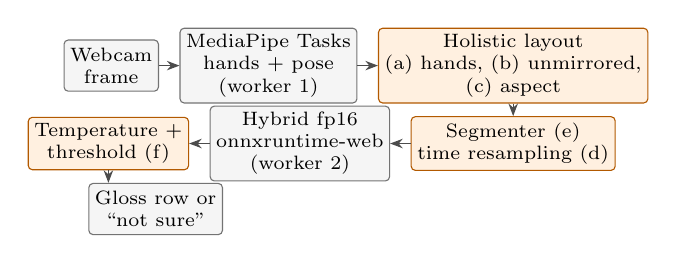
\begin{tikzpicture}[
  node distance=1.6mm and 2.6mm,
  box/.style={draw=black!55, rounded corners=1.5pt, fill=black!4, align=center, font=\scriptsize,
              inner sep=2.2pt, minimum height=6.5mm},
  live/.style={box, fill=orange!12, draw=orange!70!black},
  arr/.style={-{Stealth[length=1.6mm]}, black!70, line width=0.45pt}]
  \node[box] (cam) {Webcam\\frame};
  \node[box, right=of cam] (mp) {MediaPipe Tasks\\hands + pose\\(worker 1)};
  \node[live, right=of mp] (map) {Holistic layout\\(a) hands, (b) unmirrored,\\(c) aspect};
  \node[live, below=of map] (seg) {Segmenter (e)\\time resampling (d)};
  \node[box, left=of seg] (cls) {Hybrid fp16\\onnxruntime-web\\(worker 2)};
  \node[live, left=of cls] (dec) {Temperature +\\threshold (f)};
  \node[box, below=of dec, xshift=6mm] (out) {Gloss row or\\``not sure''};
  \draw[arr] (cam) -- (mp);
  \draw[arr] (mp) -- (map);
  \draw[arr] (map) -- (seg);
  \draw[arr] (seg) -- (cls);
  \draw[arr] (cls) -- (dec);
  \draw[arr] (dec.south) -- (dec.south |- out.north);
\end{tikzpicture}
\caption{The live pipeline in the browser. Orange boxes are the six audited steps; each reads its
constants from \cfg{features\_spec.json} or the model metadata, which the Python training code also
reads.}
\label{fig:pipeline}
\end{figure}

\subsection{Six candidate discrepancies}
\label{sec:faults}

\paragraph{(a) Hand slots.} Holistic, which produced the training data, crops each hand from the
pose, so its \emph{left hand} block is the hand at the signer's left wrist. The browser's
HandLandmarker reports a handedness label instead, and the shipped build mapped that label as if
the frame were mirrored while it ran detection on the unmirrored frame, so every hand went into the
wrong block. The fix assigns each detected hand to the block of the nearer pose wrist, Holistic's
own rule, and falls back to the label only when there is no pose.

\paragraph{(b) Mirroring.} The shipped build already detected landmarks on the unmirrored frame;
we test detection on the mirrored frame, as a selfie pipeline would do it, as a counterfactual.

\paragraph{(c) Aspect ratio.} Coordinates are normalized by the image width and height, so the
same body has different normalized proportions in a portrait phone recording and a wide webcam.
The shipped build corrected for this with a body-ratio estimate over the first two seconds. The fix
replaces it by a rule from the frame size: we estimate the training data's width-to-height ratio
from face geometry on the training split (\V{asp.train}) and rescale live y coordinates about the
shoulder midpoint by $k = r_{\mathrm{train}} / (w/h)$, with the real width and height of the frame.

\paragraph{(d) Frame rate.} Training resampled each sequence to \V{data.frames} frames by frame
index; the dataset has no timestamps. The browser's frame rate varies with the camera and the load,
so resampling by index stretches or compresses time; the fix resamples on the capture-time clock.

\paragraph{(e) Segmentation.} The shipped build segmented by hand presence: a segment starts after
\V{pres.start} frames with a hand and ends after \V{pres.end} without one or after \V{pres.max} s.
The fix is a state machine on motion energy, the speed of the wrist and fingertips in shoulder
widths per second on aspect-corrected coordinates, so (c) and (e) interact. A sign starts when a
hand is present and the energy exceeds \V{seg.start}, and ends when the hands are lost for
\V{seg.lostms} ms, stay below \V{seg.still} for \V{seg.stillms} ms, or after \V{seg.maxs} s;
segments shorter than \V{seg.minms} ms are discarded, and gaps up to \V{seg.gapms} ms are bridged.
The thresholds come from the validation sequences, assuming their frames are \V{seg.assumedfps} fps
apart: the start threshold is the \V{seg.startpct}th percentile of the per-sequence peak energy, and
the still threshold the largest value at which at most \V{seg.stillpct}\% of sequences would be cut
inside the sign.

\paragraph{(f) Calibration and abstention.} The shipped build showed the raw top-1 above a
threshold set for \V{cal.targetprec}\% precision on validation. The fix divides the logits by a
temperature fitted on validation (\V{cal.T}) and shows a word only if its probability reaches a
threshold chosen on validation to maximize the net score, coverage times twice the selective
accuracy minus one, so a correct accepted word gains one, a wrong one costs one and ``not sure''
scores zero \citep{guo2017calibration,geifman2017selective}.

\paragraph{One specification, one test.} The landmark subset, normalization, mirroring,
resampling, aspect constant and segmenter thresholds live in \cfg{features\_spec.json}, which
Python and the browser both read. A golden-fixture test runs the browser code on the raw landmarks
of \V{par.cases} validation sequences, exported from Python with Python's features and logits, and
requires every model input to match within \V{par.tol} and the top-1 class to agree; it covers hand
assignment and replays a stream through the segmenter frame by frame. It runs in continuous
integration, so a change to either implementation that alters a feature fails the build.

\subsection{Evaluation on new recordings}

\paragraph{Clips.} The author recorded \V{lg.clips} clips with a laptop webcam: \V{lg.signs}
signs from the vocabulary (\authortodo{how the signs were chosen, and the source of the sign
forms}), two takes each (median \V{lg.duration}\,s), unmirrored at \V{lg.width}$\times$\V{lg.height}
and about \V{lg.fps} frames per second (Figure~\ref{fig:skeleton} in the appendix), scaled to
\V{lg.ywidth}$\times$\V{lg.yheight} for both pipelines. No clip duplicates another. The author is
both the developer and the only signer, and the order of the fixes was motivated by a pilot of the
same person (Appendix~\ref{app:pilot}). Nothing was tuned on these clips: every threshold, the
temperature and the aspect constant come from the training and validation splits, and the analysis
was written into the configuration before the first run.

\paragraph{Pipelines.} \emph{Python + Holistic} runs legacy MediaPipe Holistic, the tracker that
produced the training data, on every frame and then the Python live pipeline; it is deterministic.
\emph{Browser + Tasks} runs the web app in Chrome on the target laptop with the clip as a fake
camera, in real time, so frames are dropped as they would be live. One browser per clip runs every
configuration in a seeded random order, so drift of the laptop does not fall on one configuration;
each configuration runs three times (Table~\ref{tab:livegapci} gives the count per row) and a clip's
score is its mean over the runs. In \V{lg.stalled} of \V{lg.browserrecords} browser records the
tracker processed fewer than half of the clip's frames; they are kept as measured. There are two
baselines: the \emph{shipped build} itself, which
runs MediaPipe and the classifier on the page's main thread at \V{lg.web.c0headbuild.fps}
frames per second, and \emph{as shipped}, the current app with the shipped build's settings at
\V{lg.web.c0asshipped.fps}.

\paragraph{Scoring and statistics.} A clip's prediction is the mean probability vector of its
classified segments; a clip without one counts as wrong. We report clip-level top-1 and top-3 with
percentile bootstrap intervals over clips \citep{efron1994bootstrap}. Each configuration is
compared with the one it modifies by a two-sided paired sign-flip permutation test on per-clip
scores \citep{dror2018hitchhiker}, and the p-values of each pipeline and metric are adjusted with
Holm's step-down procedure \citep{dror2017replicability}; the difference intervals are not adjusted.
This clip-level analysis was specified before the runs. Because the two takes of a sign are not
independent, we add a sensitivity analysis after the fact that treats each sign as one unit. The
families include comparisons that cannot change top-1 by construction, and error rates are
controlled within, not across, families. Power is low: to reach significance at the first Holm
step, at least \V{mde.web.k} clips (\V{mde.web.pts} points) must all move in one direction in the
browser and \V{mde.py.k} in Python, so smaller effects are inconclusive rather than absent
\citep{card2020power}.

\subsection{Results}
\label{sec:liveresults}

% Generated by scripts/paper_tables.py -- do not edit.
\typeout{[table livegap]}
\begin{table}[t]
\centering
\footnotesize
\setlength{\tabcolsep}{3pt}
\begin{tabular}{lrrrr}
\toprule
 & \multicolumn{2}{c}{Python} & \multicolumn{2}{c}{Browser} \\
\cmidrule(lr){2-3}\cmidrule(lr){4-5}
Config & top-1 & top-3 & top-1 & top-3 \\
\midrule
Shipped build & -- & -- & \V{lg.web.c0headbuild.top1} & \V{lg.web.c0headbuild.top3} \\
As shipped (v1 CNN) & \V{lg.py.c0asshipped.top1} & \V{lg.py.c0asshipped.top3} & \V{lg.web.c0asshipped.top1} & \V{lg.web.c0asshipped.top3} \\
+ v2 hybrid model & \V{lg.py.c1model.top1} & \V{lg.py.c1model.top3}$^{*}$ & \V{lg.web.c1model.top1}$^{*}$ & \V{lg.web.c1model.top3}$^{*}$ \\
+ hand assignment (a) & \V{lg.py.c2hands.top1}$^{*}$ & \V{lg.py.c2hands.top3}$^{*}$ & \V{lg.web.c2hands.top1}$^{*}$ & \V{lg.web.c2hands.top3}$^{*}$ \\
+ aspect from frame (c) & \V{lg.py.c3aspect.top1} & \V{lg.py.c3aspect.top3} & \V{lg.web.c3aspect.top1} & \V{lg.web.c3aspect.top3} \\
+ time resampling (d) & \V{lg.py.c4time.top1} & \V{lg.py.c4time.top3} & \V{lg.web.c4time.top1} & \V{lg.web.c4time.top3} \\
+ motion segmenter (e) & \V{lg.py.c5segmenter.top1} & \V{lg.py.c5segmenter.top3} & \V{lg.web.c5segmenter.top1} & \V{lg.web.c5segmenter.top3} \\
+ calibration (f): final & \V{lg.py.c6final.top1} & \V{lg.py.c6final.top3} & \V{lg.web.c6final.top1} & \V{lg.web.c6final.top3} \\
\midrule
final, old hand mapping & \V{lg.py.xhands.top1}$^{*}$ & \V{lg.py.xhands.top3}$^{*}$ & \V{lg.web.xhands.top1}$^{*}$ & \V{lg.web.xhands.top3}$^{*}$ \\
final, mirrored frame (b) & -- & -- & \V{lg.web.xmirrored.top1} & \V{lg.web.xmirrored.top3} \\
final, mirrored + old mapping & -- & -- & \V{lg.web.xmirroredlabel.top1} & \V{lg.web.xmirroredlabel.top3} \\
final, no aspect corr. & \V{lg.py.xaspectoff.top1} & \V{lg.py.xaspectoff.top3} & \V{lg.web.xaspectoff.top1} & \V{lg.web.xaspectoff.top3}$^{*}$ \\
final, body-ratio aspect & \V{lg.py.xaspectcalibrated.top1} & \V{lg.py.xaspectcalibrated.top3} & \V{lg.web.xaspectcalibrated.top1} & \V{lg.web.xaspectcalibrated.top3} \\
final, index resampling & \V{lg.py.xindex.top1} & \V{lg.py.xindex.top3} & \V{lg.web.xindex.top1} & \V{lg.web.xindex.top3} \\
final, presence segmenter & \V{lg.py.xpresence.top1} & \V{lg.py.xpresence.top3} & \V{lg.web.xpresence.top1} & \V{lg.web.xpresence.top3} \\
final, v1 CNN & \V{lg.py.xv1model.top1} & \V{lg.py.xv1model.top3} & \V{lg.web.xv1model.top1} & \V{lg.web.xv1model.top3} \\
\bottomrule
\end{tabular}
\caption{Live-gap ablation on the \V{lg.clips} webcam clips (\V{lg.signs} signs $\times$ 2 takes): clip-level top-1/top-3 (\%) for Python with MediaPipe Holistic and for the browser with MediaPipe Tasks. Upper block: one fix added per row; lower block: one fix of the final pipeline undone. Browser rows are means over three real-time runs. $^{*}$: the change against the row it modifies is significant after Holm correction within the pipeline and metric (clip as unit, as pre-specified). Top-1 intervals, raw and sign-level p-values are in Table~\ref{tab:livegapci}.}
\label{tab:livegap}
\end{table}


\begin{figure}[t]
\centering
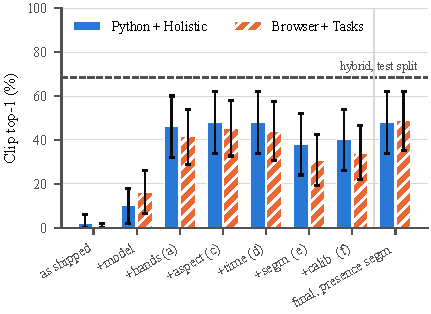
\includegraphics[width=\columnwidth]{figures/livegap}
\caption{Clip top-1 as the fixes are added one at a time, the final pipeline with presence
segmentation instead of the motion segmenter, and the hybrid's test top-1 (dashed); 95\%
bootstrap intervals over the \V{lg.clips} clips; browser bars are means over runs.}
\label{fig:livegap}
\end{figure}

Table~\ref{tab:livegap} and Figure~\ref{fig:livegap} give the ablation. The shipped build
recognized \V{lg.web.c0headbuild.top1}\% of the clips (top-3 \V{lg.web.c0headbuild.top3}\%). With
the hybrid and all fixes, clip top-1 reaches \V{lg.web.c6final.top1}\% \V{lg.web.c6final.top1ci}
in the browser and \V{lg.py.c6final.top1}\% \V{lg.py.c6final.top1ci} in Python (top-3
\V{lg.web.c6final.top3}\% and \V{lg.py.c6final.top3}\%). Measured from the hybrid with no fix,
this recovers \V{lg.web.recover}\% (browser) and \V{lg.py.recover}\% (Python) of the drop from its
\V{m.d.top1}\% test top-1, so most of the gap remains.

\paragraph{Hand slots had by far the largest effect.}
Adding the hand fix raised clip top-1 by \V{lg.py.c2hands.dtop1} points in Python and
\V{lg.web.c2hands.dtop1} in the browser (\V{lg.web.c2hands.dtop1better} clips better,
\V{lg.web.c2hands.dtop1worse} worse), and undoing it in the final pipeline cost
\V{lg.py.xhands.dtop1} and \V{lg.web.xhands.dtop1} points. In the pre-specified clip-level analysis
all four changes are significant after correction. With signs as the unit, they remain significant
in Python (Holm $p$ = \V{lg.py.c2hands.dtop1psign} and \V{lg.py.xhands.dtop1psign}) and for undoing
the fix in the browser (\V{lg.web.xhands.dtop1psign}), but not for adding it in the browser
(\V{lg.web.c2hands.dtop1psign}). Mirroring (b) was not a fault: detecting on the mirrored frame
changes little once hands are assigned by the pose (\V{lg.web.xmirrored.dtop1} points), and the
old label mapping fails with or without mirroring (\V{lg.web.xhands.top1}\% and
\V{lg.web.xmirroredlabel.top1}\%).

\paragraph{Aspect correction and segmentation: large but inconclusive.}
Removing all aspect correction from the final pipeline cost \V{lg.py.xaspectoff.dtop1} points in
Python and \V{lg.web.xaspectoff.dtop1} in the browser, and replacing presence segmentation by the
motion segmenter cost \V{lg.py.c5segmenter.dtop1} and \V{lg.web.c5segmenter.dtop1}; none of these
changes is significant after correction at either unit, so we treat them as inconclusive. The
shipped build's own aspect correction scored like the new rule (\V{lg.py.xaspectcalibrated.dtop1}
and \V{lg.web.xaspectcalibrated.dtop1} points), so the data show that some correction is needed,
not that the shipped one was wrong. The final pipeline with presence segmentation instead
(\cfg{x\_presence}) matches or beats every other configuration we measured,
\V{lg.py.xpresence.top1}\% in Python and \V{lg.web.xpresence.top1}\% in the browser. The motion segmenter's loss comes mostly from
whole signs it never segmented: \V{lg.py.c6final.noseg} clips in Python and
\V{lg.web.c6final.noseg} per browser run had no classified segment, against
\V{lg.py.xpresence.noseg} and \V{lg.web.xpresence.noseg} with presence segmentation, and the
segments it did cut were shorter (median \V{lg.web.c5segmenter.segms} against
\V{lg.web.c4time.segms} ms in the browser). Its thresholds assume the dataset's frames are
\V{seg.assumedfps} fps apart; if they are not, speeds are misestimated, which would produce missed
starts of this kind. We keep the pipeline as specified, because choosing a segmenter on these clips
would tune on the test.

\paragraph{The other changes.}
Swapping in the hybrid before any fix gained \V{lg.web.c1model.dtop1} points in the browser
(\V{lg.web.c1model.dtop1better} clips better, none worse; \V{lg.web.c1model.dtop1sig} at clip
level, not at sign level, Holm $p$ = \V{lg.web.c1model.dtop1psign}) and \V{lg.py.c1model.dtop1} in
Python, from a floor near zero. Resampling by time (d) cannot matter in Python, where the frame rate is constant and both clocks
give the same positions; in the browser it changed clip top-1 by \V{lg.web.c4time.dtop1} points.
Calibration (f) does not change a segment's top-1, though averaging over segments can move a clip's
(\V{lg.web.c6final.dtop1} points). Replacing the hybrid by the v1 CNN in the final pipeline cost
\V{lg.py.xv1model.dtop1} and \V{lg.web.xv1model.dtop1} points (\V{lg.web.xv1model.dtop1sig}), so
the hybrid's test-set advantage shows only weakly here.

\paragraph{What remains.}
The two pipelines differ by little: browser minus Python is \V{lg.pd.c6final.diff} points
\V{lg.pd.c6final.ci} for the final pipeline and \V{lg.pd.xpresence.diff} \V{lg.pd.xpresence.ci} with
presence segmentation (signs as the unit). The training tracker is therefore not what separates
these clips from the test split; the remaining gap lies in what both live pipelines share, above all
segmentation, or in the clips themselves (signer, camera, room and the signer's productions), which
this design cannot separate. \V{lg.failboth} of the \V{lg.signs} signs fail in every take in both
pipelines, and for \V{lg.sharedconf} the most frequent wrong guess is the same in both
(\V{lg.sharedconflist}; Table~\ref{tab:persign}).

\paragraph{Live abstention.}
On the live segments the calibration does not hold: the expected calibration error is
\V{lg.cal.web.ece} in the browser (\V{cal.test.ece1} on test). The validation threshold accepts
\V{lg.cal.web.cov}\% of segments at \V{lg.cal.web.sel}\% selective accuracy, a net score of
\V{lg.cal.web.net} against \V{cal.test.net} on test; it holds back \V{lg.cal.web.rejwrong}\% of
the wrong guesses but also \V{lg.cal.web.rejright}\% of the correct ones.

\section{System Demonstration}
\label{sec:system}

The recognizer ships as an installable web app that runs entirely in the browser. \emph{Translate},
despite its name, turns a sequence of isolated signs into a row of glosses; below the calibrated
threshold it shows ``not sure'' with the top three candidates and adds nothing until the user picks
one. \emph{Practice} shows a target sign and scores the next segment as correct (top-1), close
(top-3) or wrong. \emph{Signs} lists the vocabulary with a link to a dictionary video per sign. On
request, a serverless proxy sends only the recognized glosses to a hosted language model
(\cfg{llama-3.1-8b-instant} on Groq) with a fixed instruction to write one short sentence without
adding facts, and the browser speaks it; offline, a rule-based joiner produces a sentence marked as
basic. \textbf{Sentence generation is not evaluated}; a fluent sentence can lend false authority to
wrong glosses and omits the grammar ASL carries in space, movement and the face. Video never leaves
the device, and a service worker caches the model for offline use and adds the cross-origin
isolation headers that WebAssembly threads need on static hosting.

\section{Conclusion}
\label{sec:conclusion}

A signer-independent test accuracy of \V{m.d.top1}\% did not make a usable live recognizer: the
first deployment recognized \V{lg.web.c0headbuild.top1}\% of new webcam clips. Of six candidate
train--serve discrepancies, one had a large and consistent effect: putting each hand in a different
slot from the one the training tracker used. A shared feature specification and a golden parity
test, which covers hand assignment, now keep the Python and browser pipelines identical and fail
when they diverge. With the fixes, clip top-1 reaches \V{lg.web.c6final.top1}\% in the browser and
\V{lg.py.c6final.top1}\% with the training tracker, about \V{lg.web.recover}--\V{lg.py.recover}\%
of the way back to test accuracy. The rest of the gap is shared by both live pipelines. Part of it
is a segmenter, tuned on dataset sequences, that missed whole signs; the rest may be the signer,
the camera or the signer's productions, which one signer cannot separate. Thresholds chosen on
dataset sequences need live validation data of their own, and the next steps are an oracle
segmentation of these clips and live recordings from many Deaf signers, gathered with their
involvement.

% ACL convention: Limitations and the ethics statement follow the conclusion and do not count
% toward the page limit.
\section*{Limitations}

\paragraph{One signer in the live test.} The live evaluation uses \V{lg.clips} clips recorded by a
single signer, the author (\authortodo{state your ASL experience}), in one room with one laptop
camera. If the signer's productions differ from the dataset's signers, some live errors are
production differences rather than pipeline or camera effects, and nothing in this design
separates them; a rating of each clip by a fluent, ideally Deaf, signer would. The results show
which pipeline discrepancies matter for this signer and camera; they do not estimate accuracy for
Deaf signers in general. With fifty clips most effects below the detection limit stated in
Section~\ref{sec:livegap} are inconclusive. The ten-clip pilot was recorded by the same person.

\paragraph{Controls we did not run.} Two controls would locate the remaining gap: running the live
pipeline on test-split landmark sequences, which measures what the live code costs in
distribution, and an oracle segmentation of the live clips, which separates segmentation from
recognition. The segmenter's thresholds rest on an assumed dataset frame rate. We also did not
disentangle architecture from model size or recipe in the v2 ablation.

\paragraph{Isolated signs from a closed vocabulary.} The model recognizes \V{data.signs} isolated
signs. It does not handle continuous signing, fingerspelling, or signs outside the vocabulary,
which it maps to the nearest known sign unless the confidence threshold rejects them. It is not a
translator: the gloss row and the generated sentence drop the grammar that ASL carries in space,
movement and facial expression.

\paragraph{Language and population.} The data is American Sign Language. The author is based in
India, where Indian Sign Language is the relevant language; nothing here transfers to it without
new data, such as INCLUDE \citep{sridhar2020include}. We know only the number of signers in the
dataset (\V{data.signers}), not their demographics, hearing status or fluency, so we cannot say
for whom the model works less well.

\paragraph{Test-set statistics and reuse.} With \V{data.testsigners} test signers, sequence-level
tests treat thousands of sequences from the same person as independent; the per-signer results
(Table~\ref{tab:persigner}) are the more conservative evidence, and a four-of-four split can never
be significant on its own. The test split was evaluated several times during development
(Table~\ref{tab:testaccess}), so its numbers are less clean than a single final evaluation.

\paragraph{Hardware and trackers.} Browser timings come from one laptop and one browser version;
the CPU fallback of MediaPipe reaches only \V{t.cpu.fps} frames per second there
(Section~\ref{sec:efficiency}).

\section*{Ethics Statement}

\paragraph{No evaluation with Deaf users.} We did not evaluate the system with Deaf or
hard-of-hearing users, and no Deaf signer took part in its design. Sign language technology
should be built with, and ideally led by, Deaf communities \citep{bragg2019interdisciplinary,
yin2021including,fox2023bestpractices}, and Deaf researchers have criticized how often the field
sets its agenda without them \citep{desai2024systemic}. This paper is an engineering study of one
failure mode, the train--serve gap, and not a claim of usefulness to the people the technology is
meant for.

\paragraph{Practice mode can mislead learners.} Deaf children of hearing parents are at risk of
language deprivation when no one around them signs \citep{humphries2012deprivation}, and practice
tools are one motivation for this work. At the live accuracy we measured, however, the Practice
mode would tell a learner that many correctly produced signs are wrong, and for some signs it fails
every time; it could discourage learners or teach them to distort signs to please the model. It
should report low-confidence results as ``not sure'' rather than ``try again'', state per-sign
reliability, and be evaluated with learners and Deaf teachers before anyone relies on it.

\paragraph{Overstating translation.} Calling a gloss classifier a translator misleads users about
what it understands, and the app's main mode is still named \emph{Translate}. The app states that it
recognizes a fixed set of isolated signs and is not a full ASL translator, shows ``not sure'' below
its threshold, and labels rule-based sentences as basic, but a fluent generated sentence can lend
false authority to wrong glosses. A tool that misrecognizes signs could cause harm if relied on in
important conversations; it must not replace interpreters, and a name such as ``Recognize'' would
describe the mode better.

\paragraph{Data and consent.} The training data is the public Google ISLR release (CC BY 4.0) of
landmarks, not video. The live clips show the author of this paper, who recorded them and consents
to their use here; they are not released, and every figure in the paper shows landmarks only,
never camera pixels. The app processes video on the device; when the user asks for a sentence, the
recognized glosses, and nothing else, are sent to a third-party language model provider.


\section*{Acknowledgments}
\textbf{AI assistance disclosure:} TODO-AUTHOR-WRITES-THIS

\bibliography{references}

\appendix
\section{Hyperparameters, Features and Model Selection}
\label{app:hparams}

% Generated by scripts/paper_tables.py -- do not edit.
\typeout{[table hparams]}
\begin{table*}[t]
\centering
\footnotesize
\begin{tabular}{lp{12.5cm}}
\toprule
Setting & Value (from the run configs) \\
\midrule
GRU (v1) & proj dim 192, hidden size 128, num layers 2, input dropout 0.2, rnn dropout 0.2, head dropout 0.3 \\
CNN (v1) & channels 192, num blocks 6, kernel size 5, block dropout 0.2, head dropout 0.3 \\
Transformer (v1) & d model 192, num layers 4, num heads 4, ff dim 384, dropout 0.1, head dropout 0.3 \\
Hybrid (v2) & dim 256, num stages 3, conv blocks 2, kernel size 17, expansion dim 512, conv dropout 0.2, num heads 4, ff dim 512, attention dropout 0.1, head dropout 0.4, late dropout start 0.5 \\
v1 recipe & epochs 60, batch size 256, lr 0.001, weight decay 0.05, warmup fraction 0.05, label smoothing 0.1, grad clip 1.0, patience 15; augmentation: affine p 0.8, temporal p 0.5, jitter p 0.5 \\
v2 recipe & epochs 150, batch size 256, lr 0.0005, weight decay 0.05, warmup fraction 0.05, label smoothing 0.1, grad clip 1.0, patience 30, EMA decay 0.999; augmentation: affine p 0.8, temporal p 0.5, jitter p 0.5, rotation deg 15.0, scale min 0.85, scale max 1.15, translate 0.1, window min 0.8, jitter std 0.01, frame dropout p 0.5, time mask p 0.5, landmark mask p 0.3, hand rotation p 0.5 \\
\bottomrule
\end{tabular}
\caption{Hyperparameters, read from \cfg{experiments/train\_*.yaml} (v1) and the hybrid run's \cfg{config.yaml} (v2). Every signer-independent configuration was trained with seeds 0, 1 and 2.}
\label{tab:hparams}
\end{table*}


\paragraph{Dominant-hand mirroring.}
\label{app:mirror}
Mirroring flips \V{data.mirroredpct}\% of the Google ISLR sequences, but it is a property of
signers rather than sequences: \V{mir.high} of the \V{data.signers} signers have
more than 80\% of their sequences mirrored and \V{mir.low} have under 5\%, consistent with left-handed signers or
mirrored (selfie) recordings, which the data cannot tell apart. Every test signer is at most
\V{mir.testmax}\%.

\paragraph{Model selection.} Figure~\ref{fig:acclat} shows the candidates against the shipping
rule's latency budget (Section~\ref{sec:models}).

\begin{figure}[t]
\centering
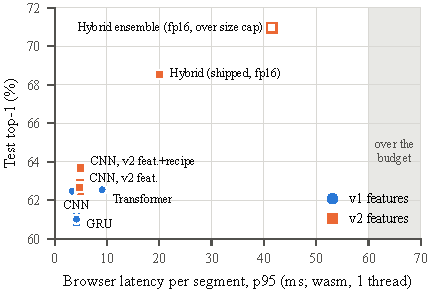
\includegraphics[width=\columnwidth]{figures/acc_latency}
\caption{Test top-1 (mean $\pm$ sd over seeds) against browser latency per call (p95, Chrome on
the i3-1115G4, wasm, one thread; selection benchmark). The hybrid ensemble is within the latency
budget but over the size cap; the single hybrid (fp16) is the most accurate model that meets both.}
\label{fig:acclat}
\end{figure}

\section{Test Signers and Test-Split Access}
\label{app:testsplit}

Table~\ref{tab:persigner} gives every signer-independent model's top-1 per Google ISLR test
signer; Table~\ref{tab:testaccess} lists every logged access to either test split, including v3's
single access to each.

% Generated by scripts/paper_tables.py -- do not edit.
\typeout{[table persigner]}
\begin{table}[t]
\centering
\footnotesize
\setlength{\tabcolsep}{3pt}
\begin{tabular}{lrrrr}
\toprule
Model & S1 & S2 & S3 & S4 \\
\midrule
CNN (v1) & 46.0 & 71.5 & 57.4 & 69.2 \\
Transformer (v1) & 46.7 & 71.4 & 55.6 & 71.1 \\
GRU (v1) & 44.7 & 70.4 & 54.7 & 68.6 \\
CNN, v2 features & 45.3 & 71.0 & 57.3 & 70.9 \\
CNN, v2 features + recipe & 45.5 & 72.2 & 58.9 & 71.6 \\
Hybrid & 51.9 & 77.7 & 61.2 & 77.6 \\
\bottomrule
\end{tabular}
\caption{Test top-1 (\%, mean over seeds) for each of the four test signers (S1--S4: 2700, 4322, 4787, 4433 sequences).}
\label{tab:persigner}
\end{table}

% Generated by scripts/paper_tables.py -- do not edit.
\typeout{[table testaccess]}
\begin{table}[t]
\centering
\footnotesize
\setlength{\tabcolsep}{3pt}
\begin{tabular}{llp{4.0cm}}
\toprule
Date (UTC) & Commit & Evaluated on test \\
\midrule
2026-11-04 & 43806b4+ & signer-dependent v1, v1 models \\
2026-11-04 & d34f874+ & quantized v1 variants \\
2026-11-06 & 3fbafa3+ & v2 models \\
2026-11-15 & 3fbafa3+ & signer-dependent v1, v1 models, v2 models \\
2026-11-16 & 36219ea+ & v1 models, v2 models, shipped ONNX file (saved logits for this paper) \\
2026-11-17 & 36219ea+ & shipped ONNX file (saved logits for this paper) \\
\bottomrule
\end{tabular}
\caption{Every logged run of the only script that reads the test split (\cfg{results/final*/test\_access\_log.json}); + marks a working tree with uncommitted changes. The v2 models were designed after the v1 evaluation in the first row.}
\label{tab:testaccess}
\end{table}


\section{ASL Citizen, v3 and Teach Dex}
\label{app:v3}

\paragraph{ASL Citizen.} Table~\ref{tab:citizen} breaks the ASL Citizen test results down by how
each label was mapped. v2 is weakest on signs mapped through a numbered variant; v3, trained on
the same mapping, is about equally accurate under all three rules, which says nothing about
whether the mapping is right. With each model's own validation temperature, v2's expected
calibration error on this split is \V{cit.v2.ece} and v3's \V{cit.v3.ece}.

\paragraph{v3 training.} v3 uses the v2 hybrid's architecture and recipe
(Table~\ref{tab:hparams}) with \V{v3.train} training and \V{v3.val} validation sequences from
\V{v3.trainsigners} and \V{v3.valsigners} signers (\V{v3.valsigners.ks} Google ISLR and
\V{v3.valsigners.cit} ASL Citizen validation signers; one of ASL Citizen's \V{cit.all.valsigners}
has no kept video of a mapped sign); its Google ISLR test split is the same as v2's.
The \V{v3.seeds} seeds scored between \V{v3.selmin}\% and \V{v3.selmax}\% on the selection
criterion, the mean of the two validation top-1 scores; a seed took about \V{v3.trainmin}
minutes on a \V{v3.gpu}.

\paragraph{Teach Dex.} The blend's weight and offset minimize the mean negative log-likelihood
over \V{td.draws} simulated draws on validation signers: in each, one signer teaches between one
and twenty-five signs with \V{td.examples} of their own sequences each, and every other sequence
of that signer is a query, taught sign or not. ASL Citizen's validation signers recorded most signs
once or twice, too few for this simulation, so v3's blend is fitted on the Google ISLR part of its
validation split, with the same draws as v2's. The blends (weight \V{td.v2.weight}, offset
\V{td.v2.offset} for v2; \V{td.v3.weight} and \V{td.v3.offset} for v3) raise validation top-1 on
taught signs from \V{td.v2.valbefore}\% to \V{td.v2.valafter}\% (v2) and from \V{td.v3.valbefore}\%
to \V{td.v3.valafter}\% (v3), and leave untaught signs where they were (\V{td.v2.valuntaught0}\%
and \V{td.v2.valuntaught1}\%; \V{td.v3.valuntaught0}\% and \V{td.v3.valuntaught1}\%).

\paragraph{The compromised v3 run of Teach Dex.} Its model-alone score on take 2,
\V{td.v3.model}\%, is far below v3's \V{lg3.web.v3.take2}\% on the same clips in the live runs of
Section~\ref{sec:liveresults} (for v2 the two agree, \V{td.v2.model}\% and \V{lg3.web.v2.take2}\%),
and its runs found ever fewer segments (\V{td.v3.segmax} down to \V{td.v3.segmin}, against
\V{td.v2.segmin}--\V{td.v2.segmax} with v2), for a reason the harness, which logs no frame rate,
cannot show. Clips without a segment cannot change, so v3's gain (\V{td.v3.diff} points, $p$ =
\V{td.v3.p}) is biased toward zero and says nothing about teaching v3.

% Generated by scripts/paper_tables.py -- do not edit.
\typeout{[table citizen]}
\begin{table}[t]
\centering
\footnotesize
\setlength{\tabcolsep}{3pt}
\begin{tabular}{lrrr}
\toprule
ASL Citizen test & Videos & v2 & v3 \\
\midrule
Top-1, exact name & \V{cit.rule.exact} & \V{cit.v2.exact} & \V{cit.v3.exact} \\
Top-1, numbered variant & \V{cit.rule.variant} & \V{cit.v2.variant} & \V{cit.v3.variant} \\
Top-1, synonym & \V{cit.rule.synonym} & \V{cit.v2.synonym} & \V{cit.v3.synonym} \\
Top-1, all & \V{cit.videos} & \V{cit.v2.top1} & \V{cit.v3.top1} \\
Top-3, all & & \V{cit.v2.top3} & \V{cit.v3.top3} \\
Top-1, range over signers & & \V{cit.v2.sigmin}--\V{cit.v2.sigmax} & \V{cit.v3.sigmin}--\V{cit.v3.sigmax} \\
\midrule
ECE, raw softmax & & \V{cit.v2.eceraw} & \V{cit.v3.eceraw} \\
ECE, temperature from val & & \V{cit.v2.ece} & \V{cit.v3.ece} \\
Coverage at val threshold & & \V{cit.v2.cov} & \V{cit.v3.cov} \\
Selective accuracy & & \V{cit.v2.sel} & \V{cit.v3.sel} \\
\bottomrule
\end{tabular}
\caption{v2 and v3 on the official ASL Citizen test split (\%, except ECE), by how the sign's label was mapped to an ASL Citizen gloss. Each model was evaluated once (\cfg{scripts/citizen\_eval.py}); the mapping is AI-assisted and unconfirmed by a signer. v3 trained on ASL Citizen's training signers.}
\label{tab:citizen}
\end{table}


\section{Calibration}
\label{app:calib}

Figure~\ref{fig:calibration} shows the deployed v2 model before and after temperature scaling.
Before scaling the model is underconfident, as a temperature below one implies
(Section~\ref{sec:models}).

\begin{figure}[t]
\centering
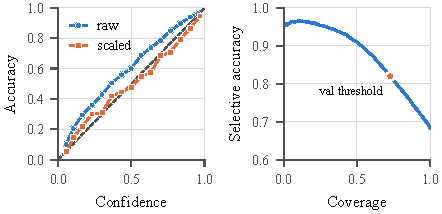
\includegraphics[width=\columnwidth]{figures/calibration}
\caption{The deployed v2 model on the Google ISLR test split. Left: reliability diagram before (raw)
and after temperature scaling (bins with at least fifty sequences); after scaling the upper bins
are slightly overconfident. Right: selective accuracy against coverage when accepting the most
confident predictions first; the dot is the threshold chosen on validation.}
\label{fig:calibration}
\end{figure}

\section{Quantization}
\label{app:quant}

Table~\ref{tab:quant} and Figure~\ref{fig:quant} give every post-training quantization variant of
the v1 models (Section~\ref{sec:efficiency}).

% Generated by scripts/paper_tables.py -- do not edit.
\typeout{[table quant]}
\begin{table}[t]
\centering
\footnotesize
\setlength{\tabcolsep}{3pt}
\begin{tabular}{llrrrr}
\toprule
Model & Variant & Top-1 & $\Delta$ & MB & p50 (ms) \\
\midrule
CNN & fp32 & 62.5 & +0.0 & 1.29 & 0.56 \\
 & fp16 & 62.5 & +0.0 & 0.67 & 0.69 \\
 & int8 dyn. & 59.3 & $-$3.1 & 0.39 & 4.78 \\
 & int8 st. & 55.7 & $-$6.8 & 0.46 & 0.64 \\
 & int8 full & 56.1 & $-$6.4 & 0.46 & 0.64 \\
\midrule
GRU & fp32 & 61.0 & +0.0 & 2.86 & 1.08 \\
 & fp16 & 61.0 & $-$0.0 & 1.44 & 1.07 \\
 & int8 dyn. & 58.4 & $-$2.7 & 2.37 & 0.99 \\
 & int8 st. & 50.6 & $-$10.4 & 2.38 & 1.02 \\
 & int8 full & 51.3 & $-$9.7 & 2.38 & 1.07 \\
\midrule
Transf. & fp32 & 62.5 & +0.0 & 5.19 & 1.56 \\
 & fp16 & 62.5 & $-$0.0 & 2.65 & 1.97 \\
 & int8 dyn. & 59.7 & $-$2.9 & 1.48 & 0.93 \\
 & int8 st. & 57.9 & $-$4.7 & 1.52 & 1.16 \\
 & int8 full & 58.6 & $-$4.0 & 1.52 & 1.39 \\
\midrule
Hybrid & fp32 & -- & -- & 13.70 & 4.10 \\
 & fp16 & -- & -- & 6.93 & 4.42 \\
 & int8 dyn. & -- & -- & 3.66 & 21.96 \\
\bottomrule
\end{tabular}
\caption{Post-training quantization of the v1 models (test top-1 \%, mean over seeds; $\Delta$ against fp32 in points) and CPU latency of one call in Python onnxruntime on the i3-1115G4 (1 intra-op thread, median p50 over three rounds, seed 0). dyn.: dynamic; st.: static with the feature block kept in float; full: static with the input and feature block quantized too. The hybrid has no int8 test evaluation (only latency and size).}
\label{tab:quant}
\end{table}


\begin{figure*}[t]
\centering
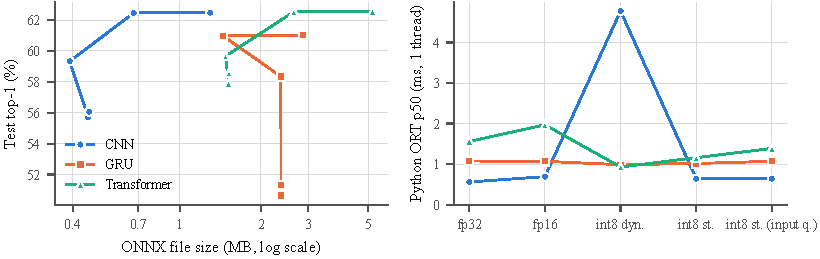
\includegraphics[width=0.9\textwidth]{figures/quant}
\caption{Post-training quantization of the v1 models. Left: test top-1 against file size (each
line runs through fp32, fp16, dynamic int8, static int8 and static int8 with the input quantized).
Right: one call in Python onnxruntime on the i3-1115G4 (1 thread, p50). Numbers are in
Table~\ref{tab:quant}.}
\label{fig:quant}
\end{figure*}

\section{Live-Gap Details}
\label{app:livegap}

\begin{figure}[t]
\centering
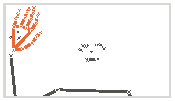
\includegraphics[width=0.6\columnwidth]{figures/skeleton}
\caption{One frame of a live clip (``hello''), drawn from its Holistic landmarks only: pose in
grey, the signer's right hand in orange. No camera image appears in this paper.}
\label{fig:skeleton}
\end{figure}

\paragraph{Segmenter.} A sign starts when a hand is present and the motion energy exceeds
\V{seg.start}, and ends when the hands are lost for \V{seg.lostms} ms, stay below \V{seg.still} for
\V{seg.stillms} ms, or after \V{seg.maxs} s; segments shorter than \V{seg.minms} ms are discarded and
gaps up to \V{seg.gapms} ms are bridged. The thresholds come from the validation sequences,
assuming their frames are \V{seg.assumedfps} fps apart: the start threshold is the
\V{seg.startpct}th percentile of the per-sequence peak energy, and the still threshold the largest
value at which at most \V{seg.stillpct}\% of sequences would be cut inside the sign.

\paragraph{Other changes.} Swapping in the hybrid before any fix gained \V{lg.web.c1model.dtop1}
points in the browser (\V{lg.web.c1model.dtop1better} clips better, none worse;
\V{lg.web.c1model.dtop1sig} at clip level, not at sign level, Holm $p$ =
\V{lg.web.c1model.dtop1psign}) and \V{lg.py.c1model.dtop1} in Python, from a floor near zero.
Resampling by time (d), which cannot matter in Python, changed browser clip top-1 by
\V{lg.web.c4time.dtop1} points, and calibration (f), which cannot change a segment's top-1, by
\V{lg.web.c6final.dtop1}. Replacing the hybrid by the v1 CNN in the final pipeline cost
\V{lg.py.xv1model.dtop1} and \V{lg.web.xv1model.dtop1} points (\V{lg.web.xv1model.dtop1sig}), so
the hybrid's test-set advantage shows only weakly here.

Figure~\ref{fig:skeleton} shows one frame of a live clip as the pipelines see it, and
Figure~\ref{fig:livegap} plots the ablation of Table~\ref{tab:livegap}.
Table~\ref{tab:livegapci} gives every live-gap configuration with its interval and its comparison
against the configuration it changes; Table~\ref{tab:persign} gives the final pipeline per sign,
next to the deployed v2 model's accuracy on the same sign in the test split. The most frequent
confusions of the final pipeline were, for Python + Holistic: \V{lg.py.confusions}; and for the
browser: \V{lg.web.confusions} (counts over takes and runs).

\begin{figure}[t]
\centering
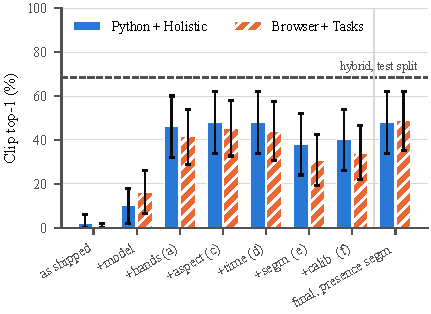
\includegraphics[width=\columnwidth]{figures/livegap}
\caption{Clip top-1 as the fixes are added one at a time, the final pipeline with presence
segmentation instead of the motion segmenter, and the hybrid's test top-1 (dashed); 95\%
bootstrap intervals over the \V{lg.clips} clips; browser bars are means over runs.}
\label{fig:livegap}
\end{figure}

% Generated by scripts/paper_tables.py -- do not edit.
\typeout{[table livegap_ci]}
\begin{table*}[t]
\centering
\footnotesize
\setlength{\tabcolsep}{2pt}
\begin{tabular}{llrrrrrrl}
\toprule
Pipeline & Config & Runs & top-1 [95\% CI] & $\Delta$ top-1 [95\% CI] & $p$ & $p_{\mathrm{Holm}}$ & $p_{\mathrm{Holm}}$, sign & Better/worse \\
\midrule
Python & As shipped (v1 CNN) & \V{lg.py.c0asshipped.runs} & \V{lg.py.c0asshipped.top1} \V{lg.py.c0asshipped.top1ci} & -- & -- & -- & -- & -- \\
Python & + v2 hybrid model & \V{lg.py.c1model.runs} & \V{lg.py.c1model.top1} \V{lg.py.c1model.top1ci} & \V{lg.py.c1model.dtop1} \V{lg.py.c1model.dtop1ci} & \V{lg.py.c1model.dtop1praw} & \V{lg.py.c1model.dtop1p} & \V{lg.py.c1model.dtop1psign} & \V{lg.py.c1model.dtop1better}/\V{lg.py.c1model.dtop1worse} \\
Python & + hand assignment (a) & \V{lg.py.c2hands.runs} & \V{lg.py.c2hands.top1} \V{lg.py.c2hands.top1ci} & \V{lg.py.c2hands.dtop1} \V{lg.py.c2hands.dtop1ci} & \V{lg.py.c2hands.dtop1praw} & \V{lg.py.c2hands.dtop1p} & \V{lg.py.c2hands.dtop1psign} & \V{lg.py.c2hands.dtop1better}/\V{lg.py.c2hands.dtop1worse} \\
Python & + aspect from frame (c) & \V{lg.py.c3aspect.runs} & \V{lg.py.c3aspect.top1} \V{lg.py.c3aspect.top1ci} & \V{lg.py.c3aspect.dtop1} \V{lg.py.c3aspect.dtop1ci} & \V{lg.py.c3aspect.dtop1praw} & \V{lg.py.c3aspect.dtop1p} & \V{lg.py.c3aspect.dtop1psign} & \V{lg.py.c3aspect.dtop1better}/\V{lg.py.c3aspect.dtop1worse} \\
Python & + time resampling (d) & \V{lg.py.c4time.runs} & \V{lg.py.c4time.top1} \V{lg.py.c4time.top1ci} & \V{lg.py.c4time.dtop1} \V{lg.py.c4time.dtop1ci} & \V{lg.py.c4time.dtop1praw} & \V{lg.py.c4time.dtop1p} & \V{lg.py.c4time.dtop1psign} & \V{lg.py.c4time.dtop1better}/\V{lg.py.c4time.dtop1worse} \\
Python & + motion segmenter (e) & \V{lg.py.c5segmenter.runs} & \V{lg.py.c5segmenter.top1} \V{lg.py.c5segmenter.top1ci} & \V{lg.py.c5segmenter.dtop1} \V{lg.py.c5segmenter.dtop1ci} & \V{lg.py.c5segmenter.dtop1praw} & \V{lg.py.c5segmenter.dtop1p} & \V{lg.py.c5segmenter.dtop1psign} & \V{lg.py.c5segmenter.dtop1better}/\V{lg.py.c5segmenter.dtop1worse} \\
Python & + calibration (f): final & \V{lg.py.c6final.runs} & \V{lg.py.c6final.top1} \V{lg.py.c6final.top1ci} & \V{lg.py.c6final.dtop1} \V{lg.py.c6final.dtop1ci} & \V{lg.py.c6final.dtop1praw} & \V{lg.py.c6final.dtop1p} & \V{lg.py.c6final.dtop1psign} & \V{lg.py.c6final.dtop1better}/\V{lg.py.c6final.dtop1worse} \\
Python & final, old hand mapping & \V{lg.py.xhands.runs} & \V{lg.py.xhands.top1} \V{lg.py.xhands.top1ci} & \V{lg.py.xhands.dtop1} \V{lg.py.xhands.dtop1ci} & \V{lg.py.xhands.dtop1praw} & \V{lg.py.xhands.dtop1p} & \V{lg.py.xhands.dtop1psign} & \V{lg.py.xhands.dtop1better}/\V{lg.py.xhands.dtop1worse} \\
Python & final, no aspect corr. & \V{lg.py.xaspectoff.runs} & \V{lg.py.xaspectoff.top1} \V{lg.py.xaspectoff.top1ci} & \V{lg.py.xaspectoff.dtop1} \V{lg.py.xaspectoff.dtop1ci} & \V{lg.py.xaspectoff.dtop1praw} & \V{lg.py.xaspectoff.dtop1p} & \V{lg.py.xaspectoff.dtop1psign} & \V{lg.py.xaspectoff.dtop1better}/\V{lg.py.xaspectoff.dtop1worse} \\
Python & final, body-ratio aspect & \V{lg.py.xaspectcalibrated.runs} & \V{lg.py.xaspectcalibrated.top1} \V{lg.py.xaspectcalibrated.top1ci} & \V{lg.py.xaspectcalibrated.dtop1} \V{lg.py.xaspectcalibrated.dtop1ci} & \V{lg.py.xaspectcalibrated.dtop1praw} & \V{lg.py.xaspectcalibrated.dtop1p} & \V{lg.py.xaspectcalibrated.dtop1psign} & \V{lg.py.xaspectcalibrated.dtop1better}/\V{lg.py.xaspectcalibrated.dtop1worse} \\
Python & final, index resampling & \V{lg.py.xindex.runs} & \V{lg.py.xindex.top1} \V{lg.py.xindex.top1ci} & \V{lg.py.xindex.dtop1} \V{lg.py.xindex.dtop1ci} & \V{lg.py.xindex.dtop1praw} & \V{lg.py.xindex.dtop1p} & \V{lg.py.xindex.dtop1psign} & \V{lg.py.xindex.dtop1better}/\V{lg.py.xindex.dtop1worse} \\
Python & final, presence segmenter & \V{lg.py.xpresence.runs} & \V{lg.py.xpresence.top1} \V{lg.py.xpresence.top1ci} & \V{lg.py.xpresence.dtop1} \V{lg.py.xpresence.dtop1ci} & \V{lg.py.xpresence.dtop1praw} & \V{lg.py.xpresence.dtop1p} & \V{lg.py.xpresence.dtop1psign} & \V{lg.py.xpresence.dtop1better}/\V{lg.py.xpresence.dtop1worse} \\
Python & final, v1 CNN & \V{lg.py.xv1model.runs} & \V{lg.py.xv1model.top1} \V{lg.py.xv1model.top1ci} & \V{lg.py.xv1model.dtop1} \V{lg.py.xv1model.dtop1ci} & \V{lg.py.xv1model.dtop1praw} & \V{lg.py.xv1model.dtop1p} & \V{lg.py.xv1model.dtop1psign} & \V{lg.py.xv1model.dtop1better}/\V{lg.py.xv1model.dtop1worse} \\
\midrule
Browser & Shipped build & \V{lg.web.c0headbuild.runs} & \V{lg.web.c0headbuild.top1} \V{lg.web.c0headbuild.top1ci} & -- & -- & -- & -- & -- \\
Browser & As shipped (v1 CNN) & \V{lg.web.c0asshipped.runs} & \V{lg.web.c0asshipped.top1} \V{lg.web.c0asshipped.top1ci} & -- & -- & -- & -- & -- \\
Browser & + v2 hybrid model & \V{lg.web.c1model.runs} & \V{lg.web.c1model.top1} \V{lg.web.c1model.top1ci} & \V{lg.web.c1model.dtop1} \V{lg.web.c1model.dtop1ci} & \V{lg.web.c1model.dtop1praw} & \V{lg.web.c1model.dtop1p} & \V{lg.web.c1model.dtop1psign} & \V{lg.web.c1model.dtop1better}/\V{lg.web.c1model.dtop1worse} \\
Browser & + hand assignment (a) & \V{lg.web.c2hands.runs} & \V{lg.web.c2hands.top1} \V{lg.web.c2hands.top1ci} & \V{lg.web.c2hands.dtop1} \V{lg.web.c2hands.dtop1ci} & \V{lg.web.c2hands.dtop1praw} & \V{lg.web.c2hands.dtop1p} & \V{lg.web.c2hands.dtop1psign} & \V{lg.web.c2hands.dtop1better}/\V{lg.web.c2hands.dtop1worse} \\
Browser & + aspect from frame (c) & \V{lg.web.c3aspect.runs} & \V{lg.web.c3aspect.top1} \V{lg.web.c3aspect.top1ci} & \V{lg.web.c3aspect.dtop1} \V{lg.web.c3aspect.dtop1ci} & \V{lg.web.c3aspect.dtop1praw} & \V{lg.web.c3aspect.dtop1p} & \V{lg.web.c3aspect.dtop1psign} & \V{lg.web.c3aspect.dtop1better}/\V{lg.web.c3aspect.dtop1worse} \\
Browser & + time resampling (d) & \V{lg.web.c4time.runs} & \V{lg.web.c4time.top1} \V{lg.web.c4time.top1ci} & \V{lg.web.c4time.dtop1} \V{lg.web.c4time.dtop1ci} & \V{lg.web.c4time.dtop1praw} & \V{lg.web.c4time.dtop1p} & \V{lg.web.c4time.dtop1psign} & \V{lg.web.c4time.dtop1better}/\V{lg.web.c4time.dtop1worse} \\
Browser & + motion segmenter (e) & \V{lg.web.c5segmenter.runs} & \V{lg.web.c5segmenter.top1} \V{lg.web.c5segmenter.top1ci} & \V{lg.web.c5segmenter.dtop1} \V{lg.web.c5segmenter.dtop1ci} & \V{lg.web.c5segmenter.dtop1praw} & \V{lg.web.c5segmenter.dtop1p} & \V{lg.web.c5segmenter.dtop1psign} & \V{lg.web.c5segmenter.dtop1better}/\V{lg.web.c5segmenter.dtop1worse} \\
Browser & + calibration (f): final & \V{lg.web.c6final.runs} & \V{lg.web.c6final.top1} \V{lg.web.c6final.top1ci} & \V{lg.web.c6final.dtop1} \V{lg.web.c6final.dtop1ci} & \V{lg.web.c6final.dtop1praw} & \V{lg.web.c6final.dtop1p} & \V{lg.web.c6final.dtop1psign} & \V{lg.web.c6final.dtop1better}/\V{lg.web.c6final.dtop1worse} \\
Browser & final, old hand mapping & \V{lg.web.xhands.runs} & \V{lg.web.xhands.top1} \V{lg.web.xhands.top1ci} & \V{lg.web.xhands.dtop1} \V{lg.web.xhands.dtop1ci} & \V{lg.web.xhands.dtop1praw} & \V{lg.web.xhands.dtop1p} & \V{lg.web.xhands.dtop1psign} & \V{lg.web.xhands.dtop1better}/\V{lg.web.xhands.dtop1worse} \\
Browser & final, mirrored frame (b) & \V{lg.web.xmirrored.runs} & \V{lg.web.xmirrored.top1} \V{lg.web.xmirrored.top1ci} & \V{lg.web.xmirrored.dtop1} \V{lg.web.xmirrored.dtop1ci} & \V{lg.web.xmirrored.dtop1praw} & \V{lg.web.xmirrored.dtop1p} & \V{lg.web.xmirrored.dtop1psign} & \V{lg.web.xmirrored.dtop1better}/\V{lg.web.xmirrored.dtop1worse} \\
Browser & final, mirrored + old mapping & \V{lg.web.xmirroredlabel.runs} & \V{lg.web.xmirroredlabel.top1} \V{lg.web.xmirroredlabel.top1ci} & \V{lg.web.xmirroredlabel.dtop1} \V{lg.web.xmirroredlabel.dtop1ci} & \V{lg.web.xmirroredlabel.dtop1praw} & \V{lg.web.xmirroredlabel.dtop1p} & \V{lg.web.xmirroredlabel.dtop1psign} & \V{lg.web.xmirroredlabel.dtop1better}/\V{lg.web.xmirroredlabel.dtop1worse} \\
Browser & final, no aspect corr. & \V{lg.web.xaspectoff.runs} & \V{lg.web.xaspectoff.top1} \V{lg.web.xaspectoff.top1ci} & \V{lg.web.xaspectoff.dtop1} \V{lg.web.xaspectoff.dtop1ci} & \V{lg.web.xaspectoff.dtop1praw} & \V{lg.web.xaspectoff.dtop1p} & \V{lg.web.xaspectoff.dtop1psign} & \V{lg.web.xaspectoff.dtop1better}/\V{lg.web.xaspectoff.dtop1worse} \\
Browser & final, body-ratio aspect & \V{lg.web.xaspectcalibrated.runs} & \V{lg.web.xaspectcalibrated.top1} \V{lg.web.xaspectcalibrated.top1ci} & \V{lg.web.xaspectcalibrated.dtop1} \V{lg.web.xaspectcalibrated.dtop1ci} & \V{lg.web.xaspectcalibrated.dtop1praw} & \V{lg.web.xaspectcalibrated.dtop1p} & \V{lg.web.xaspectcalibrated.dtop1psign} & \V{lg.web.xaspectcalibrated.dtop1better}/\V{lg.web.xaspectcalibrated.dtop1worse} \\
Browser & final, index resampling & \V{lg.web.xindex.runs} & \V{lg.web.xindex.top1} \V{lg.web.xindex.top1ci} & \V{lg.web.xindex.dtop1} \V{lg.web.xindex.dtop1ci} & \V{lg.web.xindex.dtop1praw} & \V{lg.web.xindex.dtop1p} & \V{lg.web.xindex.dtop1psign} & \V{lg.web.xindex.dtop1better}/\V{lg.web.xindex.dtop1worse} \\
Browser & final, presence segmenter & \V{lg.web.xpresence.runs} & \V{lg.web.xpresence.top1} \V{lg.web.xpresence.top1ci} & \V{lg.web.xpresence.dtop1} \V{lg.web.xpresence.dtop1ci} & \V{lg.web.xpresence.dtop1praw} & \V{lg.web.xpresence.dtop1p} & \V{lg.web.xpresence.dtop1psign} & \V{lg.web.xpresence.dtop1better}/\V{lg.web.xpresence.dtop1worse} \\
Browser & final, v1 CNN & \V{lg.web.xv1model.runs} & \V{lg.web.xv1model.top1} \V{lg.web.xv1model.top1ci} & \V{lg.web.xv1model.dtop1} \V{lg.web.xv1model.dtop1ci} & \V{lg.web.xv1model.dtop1praw} & \V{lg.web.xv1model.dtop1p} & \V{lg.web.xv1model.dtop1psign} & \V{lg.web.xv1model.dtop1better}/\V{lg.web.xv1model.dtop1worse} \\
\bottomrule
\end{tabular}
\caption{The live study in full: clip-level accuracy (\%) with percentile bootstrap intervals over the \V{lg.clips} clips, and each config against the config it changes: paired bootstrap interval of the difference (points, not adjusted for multiplicity), the sign-flip $p$ before and after Holm adjustment within the pipeline (the pre-specified analysis), the Holm-adjusted $p$ with the two takes of a sign as one unit (a sensitivity analysis), and the number of clips that got better/worse. Runs: browser runs averaged per configuration.}
\label{tab:livegapci}
\end{table*}

% Generated by scripts/paper_tables.py -- do not edit.
\typeout{[table persign]}
\begin{table*}[t]
\centering
\footnotesize
\setlength{\tabcolsep}{3pt}
\begin{tabular}{lrrr>{\raggedright\arraybackslash}p{5.5cm}>{\raggedright\arraybackslash}p{5.5cm}}
\toprule
Sign & Python & Browser & Test & Python predictions & Browser predictions \\
\midrule
bed & 100 & 100 & 66 & bed x2 & bed x6 \\
bird & 0 & 0 & 90 & loud x1, awake x1 & no segment x6 \\
book & 50 & 0 & 40 & book x1, no segment x1 & no segment x5, puzzle x1 \\
car & 50 & 33 & 78 & fast x1, car x1 & weus x2, fast x2, car x2 \\
cat & 50 & 33 & 57 & hair x1, cat x1 & hair x2, kitty x2, cat x2 \\
dad & 0 & 0 & 96 & donkey x2 & donkey x6 \\
dog & 100 & 50 & 61 & dog x2 & dog x3, no segment x3 \\
drink & 50 & 33 & 78 & look x1, drink x1 & look x4, drink x2 \\
finish & 0 & 0 & 67 & fine x1, noisy x1 & dog x3, cat x3 \\
food & 50 & 50 & 82 & kiss x1, food x1 & morning x3, food x3 \\
go & 0 & 0 & 30 & green x2 & green x4, moon x2 \\
happy & 0 & 0 & 81 & no segment x1, all x1 & no segment x6 \\
hello & 100 & 100 & 82 & hello x2 & hello x6 \\
home & 100 & 100 & 92 & home x2 & home x6 \\
hungry & 0 & 0 & 86 & giraffe x1, no segment x1 & giraffe x2, no segment x2, any x2 \\
milk & 100 & 100 & 77 & milk x2 & milk x6 \\
mom & 50 & 0 & 73 & mom x1, no segment x1 & no segment x3, bed x2, quiet x1 \\
no & 50 & 0 & 72 & read x1, no x1 & read x3, horse x2, uncle x1 \\
please & 50 & 100 & 93 & please x1, before x1 & please x6 \\
read & 0 & 17 & 57 & dog x1, flag x1 & arm x2, jump x2, open x1, read x1 \\
sad & 0 & 0 & 88 & mitten x1, zipper x1 & sticky x3, mitten x3 \\
sleep & 50 & 50 & 70 & sleep x1, sleepy x1 & sleep x3, sleepy x3 \\
thankyou & 0 & 0 & 75 & no segment x2 & no segment x6 \\
water & 0 & 0 & 89 & no segment x1, dirty x1 & talk x2, bedroom x1, grass x1, after x1, no segment x1 \\
yes & 50 & 83 & 42 & can x1, yes x1 & yes x5, can x1 \\
\bottomrule
\end{tabular}
\caption{Per sign, final pipeline: live clip top-1 (\%) over the two takes in Python and in the browser (and its runs), the deployed v2 model's top-1 (\%, Test) on the same sign in the test split, and the clip-level predictions with counts (``no segment'': no classified segment in the clip). Generated from \cfg{results/live\_gap\_v2/summary.json}.}
\label{tab:persign}
\end{table*}


\section{Pilot: Ten Screen-Recorded Clips}
\label{app:pilot}

Before the main live test, a pilot used ten clips, one per sign with several repetitions each,
recorded as screen captures of the first version of the demo. Two pairs of these files turned out
to be byte-identical (``yes'' = ``no'', ``dad'' = ``mom''), so one clip of each pair necessarily
carries a wrong label. We exclude all four from every statistic and report only the six
unambiguous clips (Table~\ref{tab:pilot}), without intervals: with six clips, one clip moves
accuracy by about seventeen points. The pilot motivated the fixes and their order; nothing was
tuned on it, and the main evaluation uses new recordings.

% Generated by scripts/paper_tables.py -- do not edit.
\typeout{[table pilot]}
\begin{table}[t]
\centering
\small
\setlength{\tabcolsep}{3pt}
\begin{tabular}{lrr}
\toprule
Config & Python & Browser \\
\midrule
Shipped build & --/6 & 0/6 \\
As shipped (v1 CNN) & 0/6 & 0/6 \\
+ v2 hybrid model & 2/6 & 2/6 \\
+ hand assignment (a) & 4/6 & 6/6 \\
+ aspect from frame (c) & 4/6 & 6/6 \\
+ time resampling (d) & 4/6 & 6/6 \\
+ motion segmenter (e) & 5/6 & 4/6 \\
+ calibration (f): final & 5/6 & 5/6 \\
\bottomrule
\end{tabular}
\caption{Pilot: clips correct (clip-level top-1) among the six pilot clips that are not byte-identical duplicates; the two duplicate pairs are excluded. Browser rows are means over one to three runs (Appendix~\ref{app:pilot}).}
\label{tab:pilot}
\end{table}


\section{Reproducibility}
\label{app:repro}

Code, configurations and every result file read by the paper's generators are in the project
repository; \cfg{paper/README.md} lists the commands. The paper's tables, numbers and figures are
written by \cfg{scripts/paper\_tables.py} and \cfg{scripts/paper\_figures.py} from those files, and
\cfg{scripts/paper\_claims.py} re-reads every number from its source (\cfg{paper/CLAIMS.md}).
Training ran on Kaggle (\V{m.gpu}, code at commit \V{repro.train}; v3 at commit \V{v3.commit},
in private notebooks); the test predictions, CPU benchmark and live evaluations ran on the
i3-1115G4 laptop from commit \V{repro.base} (v3's from \V{v3.commit}) with the evaluation scripts
that are committed together with this paper. The live clips and both datasets are not
redistributed, and neither is v3, which ASL Citizen's license keeps private. The web app is a
static site: a service worker caches the model for offline use and adds the cross-origin isolation
headers that WebAssembly threads need on static hosting.


\end{document}
